\documentclass[11pt]{article}
\usepackage[margin=1in]{geometry}
\usepackage{amsmath,amssymb,amsthm}
\usepackage{booktabs}
\usepackage[colorlinks=false,pdfborder={0 0 0}]{hyperref}
\usepackage{enumitem}
\usepackage{graphicx}
\usepackage{algorithm}
\usepackage{algorithmic}
% \usepackage{multirow}

% float placement: this version carries 14 tables and 5 figures, so the
% defaults leave large gaps.
\renewcommand{\topfraction}{0.92}
\renewcommand{\bottomfraction}{0.85}
\renewcommand{\textfraction}{0.06}
\renewcommand{\floatpagefraction}{0.80}
\setcounter{topnumber}{3}
\setcounter{bottomnumber}{2}
\setcounter{totalnumber}{5}

\newtheorem{definition}{Definition}
\newtheorem{proposition}{Proposition}
\newtheorem{remark}{Remark}

\title{Computational Primes:\\A Systematic Framework for Partitioning\\Neural Network Computation Across\\Analog and Digital Domains}
\author{Michael Bieg\\
\textit{Independent Researcher}\\
\texttt{Bieg.Michael@web.de}}
\date{September 2026 (v3)}

\begin{document}
\maketitle

\begin{abstract}
Analog and mixed-signal neural network accelerators face a universal design problem: which operations should be computed in the analog domain (exploiting physics at near-zero energy cost) and which should remain digital (exact but energy-intensive)? We introduce \textbf{Computational Primes}---12 irreducible operations with known physical implementations (P1--P12) and 4 operations without---and show that every neural network algorithm can be factored into these primes, enabling a compiler that decomposes a compute graph, assigns each prime to a domain, fuses multi-computation patterns, and minimizes domain transitions. Version~2 established, by circuit simulation, that \textit{feedback} rather than open-loop translinear arithmetic is the viable path to analog normalization: an automatic-gain-control (AGC) loop computes RMSNorm exactly, settles in 4--6~ns, and demotes detector-side device mismatch to a trimmable common-mode gain shift with exactly zero per-channel distortion. This version establishes four things. \textbf{(i)~Feedback as a design principle extends to training.} A gradient measured on the mismatched forward path lets the normalization affine absorb per-channel mismatch, $0.7$--$0.95\,\sigma$ down to $0.06$--$0.16\,\sigma$; the backward path needs \textit{sign concordance} with the forward crossbar but not reciprocity (magnitudes may be wrong by a decade, backward gain by 20\%), while Lillicrap-style feedback alignment fails outright for a frozen forward crossbar---divergent in 80/80 draws, with the mechanism measured ($\mathrm{Re}\,\lambda(W B^{\mathsf T})>0$ in only 2 of 80 draws, and exactly those 2 converged). \textbf{(ii)~The four ``missing primes'' are not operations at all}, but the four components a finite circuit lacks relative to a Turing machine (exact alphabet, head movement, unbounded tape, program-as-data). The line they mark is the circuit/software line, not the analog/digital line, and every hardware synthesis flow meets it in the same place. Consequently \textit{0 of 114} algorithms are fundamentally unmappable once a compile-time bound is supplied; 28 entries change status, carrying an explicit bound, a corrected factorization, or a digital-by-position verdict. \textbf{(iii)~A signal-domain axis and a mismatch calculus make the design space tractable.} Below analog-vs-digital sits the choice of signal domain, whose mismatch levers differ by up to 10 effective bits for one prime at one corner; and 21 composition rules, characterizing each prime realization once as a sensitivity tuple, retrodict 36 measured numbers with 0 outside a factor 2 (7/7 pre-registered items) and predict two composites never seen before to $1.00\times$ (GELU) and $1.05\times$ (LayerNorm). \textbf{(iv)~The four open validation gaps of v2 are closed.} Four-quadrant signalling preserves the architectural zero but only with class-AB rails (class-A costs $1.79\,\sigma_{\mathrm{VGA}}$); $N=4096$ holds at $1.09\times10^{-7}$ ideal-device error \textit{provided} the summing node stays at virtual ground; loop non-idealities leave closure below $10^{-3}$ at a realistic 60~dB integrator gain; and thermal/shot noise is a third per-channel exposure obeying $\sigma_{\mathrm{pc}} = 0.78\sqrt{k_j\,2qB/I_0}$, equal to the mismatch residual at $I_0=1\,\mu$A and $B=122$~MHz, which is---to 2\%---the noise bandwidth the loop has when it is critically damped.
\end{abstract}

\section{Introduction}

The past three years have seen an unprecedented surge in analog and mixed-signal neural network accelerators. IBM demonstrated a 14nm PCM chip running ALBERT~\cite{ibm2025}, TSMC fabricated a memristor+SRAM heterogeneous CIM processor~\cite{tsmc2025}, Extropic built a thermodynamic computing board for diffusion models~\cite{extropic2025}, Normal Computing built an RLC-based thermodynamic sampling system~\cite{normal2025} (the basis of its CN101 tape-out), and Leroux et al.\ at Forschungszentrum J\"ulich showed analog attention with 70,000$\times$ energy reduction over GPUs~\cite{leroux2025a}.

Every one of these projects confronted the same fundamental question: \textit{Which operations should be computed in the analog domain, and which should remain digital?}

Currently, each team answers this question through manual analysis specific to their hardware and target workload. IBM maps matrix multiplications to PCM crossbars but keeps LayerNorm and Softmax digital. Leroux et al.\ replace Softmax with HardSigmoid because ``normalization operations are challenging to implement using analog circuitry''~\cite{leroux2025a}. No systematic framework exists for making these decisions.

We introduce such a framework. Our contributions are:

\begin{enumerate}[leftmargin=*]
\item \textbf{Computational Primes}: A catalog of 12 irreducible operations (P1--P12) with verified physical implementations and 4 operations (X1--X4) without physical equivalents, forming a complete basis for neural network computation (\S\ref{sec:primes}).

\item \textbf{Universal factorization}: Decomposition of 114 algorithms into their prime factors, enabling immediate assessment of analog mappability (\S\ref{sec:factorization}).

\item \textbf{Domain assignment and fusion}: A decision framework for analog/digital partitioning with automatic detection of multi-computation opportunities---physical events yielding $2$--$12\times$ throughput at no marginal hardware cost (\S\ref{sec:compiler}).

\item \textbf{RMSNorm resolution}: The first fully analog mapping of RMSNorm via automatic gain control (AGC) feedback, eliminating the last major barrier to fully analog transformer inference (\S\ref{sec:rmsnorm}).

\item \textbf{Circuit-level validation}: SPICE simulations (over 17{,}000 runs, real junction $I$--$V$ characteristics, Monte-Carlo device mismatch) confirming the AGC mapping and quantifying \textit{why} it wins: feedback converts per-device mismatch into a harmless common-mode gain error---simulated directly, not only argued: detector mismatch yields exactly zero per-channel distortion---while the open-loop translinear pipeline accumulates per-channel distortion. A paired softmax experiment generalizes the result (\S\ref{sec:validation}).

\item \textbf{Chip analysis}: Retrospective analysis of five recent analog chips identifying additional analog mapping opportunities worth 15--40\% of nonlinear-operation energy, together with the platform prerequisites under which each applies (\S\ref{sec:analysis}).
\end{enumerate}

\noindent The present version adds five:

\begin{enumerate}[leftmargin=*,start=7]
\item \textbf{The missing primes, read across abstraction levels} (\S\ref{sec:missing}): X1--X4 are the four components a finite circuit lacks relative to a Turing machine. Each dissolves into a composite of P1--P12 once a compile-time bound is supplied, at a cost in area, precision, energy or latency. The status pair \{G,~U\} is replaced by a status \textbf{B}~=~bounded-mappable carrying the bound as an explicit compiler parameter, and the residual conditions move into the domain-assignment matrix as four quantitative rows.

\item \textbf{A signal-domain axis} (\S\ref{sec:domain}): below the analog/digital choice sits the physical quantity carrying the value---current-log, current-linear, voltage, charge, time, frequency. Each has one dominant mismatch lever; at a single device corner the levers differ by up to 10 effective bits for one prime, which is a larger cost lever than the analog/digital decision itself. Conversion costs are asymmetric, and that asymmetry, not conversion accuracy, is what domain assignment optimizes.

\item \textbf{A mismatch calculus} (\S\ref{sec:calculus}): 21 composition rules over a per-realization characterization tuple. Pre-registered retrodiction of 36 previously measured numbers: 0 outside a factor~2. Pre-registered prospective prediction of two composites the rules were never fitted to: $1.00\times$ and $1.05\times$ on the quantity that matters. Per-operation Monte-Carlo SPICE becomes an arbitration tool rather than a characterization tool.

\item \textbf{Closure of the four open validation gaps of \S\ref{sec:validation}} (\S\ref{sec:gaps}): four-quadrant signalling, $N=4096$, loop non-idealities, and thermal/shot noise---each run as a pre-registered test against this paper's own claims rather than as a confirmation exercise. Three claims of v2 are corrected in place as a result.

\item \textbf{Feedback as a design principle for training} (\S\ref{sec:training}): the v2 result is a statement about a forward pass; the same principle applied one level up says that a gradient \textit{measured on the mismatched circuit} lets a trained parameter absorb the mismatch. Five gradient sources are compared on identical mismatch draws, with the structural requirement on the backward path isolated to a single property (sign concordance) and the limit of the mechanism identified (an error is absorbable only if it lies in the span of the trainable parameters).
\end{enumerate}

\subsection{Scope and Limitations}

This is a \textit{framework} paper, not a chip paper. We do not fabricate hardware or claim measured speedups. The value is in the systematic methodology: replacing ad hoc partitioning decisions with a principled, automatable approach. All quantitative claims about analog implementations reference published, peer-reviewed hardware results.

The circuit work sits at a defined intermediate fidelity---\textbf{junction-exact, wiring-ideal}: every exponential current comes from a real device $I$--$V$ law and every charge redistribution from real capacitors, while current mirrors, differential copies and comparators are ideal elements carrying a \textit{stated} gain error or delay. \S\ref{sec:gaps} relaxes the wiring idealization by one notch (Early effect, bias-network error, finite integrator gain, capacitor mismatch) and adds white device noise, but there is no PDK, no layout, no flicker noise and no silicon. The mismatch calculus of \S\ref{sec:calculus} inherits every limitation of the simulations it reproduces; it cannot be more right than they are. Where a number below is an extrapolation of a law verified at smaller scale, it is labelled as such.

\section{Computational Primes}
\label{sec:primes}

\begin{definition}[Computational Prime]
An operation $P$ is a computational prime if (a)~it cannot be decomposed into simpler operations that each have independent physical implementations, and (b)~it has at least one verified mapping to a physical system that computes it at $O(0)$ marginal energy cost.
\end{definition}

We identify 12 primes satisfying this definition (Table~\ref{tab:primes}) and 4 ``missing primes'' that lack any known physical implementation (Table~\ref{tab:missing}).

\subsection{The 12 Physical Primes}

\begin{table}[t]
\centering
\caption{The 12 computational primes with physical implementations.}
\label{tab:primes}
\footnotesize
\begin{tabular}{clllll}
\toprule
ID & Operation & Symbol & Physics & Hardware & Ref. \\
\midrule
P1 & Accumulation & $\Sigma$ & Kirchhoff's Current Law & Wire junction & \cite{prezioso2015} \\
P2 & Scaling & $\times c$ & Ohm's Law: $I = G \cdot V$ & Memristor / resistor & \cite{prezioso2015} \\
P3 & Exponential & $e^x$ & Boltzmann: $P \propto e^{-E/kT}$ & sMTJ / subthreshold FET & \cite{bieg2026sba,sillman2023} \\
P4 & Logarithm & $\ln x$ & Diode: $V = \frac{kT}{q}\ln\frac{I}{I_s}$ & Diode / subthreshold FET & \cite{tageldeen2025} \\
P5 & Selection & $\arg\max$ & Race to threshold & sMTJ array / WTA & \cite{bieg2026sba,bieg2026} \\
P6 & Sigmoid & $\sigma(x)$ & Fermi-Dirac distribution & Subthreshold FET pair & \cite{mram_sigmoid2022} \\
P7 & Threshold & $\theta(x)$ & Phase transition / comparator & Schmitt trigger & --- \\
P8 & Integration & $\int$ & Charge: $Q = \int I\,dt$ & Capacitor / memristor & \cite{denram2024} \\
P9 & Differentiation & $d/dt$ & Induction: $V = L\frac{dI}{dt}$ & RC high-pass & --- \\
P10 & Stochasticity & $\xi$ & Thermal fluctuation & Johnson-Nyquist / RTN & \cite{cryptoristor2024} \\
P11 & Multiplication & $a \times b$ & Transistor square law & Gilbert cell & --- \\
P12 & Inversion & $1/x$ & Translinear loop & BJT/MOSFET circuit & \cite{tageldeen2025} \\
\bottomrule
\end{tabular}
\end{table}

\textbf{P1 (Accumulation, $\Sigma$):} $y = \sum_i x_i$. Kirchhoff's Current Law guarantees that currents sum at any node. Cost: $O(0)$---charge conservation is exact and requires no energy.

\textbf{P2 (Scaling, $\times c$):} $y = c \cdot x$. Ohm's Law: $I = G \cdot V$ where the conductance $G$ encodes the constant $c$. In memristive crossbars, P1$\cdot$P2 = matrix-vector multiplication.

\textbf{P3 (Exponential, $e^x$):} Any MOSFET in the subthreshold regime: $I_D = I_0 \exp(V_{GS}/nV_T)$. Also realized via Arrhenius rates in sMTJs~\cite{bieg2026sba} and chemical kinetics~\cite{bieg2026}.

\textbf{P4 (Logarithm, $\ln x$):} The inverse of P3. A diode's voltage is $V = (kT/q)\ln(I/I_s)$. Precision limited by ideality factor $n$ (typically 1.0--1.5); \S\ref{sec:validation} quantifies how ideality \textit{mismatch} between devices propagates through log-domain arithmetic.

\textbf{P5 (Selection, $\arg\max$):} A race among competing exponential processes: the first to fire identifies the maximum. Produces exact softmax samples in $O(1)$ time~\cite{bieg2026sba}. The race simultaneously yields 5 additional observables~\cite{bieg2026}.

\textbf{P6 (Sigmoid, $\sigma$):} The Fermi-Dirac distribution $f(E) = 1/(1 + e^{(E-\mu)/kT})$ is natively computed by a subthreshold MOSFET transfer characteristic. Variants: $\tanh(x) = 2\sigma(2x) - 1$.

\textbf{P7 (Threshold, $\theta$):} A comparator or Schmitt trigger implements $y = 1$ if $x > 0$, else $0$. In the Ising model limit ($T \to 0$), this is a phase transition.

\textbf{P8 (Integration, $\int$):} Charge accumulation on a capacitor: $Q = \int I\,dt$. Volatile (capacitor, $\tau \propto RC$) or non-volatile (memristor, floating gate). DenRAM~\cite{denram2024} demonstrated programmable RC time constants for temporal processing.

\textbf{P9 (Differentiation, $d/dt$):} An RC high-pass filter or inductor: $V = L\,dI/dt$. Passive circuit, $O(0)$ cost. Limited by noise amplification at high frequencies.

\textbf{P10 (Stochasticity, $\xi$):} Thermal fluctuations generate true randomness at zero cost. Johnson-Nyquist noise ($V^2 = 4kTR\Delta f$), sMTJ random switching, or random telegraph noise in standard MOSFETs~\cite{cryptoristor2024}. Normally suppressed; here exploited.

\textbf{P11 (Variable Multiplication, $\times$):} $y = a \cdot b$ where both inputs are variables. The Gilbert cell (4-quadrant analog multiplier) computes this via the transistor square law. Distinct from P2 (one input is a stored constant).

\textbf{P12 (Inversion, $1/x$):} Translinear loops~\cite{gilbert1975} compute $I_{out} = I_a \cdot I_b / I_c$ using 4--6 BJTs or subthreshold MOSFETs. Derived operations: $\sqrt{x}$ (feedback loop), $x^\alpha$ (cascaded loops), $1/\sqrt{x}$ (combination). As \S\ref{sec:validation} shows, P12 realized \textit{open-loop} is mismatch-fragile; realized \textit{implicitly through feedback equilibrium} it is robust.

\subsection{The 4 Missing Primes as Turing Components}
\label{sec:missing}

Version~1 and~2 of this paper treated X1--X4 as four \textit{operations} that lack a physical implementation, tabulated against an ``Analog / GPU'' column pair. Read across abstraction levels they are not operations at all. They are the four things a \textbf{finite circuit} lacks relative to a \textbf{Turing machine} (Table~\ref{tab:missing}). This is a statement about finite circuits, not about analog computation as such: the general-purpose analog computer simulates Turing machines efficiently once its state is allowed to grow without bound~\cite{pouly2013}, which is exactly the resource a fixed circuit does not have.

\begin{table}[h]
\centering
\caption{The four ``missing primes'', read as the components a finite circuit lacks relative to a Turing machine. The column pair is \textit{Circuit / Software}, not \textit{Analog / GPU}: a GPU does not ``have'' X2 and X4 either; it ships fixed wiring plus an $O(N)$ address decoder and a finite stack, i.e.\ bounded versions of the same primes.}
\label{tab:missing}
\footnotesize
\begin{tabular}{p{2.3cm}p{4.2cm}p{4.4cm}p{3.1cm}}
\toprule
Missing prime & Turing-machine component & What a circuit has instead & Residue that survives \\
\midrule
X1 Symbol manipulation & alphabet + exact transition rule & attractor states with finite noise margin & injectivity over an \textit{unbounded} alphabet \\
X2 Dynamic topology & head movement / addressing & fixed wires + gates (multiplexer) & unbounded address space \\
X3 Unbounded recursion & unbounded tape & bounded registers / area & unboundedness as a \textit{specification} \\
X4 Symbolic tracing & program-as-data (universal machine) & a second, fixed circuit (the adjoint) & data-dependent control flow \\
\bottomrule
\end{tabular}
\end{table}

The consequence is that the line separating P1--P12 from X1--X4 is \textbf{not the analog/digital line}. It is the \textbf{circuit/software line}---finite automaton versus Turing machine---and every hardware synthesis flow, digital FPGA and ASIC included, meets it in the same place. The AMD Vitis HLS user guide is explicit: recursive functions cannot be synthesized, dynamic allocation must be transformed into bounded representations, and constructs must be of fixed or bounded size~\cite{ug1399}; LegUp and the HLS survey literature report the same restrictions~\cite{nane2016}. X3 as written in v2 therefore also excludes digital ASICs.

Each X dissolves into a composite of existing primes \textbf{once a compile-time bound is supplied}---alphabet size, address space, recursion depth, graph shape---at a cost in area, precision, energy or latency. We therefore replace the status pair \{\textbf{G},~\textbf{U}\} by a status \textbf{B~=~bounded-mappable} carrying the bound as an explicit compiler parameter, exactly as an HLS tool requires ranges and trip counts and as Legno requires signal ranges~\cite{legno2020}, and move the residual conditions into the ``digital if'' column of the domain-assignment matrix (\S\ref{sec:assignment}).

\paragraph{X1 (Symbol).} A symbol is a bistable state whose spontaneous transition rate is negligible over the hold time, $\Delta E/kT > \ln(f_0 t_{\mathrm{hold}}/\varepsilon)$: discreteness is P10 suppressed by a barrier plus restoring gain, which is von Neumann's own reading of a digital element~\cite{vonneumann1956}. The ``symbolic'' operations are P-composites: exact match is a dot product against a stored code plus a threshold (P1$\cdot$P2$\cdot$P7), demonstrated as analog content-addressable memory~\cite{li2020acam} and used inside a transformer accelerator~\cite{raceit2023}; finite-state matching including regular expressions runs on a memristive TCAM~\cite{graves2020tcam}; hashing is random projection plus winner-take-all~\cite{dasgupta2017,dasgupta2018}; the Weisfeiler--Leman hash is injective sum aggregation~\cite{xu2019gin}, which converts a symbolic requirement into a \textit{precision} requirement. \S\ref{sec:symbol} quantifies the resulting row. \textit{Limitation}: a subword tokenizer in analog hardware was searched for and not found---unbuilt rather than impossible, and since its input is already bytes it is \textbf{digital-by-position}.

\paragraph{X2 (Dynamic topology).} Three distinct things hide under ``topology change''. (i)~\textbf{Data-dependent gain}: a variable multiplying a state is P11, which is the correction to Mamba's factorization (\S\ref{sec:mamba}). (ii)~\textbf{Runtime-written weights}: P2 whose constant is a P8 state; the J\"ulich gain-cell chip already writes the KV cache into analog memory at runtime with 10~ns pulses and overwrites the oldest column to keep a sliding window~\cite{leroux2025a}, so this paper's own reference refutes ``fixed wiring'' for exactly that case. (iii)~\textbf{Bounded address selection}: a multiplexer is P7$\cdot$P11$\cdot$P1, with area $O(N)$ and the P1 fan-in bound. \textit{Limitation}: the demonstrated eviction policy is FIFO, not importance-scored; the importance-scored variant of \S\ref{sec:kv} is a proposal tested in simulation only, and rewrite latency must be budgeted as a transition cost (\S\ref{sec:transitions}).

\paragraph{X3 (Unbounded recursion).} A bounded recursion of depth $d$ is paid for in \textbf{space} (the FFT butterfly is recursion unrolled into $\log_2 N$ fixed stages), in \textbf{time} (one body plus a depth-$d$ stack), or in \textbf{scale}~\cite{friedman2001}. The algorithms that carried X3 are all bounded in practice: rollback is $\le\gamma \approx 3$--$8$~\cite{leviathan2023}, beam search has fixed width and length~\cite{freitag2017}, a CTC trellis has known maxima, and MCTS runs a fixed simulation budget (800 per move~\cite{silver2018}) over a bounded pool. \textit{Limitation}: a bounded analog \textit{memory line} exists~\cite{sangster1969,boyle1970}, but a demonstrated analog LIFO does not, since that needs bidirectional clocking. The v2 claim of a ``GPU stack limited to ${\sim}1024$ frames'' was unsourced and is withdrawn; the per-thread stack is a fixed, small, configurable allocation.

\paragraph{X4 (Symbolic tracing).} A tape records the graph and stores activations. For a \textit{static} network---every entry in Table~\ref{tab:factorizations}---the first job is void, because the backward graph is a fixed second circuit known at compile time, and the second is P8. Physics computes adjoints natively: all-parameter sensitivities were derived from \textit{one} adjoint circuit run in 1969~\cite{director1969}; crossbars are reciprocal, and driving the columns computes the transpose product~\cite{gokmen2016}; the adjoint field has been obtained physically and the gradient measured in situ~\cite{hughes2018}. Alongside sit equilibrium propagation~\cite{scellier2017,dillavou2022,laydevant2024}, time-reversal~\cite{lopezpastor2023}, zero-order gradients measured on the network itself~\cite{cauwenberghs1996,baydin2022}, and hybrid physics-aware training~\cite{wright2022}; \S\ref{sec:training} tests three of these families. \textit{Limitation}: each carries a \textit{structural} requirement---reciprocity, symmetry, an energy function, or nothing---that the compiler must check per platform, and what survives as genuinely missing is the tape for \textit{data-dependent control flow}, for which no verified physical analogue was found.

\subsection{Completeness of the Prime Basis}
\label{sec:completeness}

\begin{proposition}[Completeness]
Every differentiable function $f: \mathbb{R}^n \to \mathbb{R}^m$ computable on digital hardware can be expressed as a composition of primes P1--P12 and X1--X4.
\end{proposition}

\begin{proof}[Proof sketch]
P1--P4 and P11--P12 form a complete basis for arithmetic ($+, -, \times, \div, \exp, \ln$). P6 and P7 provide nonlinear activation. P5 provides selection. P8--P9 provide temporal dynamics. P10 provides stochasticity. X1--X4 cover discrete/symbolic operations outside continuous arithmetic. Any algorithm is a directed acyclic graph of these primitives. A fully rigorous treatment---a formal operational semantics for the prime composition algebra---is beyond the scope of this paper. \qed
\end{proof}

Factorizations are generally \textit{not} unique. Squaring, for example, can be realized directly (P11 in self-multiply mode) or in the log domain as P3$\cdot$P2$\cdot$P4---the validation testbench of \S\ref{sec:validation} exploits exactly this freedom. Version~1 of this paper claimed uniqueness up to commutativity; that claim was too strong. Non-uniqueness is in fact a feature, not a defect: the set of admissible factorizations of an operation is precisely the search space over which the compiler's domain-assignment phase (\S\ref{sec:compiler}) optimizes, choosing the realization whose primes best match the target hardware.

\section{Factorization of Neural Network Algorithms}
\label{sec:factorization}

\begin{table}[t]
\centering
\caption{Prime factorization of 114 algorithms (subset; full table and the 28 reclassified entries in the supplement, Table~\ref{tab:reclass}). \textbf{M}~=~mappable, \textbf{B}($\cdot$)~=~bounded-mappable with the bound named, \textbf{D}~=~digital-by-position. ``Domain'' is the preferred signal domain of \S\ref{sec:domain}; L~=~current-log, C~=~charge, T~=~time, K~=~KCL current-linear.}
\label{tab:factorizations}
\footnotesize
\begin{tabular}{rllccp{4.5cm}}
\toprule
\# & Algorithm & Factorization & Status & Dom. & Blocker / Note \\
\midrule
\multicolumn{6}{l}{\textit{Transformer / LLM Core}} \\
1 & RMSNorm & P1$\cdot$P2$\cdot$P11$\cdot$P12 & \textbf{M} & K & \textbf{Solved}: AGC feedback (\S\ref{sec:rmsnorm}, \S\ref{sec:validation}, \S\ref{sec:gaps}) \\
2 & GELU/SiLU & P11$\cdot$P6 & \textbf{M} & L & Solved: RRAM Swish~\cite{rram_swish2022}; \textit{unprotected}: 8.5\% per channel (\S\ref{sec:calculus}) \\
3 & RoPE & P11$\cdot$P2 & \textbf{M} & K & Fixed trig.\ coefficients \\
4 & KV-Cache+Eviction & P8$\cdot$P5$\cdot$P11 & \textbf{B}($N$, $\tau$) & C & Gain-cell write~\cite{leroux2025a}; score free, one race (\S\ref{sec:kv}) \\
5 & Causal Masking & P5$\cdot$P7 & \textbf{M} & T & Solved: race topology~\cite{bieg2026sba} \\
6 & Multi-Head Split & P2$\cdot$P1 & \textbf{M} & K & Parallel crossbars \\
7 & Residual Connection & P1 & \textbf{M} & K & Solved: KCL~\cite{bieg2026sba} \\
8 & Token Embedding & P8$\cdot$P2 & \textbf{M} & C & Crossbar; area scales with vocab \\
\midrule
\multicolumn{6}{l}{\textit{Training \& Optimization}} \\
9 & Backpropagation & P11$\cdot$P1$\cdot$P9 & \textbf{B}(static, sign) & K & Adjoint / sign-concordant backward (\S\ref{sec:training}) \\
10 & Adam/AdamW & P1$\cdot$P2$\cdot$P11$\cdot$P12$\cdot$P8 & \textbf{M} & C & $3\times$param storage; $1/\sqrt{v}$ needs feedback or time (\S\ref{sec:domain}) \\
13 & Cross-Entropy Loss & P3$\cdot$P4$\cdot$P1$\cdot$P2 & \textbf{M} & T & Solved: race+diode~\cite{bieg2026sba} \\
\midrule
\multicolumn{6}{l}{\textit{Generative Models}} \\
14 & Diffusion Reverse & P3$\cdot$P1$\cdot$P2$\cdot$P10$\cdot$P11 & \textbf{M} & K & $T$ serial passes; solved: thermodynamic sampling hardware~\cite{extropic2025} \\
15 & VAE Reparametrization & P1$\cdot$P2$\cdot$P10 & \textbf{M} & K & Solved: DC + noise~\cite{bieg2026sba} \\
\midrule
\multicolumn{6}{l}{\textit{Sequence Models}} \\
28a & S4D (time-invariant SSM) & P8$\cdot$P2$\cdot$P1 & \textbf{M} & C & Solved: memristor CIM~\cite{zhang2026ssm} \\
28b & Mamba (selective SSM) & P8$\cdot$P2$\cdot$P1$\cdot$P11 & \textbf{M} & C & $\Delta(x),B(x),C(x)$ are data-dependent gains (P11) on a fixed $A$; cost: $\Delta$ dynamic range per channel (\S\ref{sec:mamba}) \\
30 & MoE Routing & P5$\cdot$P1$\cdot$P2$\cdot$P3 & \textbf{M} & T & Top-K race~\cite{bieg2026sba}; deterministic race required (\S\ref{sec:race}) \\
39 & Top-K Sampling & P5$\cdot$P3 & \textbf{M} & T & Solved: K-fold race~\cite{bieg2026} \\
\midrule
\multicolumn{6}{l}{\textit{Formerly ``fundamentally unmappable''}} \\
23 & MCTS & P5$\cdot$P10$\cdot$P1$\cdot$P8 & \textbf{B}($M,d,t_{\mathrm{wr}}$) & T & Write-bound above $t_{\mathrm{wr}}\approx12$--$78$~ns (\S\ref{sec:recursion}) \\
26 & WL-Test / Graph Iso & P1$\cdot$P2$\cdot$P7 & \textbf{B}(precision) & K & GIN sum-aggregation~\cite{xu2019gin} \\
38 & BPE Tokenizer & P1$\cdot$P2$\cdot$P7$\cdot$P5 & \textbf{D} & --- & Mappable but its input is already bytes \\
\bottomrule
\end{tabular}
\end{table}

We factorize 114 algorithms into their prime components (Table~\ref{tab:factorizations} shows a representative subset; the full table is in the supplement). Where multiple factorizations exist (\S\ref{sec:completeness}), the table lists the canonical lowest-depth one, and \S\ref{sec:domain} adds the signal domain in which that factorization should be realized. The factorization follows a consistent methodology:

\begin{enumerate}[leftmargin=*]
\item Decompose the algorithm into elementary operations (addition, multiplication, exponentiation, comparison, etc.).
\item Map each elementary operation to the corresponding prime.
\item Identify the residues of \S\ref{sec:missing} that require a compile-time bound.
\item Classify: \textbf{M}appable (all primes physical, no bound needed), \textbf{B}ounded-mappable (mappable once the named bound is supplied), or \textbf{D}igital-by-position (mappable, but sitting at a boundary where digital is the right answer anyway).
\end{enumerate}

\subsection{Reclassification of the 28 non-M entries}
\label{sec:reclass}

Version~2's summary statistics reported 79~M / 22~G / 6~U over a stated total of 107. \textit{Corrected in v3}: recounting the supplementary factorization table row by row gives \textbf{114} rows---A1--A20, B1--B12, C1--C7, D1--D8, E1--E4, F1--F6, G1--G7, H1--H5, I1--I3, J1--J5, K1--K5, L1--L5, M1--M4, N1--N4, O1--O5, P1--P5, Q1--Q5, R1--R4, with no duplicate identifier---carrying \textbf{86~M / 22~G / 6~U}. The v2 summary line understated the M column and the total by seven; the G and U columns, and therefore the 28 non-M entries the rest of this section re-examines, are unaffected. Re-examining those 28 entries under the reading of \S\ref{sec:missing} gives Table~\ref{tab:reclass}. Six rows of that table become plain \textbf{M} (two of them, Mamba and \texttt{sort}, were mis-factorized rather than merely re-bounded); \texttt{sort} is a code-table entry outside the 114 and the Q1--Q3 row covers three algorithms, so those six rows account for seven of the 114. One entry becomes \textbf{D}-by-position and the remaining 20 become \textbf{B} with an explicit bound. The revised counts are therefore $86 + 7 = \textbf{93~M / 20~B / 1~D / 0~U}$, summing to 114.

\begin{table}[t]
\centering
\caption{Supplement table: the 28 non-M entries of v2 and their status under \S\ref{sec:missing}. Entries marked $\dagger$ have been tested at circuit level in this paper (\S\ref{sec:training} and \S\ref{sec:cases}); the rest are mappings, which is the cheap part.}
\label{tab:reclass}
\scriptsize
\begin{tabular}{llccp{6.2cm}}
\toprule
\# & Algorithm & v2 & v3 & Bound / mechanism \\
\midrule
A4 & FlashAttention (tiled) & G & \textbf{M} & tiling is a memory-hierarchy artefact; on a crossbar there is nothing to tile \\
A15$^\dagger$ & KV-cache + eviction & G & B($N,\tau$) & gain-cell write~\cite{leroux2025a}; eviction = one P5 race; $\tau$ tied to sequence length \\
A17 & Prefix caching & G & B($N$) & CAM match~\cite{li2020acam} + write \\
A18 & KV-cache compression & G & B($N$) & as A15 \\
A19 & Prompt caching & G & B($N$) & random projection + WTA~\cite{dasgupta2017} + CAM \\
A20$^\dagger$ & Speculative decoding & U & B($\gamma,V$; $k,\sigma_G,\sigma_{\mathrm{ML}}$) & rollback $\le\gamma$; $k=\lceil\log_2 V\rceil$ coded compare; comparator \textbf{D}-by-position on energy (\S\ref{sec:argentries}) \\
C3 & BatchNorm (training) & G & B(batch) & P1 with fan-in $=$ batch \\
D8$^\dagger$ & CTC loss & U & B($T,L$; domain, $\sigma_{V_{os}}$) & analog trellis sum-product~\cite{loeliger2001}; \textbf{the domain is part of the bound} (\S\ref{sec:argentries}) \\
E3 & Adaptive avg pooling & G & B(size) & P1 with fan-in $=$ pool size \\
H1$^\dagger$ & Backpropagation & G & B(static, sign) & adjoint~\cite{director1969,gokmen2016} or sign-concordant backward (\S\ref{sec:training}) \\
H2 & Gradient checkpointing & G & \textbf{M} & recompute: the forward pass is cheap, so the control-flow choice becomes a P8 hold-vs-recompute trade \\
H4 & Knowledge distillation & G & B & as H1 \\
J4 & GAN training & G & B & as H1 \\
K2$^\dagger$ & Mamba & G & \textbf{M} & P11 variable-$\tau$ RC; mis-factorized in v2 (\S\ref{sec:mamba}) \\
L1 & PPO / TRPO & G & B & as H1 \\
L3$^\dagger$ & Experience replay & G & B($B$, depth; $\Delta V_{\mathrm{sel}}$, class) & P10 index $\to$ decoder $\to$ P11 gate; storage class forced non-volatile (\S\ref{sec:argentries}) \\
L4 & RLHF pipeline & G & B & H1 + static orchestration \\
L5$^\dagger$ & MCTS & U & B($M,d,t_{\mathrm{wr}}$) & memristive adjacency + P5 + sequential backup; write-bound (\S\ref{sec:recursion}) \\
M3 & WL-test & U & B(precision) & GIN sum-aggregation~\cite{xu2019gin} \\
M4 & Dynamic graph update & G & B($N$) & memristive adjacency write \\
N4 & Autodifferentiation & G & B(static) & as H1 \\
P4* & Repetition penalty & G & B(context) & Bloom-filter presence test~\cite{dasgupta2018} \\
P5*$^\dagger$ & Beam search & U & B($B,V,L$; $g_{\mathrm{floor}}$, slot) & race ranking + gates; 10--16~ns/step (\S\ref{sec:recursion}) \\
Q1--Q3 & TP / PP / Ring attention & G & \textbf{M} & schedule is static; communication is a transition cost \\
Q5 & Mixture-of-Depths & G & \textbf{M} & P5 router + P11 gate \\
R2 & BPE tokenizer & U & \textbf{D} & mappable (CAM + race) but the input is already digital \\
--- & \texttt{sort} (code table) & G & \textbf{M} & one race returns the complete ranking~\cite{bieg2026}; sort-in-memory demonstrated~\cite{yu2025sort} \\
\bottomrule
\end{tabular}
\end{table}

\textbf{Summary}: of 114 algorithms, \textbf{none is fundamentally unmappable}; 28 entries change status, carrying an explicit compile-time bound, a corrected factorization, or a digital-by-position verdict. This is a stronger and more defensible claim than v2's ``6 remain fundamentally unmappable'', provided it is presented with the circuit/software argument of \S\ref{sec:missing} and not as ``analog can do everything''.

\paragraph{What this does not establish.} Every row of Table~\ref{tab:reclass} is a \textit{mapping}. Seven of the 28 have been tested at circuit level (\S\ref{sec:cases}); the rest have not. Area and rewrite latency for the B($N$) entries may be prohibitive---a 131{,}072-cell race array is 1.311~nF of integration capacitance, and a $10^6$-slot replay buffer is an area problem this analysis does not touch---but that is a design-space question, not a mappability question. A further caution the tested rows themselves supply: \textbf{five for five, every bound tuple that was checked at circuit level named the wrong parameter}. MCTS is bounded by write latency, not by depth; beam search by the selection-boundary logit gap and the slot class, not by $B$ and $L$; CTC by the signal domain and a normalizer offset, not by $T$ and $L$ alone; speculative decoding by match-line noise and gain accuracy, not by $\gamma$; experience replay by select overdrive and retention class, not by buffer size. The bound tuples in Table~\ref{tab:reclass} for untested rows should be read as first drafts.

\section{The Prime Compiler}
\label{sec:compiler}

The prime compiler takes a compute graph and a hardware specification as input and produces an optimally partitioned execution plan.

\subsection{Phase 1: Prime Annotation}

Given a compute graph $G = (V, E)$ (e.g., from \texttt{torch.fx} or ONNX), each node $v \in V$ is annotated with its prime factorization:

\begin{algorithmic}
\STATE \textbf{function} \textsc{Annotate}($v$)
\STATE \quad $\textit{primes}(v) \gets \textsc{Factorize}(v.\textit{op})$
\STATE \quad \textbf{for each} $p \in \textit{primes}(v)$ \textbf{do}
\STATE \quad \quad $\textit{domain}(v, p) \gets \textsc{undecided}$
\STATE \quad \textbf{end for}
\end{algorithmic}

The factorization rules (Table~\ref{tab:factorizations}) are stored as a pattern-matching table. Unknown operations are flagged for manual decomposition.

\subsection{Phase 2: Domain Assignment}
\label{sec:assignment}

For each prime instance, the compiler decides: \textsc{physics} (analog, $O(0)$ energy, noisy) or \textsc{digital} (exact, energy-intensive).

\begin{definition}[Domain Assignment Problem]
Given annotated graph $G$ with primes $\{p_1, \ldots, p_m\}$ and hardware profile $H$ specifying per-prime analog feasibility, noise tolerance, and transition costs, find the assignment $\delta: \{p_1, \ldots, p_m\} \to \{\textsc{physics}, \textsc{digital}\}$ minimizing total cost:
\begin{equation}
C(\delta) = \sum_{p_i: \delta(p_i)=\textsc{dig}} E_{\textsc{dig}}(p_i) + \sum_{\textsc{transitions}} E_{\textsc{adc/dac}}
\end{equation}
subject to output accuracy constraints.
\end{definition}

The decision is guided by a per-prime feasibility matrix (Table~\ref{tab:assignment}).

\begin{table}[h]
\centering
\caption{Domain assignment heuristic per prime, with the four residue rows of \S\ref{sec:missing} stated as quantitative conditions. $z_\varepsilon = Q^{-1}(\varepsilon) = 3.090 / 4.753 / 5.998$ at $\varepsilon = 10^{-3}/10^{-6}/10^{-9}$; $d_{\min}$ is the code's minimum Hamming distance; $k$ the code width.}
\label{tab:assignment}
\footnotesize
\begin{tabular}{p{1.9cm}p{6.6cm}p{5.6cm}}
\toprule
Prime & Physics if\ldots & Digital if\ldots \\
\midrule
P1 $\Sigma$ & fan-in $< 256$ & fan-in $> 1000$ \\
P2 $\times c$ & variability $<$ tolerance & precision $> 8$b \\
P3 $e^x$ & range $< 10$ decades & extreme range \\
P4 $\ln$ & diode/BJT available (subthreshold) & $> 2$ decade range \\
P5 $\top$ & always physics; see the three substrate requirements of \S\ref{sec:argmax} & --- \\
P6 $\sigma$ & $kT/q$ slope matches; offset is learnable (\S\ref{sec:training}) & exact slope needed \\
P7 $\theta$ & always physics (comparator/Schmitt) & --- \\
P8 $\int$ & capacitor available ($\tau$ in range) & long time constants \\
P9 $d/dt$ & RC differentiator available & precision required \\
P10 $\xi$ & always physics & --- \\
P11 $\times$ & THD $<$ tolerance; two-terminal element if the \textit{state} is a factor & linearity $> 1\%$; never a subthreshold pair \\
P12 $1/x$ & \textit{in feedback loop} where a set-point exists; in \textit{time} where none does & open-loop translinear, untrimmed (\S\ref{sec:validation}) \\
\midrule
\multicolumn{3}{l}{\textit{Residue rows (\S\ref{sec:missing}); these are conditions, not operations}} \\
Symbol (X1) & $\Delta E/kT > \ln(f_0 t_{\mathrm{hold}}/\varepsilon)$ \textbf{and} $\sigma_{\mathrm{tot}} \le d_{\min}/z_\varepsilon$ \textbf{and} match-line gain error $\le \ln 2\,\sigma_G/(\sqrt{k}\,z_\varepsilon)$; alphabet bounded; CAM rows $\le$ area & dense codes ($d_{\min}=1$) over large alphabets: at the 3\% MOS corner $k \le 30$ for $\varepsilon = 10^{-9}$; unbounded alphabet \\
Addressing (X2) & address space $N$ with decoder area $O(N)$ and P1 fan-in $\le 256$; rewrite latency budgeted as a transition cost & unbounded address space \\
Recursion (X3) & depth $d$ bounded; paid in space, time (a CCD/BBD memory line) or scale & depth unbounded at compile time \\
Gradient (X4) & static graph \textbf{and} (reciprocal linear parts $\vee$ energy-based $\vee$ black-box perturbative); backward path sign-concordant (\S\ref{sec:training}) & data-dependent control flow in the graph \\
\bottomrule
\end{tabular}
\end{table}

The four residue rows are the same \textit{class} of condition as ``precision $>$ 8b'' for P2 and ``fan-in $>$ 1000'' for P1: a quantitative threshold at which the compiler routes the operation to digital, not a categorical impossibility. Two of the four thresholds bind before the barrier condition does at MOS-typical mismatch, and neither was in the v2 matrix: the feasibility bound $\sigma_{\mathrm{tot}} \le d_{\min}/z_\varepsilon$, and the match-line \textit{gain-accuracy} requirement, which is a systematic error that no mismatch budget implies (\S\ref{sec:symbol}). \textit{Limitation}: all four rows are stated for static mismatch and a single technology model; the X1 row in particular becomes a \textit{yield} statement rather than a rate under static mismatch (\S\ref{sec:symbol}), and the X2 row's rewrite-latency term is a swept parameter, not a measured device property.

\subsection{Phase 2b: The Signal-Domain Axis}
\label{sec:domain}

The compiler above decides \textit{analog vs digital} per prime. Below that sits an axis it did not have: the \textbf{signal domain}, the physical quantity carrying the value. Eight are available in CMOS: current-log (translinear, subthreshold), current-linear (triode, Gilbert), voltage, charge (switched-capacitor, capacitor integration), time (time-to-threshold, pulse width, race), frequency/phase, and the mixed current$\to$time conversion.

The hypothesis is that each domain has one dominant mismatch lever; that the levers differ by more than an order of magnitude at the same device corner; and that domain choice per prime is therefore a larger cost lever than the analog/digital choice. Three measured points in this paper already say so at one corner: the open-loop translinear RMSNorm pipeline gives 2.1 effective bits in current-log (Table~\ref{tab:mismatch}); the race ranking is \textit{exact as a rank} in the time domain at $N=131{,}072$ (\S\ref{sec:recursion}); and the same Mamba cell at the same $3\%$ $K'$ / $10$~mV $V_t$ corner gives $3.3$--$18.8\%$ in triode and $723$--$2122\%$ in a subthreshold pair (\S\ref{sec:mamba}). The last is a ${\sim}200\times$ spread between two domains for one prime at one corner; no analog/digital decision in this paper moves a number that far.

\begin{table}[h]
\centering
\caption{Mismatch lever per domain at the MOS-typical corner ($\sigma(K')/K' = 3\%$, $\sigma(V_t) = 10$~mV, $\sigma(I_S)/I_S = 3\%$, $\sigma(n)/n = 0.3\%$, $\sigma(C)/C = 0.1\%$; $V_{ov} = 300$~mV, $V_{FS} = 1$~V, comparator $V_{th} = 500$~mV, $C = 1$~pF). All $\sigma_{\mathrm{rel}}$ are \textbf{signal-referred} (rule R17); offset-type levers therefore carry the workload crest factor, declared here as $\mathrm{CF} = 2.8284$, i.e.\ exactly 1.500 bits. $\mathrm{ENOB} = \log_2(1/(2\sigma_{\mathrm{rel}}))$. Decision stages (P5, P7) are exempt and are priced by R4/R5 instead.}
\label{tab:domains}
\footnotesize
\begin{tabular}{p{2.7cm}p{4.6cm}p{2.1cm}cc}
\toprule
Domain & Lever & lever type & $\sigma_{\mathrm{rel}}$ & ENOB \\
\midrule
Current-log (translinear, subthreshold) & $\sqrt{\delta_{I_s}^2 + (\ln(I/I_s)\delta_n)^2}$, $\ln(I/I_s)=19.11$ & gain & 6.47\% & 2.95 \\
\quad same, at the realized lever $\langle \ln(I/I_s)\rangle = 16.14$ ($N=8$) & rule R16 & gain & 5.70\% & 3.13 \\
Subthreshold pair~\cite{vittoz1977} & $\sigma_{V_t}/(nV_T) = 10/25.85$ & offset & 109.5\% & $-1.13$ \\
Triode VCR (two-terminal) & $\sqrt{\delta_{K'}^2 + (\sigma_{V_t}/V_{ov})^2}$ & mixed & 9.89\% & 2.34 \\
Gilbert, strong inversion & $\sqrt2\times$ triode lever & mixed & 13.99\% & 1.84 \\
Voltage & $\sigma_{V_t}/V_{FS}$ & offset & 2.83\% & 4.14 \\
Charge, $\sigma_C = 0.1\%$ & $\sqrt{\delta_C^2 + (kT/C)/V_{FS}^2}$ & gain & 0.102\% & 8.94 \\
Charge, $\sigma_C = 1\%$ (fF unit caps) & same & gain & 1.000\% & 5.64 \\
Time (race, pulse width) & $\sqrt{(\sigma_I/I)^2 + (\sigma_{V_{os}}/V_{th})^2}$ & mixed & 7.22\% & 2.79 \\
\quad same, \textit{as a rank} & ordering is set by the arrival law & --- & --- & exact \\
Frequency / phase~\cite{hajimiri1998} & $\sqrt{\delta_{K'}^2 + \delta_C^2}$; does not average out & gain & 3.02\% & 4.05 \\
Current $\to$ time (comparator) & $\sigma_{V_{os}}/V_{th}$ & offset & 5.66\% & 3.14 \\
\bottomrule
\end{tabular}
\end{table}

Two structural facts are encoded in Table~\ref{tab:domains} and were not in the v2 framework. \textbf{(1)~The log domain is the only one with a gain $>1$ on a device-parameter spread}: a $0.3\%$ ideality spread becomes $5.7\%$ of signal because it multiplies the bias offset $\ln(I_{\max}/I_S) = 19.11$, twice the damage of the $3\%$ saturation-current spread, measured directly in the race error budget (\S\ref{sec:recursion}). Every ``mismatch-fragile'' verdict in this paper is that one number. \textbf{(2)~The \textit{type} of lever matters more than its size}: offset levers are additive and hence learnable, gain levers multiplicative and partly trimmable, region-exit (cutoff) neither. All three were measured---the subthreshold pair's ${\sim}1000\%$ Mamba error collapses to $5$--$15\%$ under a six-constant refit while the triode's $8.99\%$ barely moves to $9.86\%$ because $5$--$17\%$ of tokens hit cutoff (\S\ref{sec:mamba})---and the noise analysis of \S\ref{sec:noise} adds a fourth class, \textbf{dynamic} levers, which are re-drawn faster than any calibration or training loop can observe them and are therefore bought down only with current, capacitance or bandwidth.

\paragraph{Primes that should move.} P3 and P4 out of current-log into \textbf{time}, where the exponential \textit{is} the axis ($t = t_0e^{-z}$, verified to $0.002\%$) and no device parameter multiplies it, at the cost of one comparator. P12 into \textbf{feedback} where a set-point exists and into \textbf{time} where none does ($t\propto1/I$ \textit{is} the inversion), never open-loop translinear. P11 into \textbf{charge} (one switched operand) or \textbf{triode} (two continuous operands), never a subthreshold pair. P1 stays KCL---fan-in binds, not precision; P5 stays time; P8 goes to charge, the only domain where integration is a device law; and P6 stays subthreshold despite its $-1.1$-bit entry, because its lever is an input-referred \textit{shift}, i.e.\ a learnable bias.

\paragraph{Conversion asymmetry is the scheduling rule.} Conversions \textit{into} time (a comparator, ${\sim}0.5$~fJ per element, order-preserving) and \textit{into} charge (a capacitor, exact by $Q = \int I\,dt$) are cheap; conversions back out into subthreshold current re-import the $109\%$ transconductor lever and are the most expensive move in the table. \textbf{Conversion avoidance, not conversion accuracy, is what domain assignment actually optimizes}---the same constraint the MCTS analysis meets from the other side (\S\ref{sec:recursion}).

\paragraph{Prior art.} Every pairwise comparison in Table~\ref{tab:domains} exists somewhere, and charge-vs-current and time-vs-charge are well made~\cite{capram2021,valavi2019,freye2024}; the analog-vs-digital axis is Sarpeshkar's~\cite{sarpeshkar1998} and the real-valued-substrate axis Hasler's~\cite{hasler2020}. What appears to be new is the \textit{axis as a per-operation compile-time choice with a mismatch-lever cost model}: Legno~\cite{legno2020}, Ark~\cite{ark2024} and Shem~\cite{shem2024} fix the domain before they begin, and Freye et al.~\cite{freye2024} compare domains quantitatively but per macro for one fixed workload, not as a synthesis decision.

\paragraph{Two pre-registered tests, and what they moved.} Test~D1 ran the same logits through an open-loop translinear softmax and through a time-to-threshold race under identical mismatch draws. The open-loop arm reproduced Result~5 exactly ($13.63\%$ median $L_1$ at $N=8$); the race arm gave $3.78\%$ at $V_{th} = 200$~mV and $3.07\%$ at 500~mV, missing the $10.2\%$ kill line by $2.1$--$3.3\times$, with 0 rank inversions in 352{,}400 pairs at a gap $\ge 0.5$~nat. But the sharper criterion---a \textit{computable crossover} at which the comparator lever overtakes the log lever, predicted as a technology constant $V_{th}^\ast = 155$~mV $\pm20\%$---was missed at $N=64$ ($200.7$~mV measured). The repair is rule R16: evaluate the log lever at the \textit{realized} current distribution of the workload, not at $I_{\max}$. With $\langle\ln(I/I_S)\rangle = 16.14$ and $13.11$ the predictions become $175.6$ and $202.2$~mV against $177.5$ and $200.7$ measured---$1.1\%$ and $0.7\%$. \textbf{$V_{th}^\ast$ is a workload specification, not a technology constant}, and the honest form is a band, $175$--$202$~mV at $N=8\ldots64$. Test~D2 measured one prime (P11) across three domains at one corner with a third arm pre-registered \textit{against} the hypothesis: spread $7.6$--$11.8$ bits against a 3-bit kill line (pair $336\%$, triode $8.2\%$, charge $0.094\%$ / $0.55\%$, the charge predictions hitting), and the third arm---a four-quadrant charge multiplier whose second operand passes a transconductor---reached only $2.5$--$4.1$ bits, identical to the bare triode and independent of $\sigma_C$. The conversion-cost rule survives its own falsifier.

\paragraph{Limitations.} Table~\ref{tab:domains} is lever arithmetic calibrated on one cell with ground truth ($6.47\%\cdot\sqrt3 = 11.2\%$ predicted against $11.4\%$ measured); three further cells carry measured anchors and the rest are predictions. Area is absent, and it matters: the charge column's 9 bits are bought with capacitor area, and at femtofarad unit sizes capacitor matching is ${\sim}1\%$ rather than $0.1\%$, halving that headline. The frequency/phase row has no anchor here. The claim that domain choice is the \textit{largest} cost lever is comparative, resting on one measured $200\times$ spread and one measured exactness result.

\subsection{Phase 2c: A Mismatch Calculus}
\label{sec:calculus}

Every circuit result up to \S\ref{sec:validation} was obtained the same way: build the netlist, run 200 Monte-Carlo draws, read the number---characterization by simulation of the whole circuit, the analog equivalent of timing a program by running it. Two mature disciplines stopped doing that decades ago: backward error analysis assigns a condition number to each elementary operation once and then composes, and standard-cell characterization plus static timing analysis characterizes each cell once per corner and then sums along the path. The mismatch calculus is the same move for analog prime realizations: \textbf{characterize each prime realization once as a tuple of sensitivities, then compose along the signal-flow graph by rule.}

A prime realization $P$ is characterized by
\[
\mathrm{char}(P) = \big(\,\mathrm{domain},\; s_{\mathrm{pc}}[\mathrm{src}],\; s_{\mathrm{cm}}[\mathrm{src}],\; \mathrm{lever}\ L,\; \mathrm{loop\ position},\; \mathrm{residual\ class}\,\big)
\]
for $\mathrm{src} \in \{I_s, n, V_t, K', \mathrm{mirror}, \mathrm{gain}, \mathrm{offset}\}$. Here $s_{\mathrm{pc}}$ is the sensitivity of a channel's relative output error to a spread on a \textit{per-channel} device---the dangerous column, because it becomes activation noise---and $s_{\mathrm{cm}}$ the same derivative for a device on a \textit{shared} path, which becomes a scale factor that a trained network absorbs. The lever $L$ is the amplification the domain applies to a dimensionless parameter spread: $\ln(I/I_s)$ in the log domain, $f'(u)/f(u)$ at a saturating stage, $k/\sigma_{\mathrm{tot}}$ at a threshold. Loop position decides whether feedback applies; residual class decides whether training can eat the residue. The rules that compose these tuples are collected in Table~\ref{tab:rules}.

\begin{table}[t]
\centering
\caption{The 21 composition rules. R1--R15 compose static mismatch; R16--R17 correct the lever and the normalization; R18--R20 add white device noise; R21 adds temperature gradients. ``Status'' records how each rule was checked.}
\label{tab:rules}
\scriptsize
\begin{tabular}{p{0.7cm}p{9.6cm}p{4.2cm}}
\toprule
Rule & Statement & Status \\
\midrule
R1 & Log-domain lever: one junction traversal contributes $d\ln I = \pm(\nu L - \iota)$ with $\sigma_{\mathrm{junction}} = \mathrm{hypot}(\sigma_{I_s}, \sigma_n L)$, $L = \ln(I/I_s)$ & retrodicts Table~\ref{tab:mismatch}, the race budget, the symbol margin \\
R2 & Feedback demotes per-channel to common mode: at or downstream of the loop input, $s_{\mathrm{pc}}\to0$, $s_{\mathrm{cm}} \to s_{\mathrm{pc}}/(1+L_{\mathrm{loop}})$; upstream, unchanged & Table~\ref{tab:agcsweep} rows A (exact zero); Result~5 delimits it \\
R3 & Per-channel vs shared path, quadrature, no cross terms; after a scalar normalization the per-channel residual is $\sigma_{\mathrm{pc}}\sqrt{1-\sum_i w_i^2}$, $w_i = x_i^2/\sum_j x_j^2$ & the whole $N$-dependence of the ``$0.7\,\sigma$'' headline; measured $\to 1.000$ at $N=4096$ \\
R3$'$ & \textit{Inversion}: a shared device whose error is orthogonal to the signal lands in the \textbf{per-channel} residual with full weight & LayerNorm mean mirror, $0.31\%$ measured vs $0.24$--$0.30\%$ predicted \\
R4 & Threshold/decision: $\varepsilon \approx Q(m/\sigma_{\mathrm{tot}})$; feasibility $\sigma_{\mathrm{tot}} \le d_{\min}/z_\varepsilon$; lognormal conductances inflate the false-accept tail up to $4\times$ at $k \le 16$ & slope $-0.5228$ over 6.14 decades \\
R5 & Gain-accuracy of a decision: $d\ln\varepsilon/dg = \lambda(z)k/\sigma_{\mathrm{tot}}$, so $g_{\max} \approx \ln2\,\sigma_G/(\sqrt k z_\varepsilon)$: 10--14 bits at $k = 64\ldots256$ & a $0.17\%$ gain error moved a false-accept count by $15$--$30\%$ \\
R6 & Backward paths: signs exact, magnitudes free to a decade. Diagonal stage converges iff $\mathrm{diag}(B^{\mathsf T}W)_i > 0$ for every $i$; dense stage iff $\mathrm{Re}\,\lambda(WB^{\mathsf T}) > 0$ for every eigenvalue & structural condition, \S\ref{sec:training}: 0/327 and 80/80 agreement \\
R7 & Same-node rule: if the accumulator node \textit{is} the selector drive node, conversions are 0; otherwise 1 ADC + 1 DAC per channel per step & MCTS, 256 DAC channels, 12.8~pJ \\
R8 & Runtime rewiring is write-bound when $t_{\mathrm{wr}} > t_{\mathrm{sel}} + t_{\mathrm{alloc}} + t_{\mathrm{bk}}$; crossover 12.0--78.0~ns & \S\ref{sec:recursion}; corroborated by a fabricated engine \\
R9 & Static reparametrization vs data-dependent residue: $e = e_{\mathrm{static}}(\theta) + e_{\mathrm{data}}(x)$; only the first is absorbed by training & \S\ref{sec:training}; Mamba refit \\
R10 & Terminal count decides what an offset becomes: two-terminal $\to$ conductance error; three-terminal $\to$ state offset & the whole of the pair variant's $723$--$2122\%$ \\
R11 & Dynamic range closes two walls at once: swing $\le 2V_{ov,\max}/R$ and $V_{ov,\min} = V_{ov,\max}/R$ for $R = \Delta_{\max}/\Delta_{\min}$ & \S\ref{sec:mamba} \\
R12 & Saturating-stage slope lever: an input-referred offset $\delta$ appears as $e = \delta f'(u)/f(u)$; for a sigmoid this is $1-\sigma(u)$, largest exactly where the output is small & \textbf{no anchor when written}; carries half the GELU error in a prediction confirmed to $1.00\times$ \\
R13 & What training reaches: the least-squares floor of the \textit{loss}, not of the per-channel metric; with $W$ learnable the per-channel gain is gauge-unidentifiable & \S\ref{sec:training} \\
R14 & Race: winner latency $t_{(1)} = CV_{th}/I_{\max}$ is field-size-independent; $t_{(B)} = t_{(1)}e^{g_{1B}}$; $E = V_{dd}CV_{th}Z_{\mathrm{norm}}e^{g_{1B}}$ & energy law to six significant figures \\
R15 & Measurement floors compose like mismatch: a bisection of $n$ halvings adds $q^2/12$ to $\mathrm{Var}(\ln G)$ & explains, and then corrects, Table~\ref{tab:agcsweep}'s common-mode column \\
\midrule
R16 & The lever is \textit{realized}, not nominal: $L_{\mathrm{eff}} = \langle\ln(I/I_S)\rangle$ over the workload; $\ln(I_{\max}/I_S)$ is an upper bound attained only when every element runs at $I_{\max}$ & repairs $V_{th}^\ast$ to $1.1\%$ / $0.7\%$ \\
R17 & One normalization: all $\sigma_{\mathrm{rel}}$ signal-referred; an offset-type lever must be multiplied by the workload crest factor before comparison. Decision stages exempt & resolves a silent 1.500-bit inconsistency \\
R18 & Dynamic lever: $\sigma_{\mathrm{dyn}} = \sqrt{2qB/I}$ (shot), $\sqrt{4kTB/R}/I$ (thermal), $\sqrt{kT/C}/V$ (sampled); composes exactly like R1 through R3. \textbf{No lever $L$}, and loudest where the current is smallest & predicted/measured $0.998$ on a GELU bench, $1.000$ on the AGC detector \\
R19 & Feedback, frequency-resolved: a shared-path error is common mode at \textit{every} frequency; a per-channel error stays per channel, with $|H| = 1-w_i$ below the loop bandwidth and \textbf{exactly 1 above it}. Use the equivalent noise bandwidth (ENBW) of the measured closed loop, never $1/(2\pi t_{\mathrm{settle}})$ & six-digit AC confirmation \\
R20 & Dynamic floor: $\sigma_{\mathrm{dyn}} \propto \sqrt B \propto 1/\sqrt{t_{\mathrm{settle}}}$ at fixed damping. A per-channel accuracy spec and a settling-time spec are the same spec; this is the bandwidth--accuracy--power tradeoff~\cite{kinget2005} entering the calculus & \S\ref{sec:gaps}; fires on this paper's own bench \\
R21 & A temperature gradient is a \textit{gain}-type lever referred to the stage's reference device; granularity of the thermal model decides the class & $0.99$ on four independent readings \\
\bottomrule
\end{tabular}
\end{table}

\paragraph{Retrodiction: a pre-registered test.} The criterion was fixed before running: \textit{if more than 2 of 7 items are missed by more than a factor of 2, the rules are a list of anecdotes, not a calculus.} The seven items are the open-loop mismatch corners, the AGC decomposition, the paired softmax comparison, the Mamba cell, the symbol margin, the race error budget, and the training floors. Result: \textbf{0 of 7 items missed; 36 scored rows, none outside a factor 2, worst $1.63\times$ (the perturbative cost scaling), second worst $1.23\times$ (the detector common mode)}---Figure~\ref{fig:calculus}. The retrodiction ran in 2.0~s of array arithmetic and started no circuit simulator, in place of roughly 17{,}000 original simulation runs.

\paragraph{Prospective prediction, frozen before the arbiter.} Two composites the rules were never fitted to: GELU as P11$\cdot$P6 (a translinear multiplier whose second factor is the collector current of a differential pair) and full LayerNorm as P1$\cdot$P2 mean mirrors in front of the validated AGC loop. Predicted medians were printed before the netlists saw a mismatch draw.

\begin{center}
\footnotesize
\begin{tabular}{lccc}
\toprule
Composite & predicted & measured (ngspice) & ratio \\
\midrule
GELU $=$ P11$\cdot$P6, per-channel p50 & $8.483\%$ & $8.518\%$ & $\mathbf{1.00}$ \\
GELU, per-channel p95 & $16.313\%$ & $16.386\%$ & $1.00$ \\
GELU, common-mode p50 & $9.286\%$ & $10.033\%$ & $0.93$ \\
GELU, common-mode p95 & $26.785\%$ & $27.347\%$ & $0.98$ \\
LayerNorm $=$ P1$\cdot$P2 $+$ AGC, per-channel p50 & $0.723\%$ & $0.690\%$ & $\mathbf{1.05}$ \\
LayerNorm, per-channel p95 & $1.350\%$ & $1.266\%$ & $1.07$ \\
LayerNorm, common-mode p50 & $4.800\%$ & $5.228\%$ & $0.92$ \\
LayerNorm, common-mode p95 & $13.835\%$ & $12.660\%$ & $1.09$ \\
\bottomrule
\end{tabular}
\end{center}

All eight scored rows, tails and common mode included, land between $0.92\times$ and $1.09\times$. The prediction was not decided by rules that had already been fitted: an ablation attributes $5.97\%$ of the GELU's $8.53\%$ per-channel error to R12 and $5.79\%$ to R1, which add in quadrature as R3 requires ($\sqrt{5.79^2+5.97^2} = 8.32$ against $8.53$), and \textbf{R12 had no anchor at all when it was written}.

\begin{figure}[t]
\centering
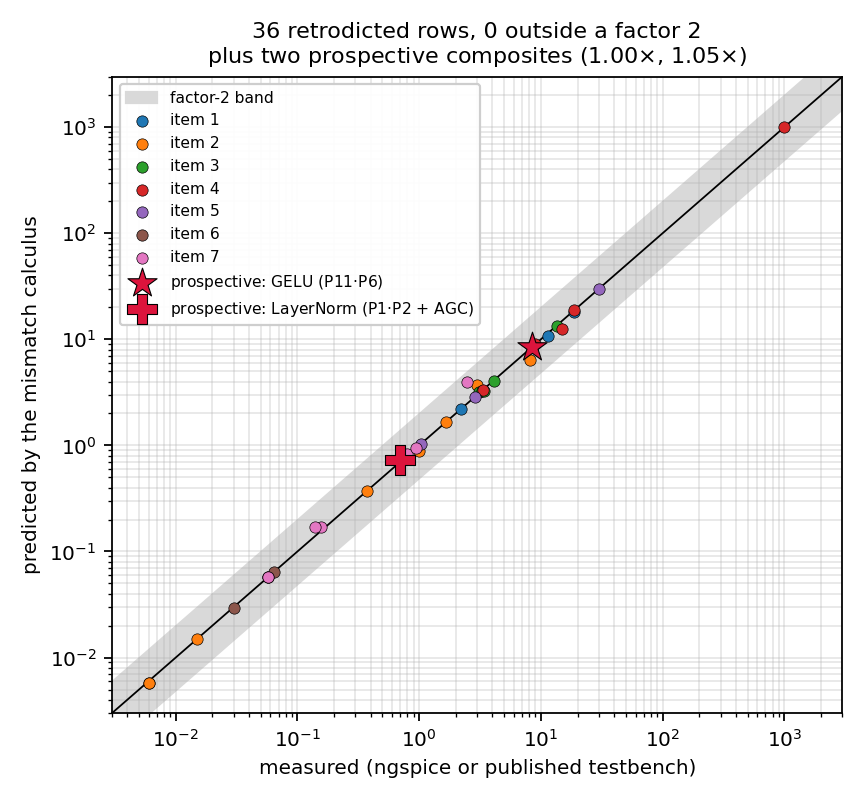
\includegraphics[width=0.52\textwidth]{fig_v3_calculus.png}
\caption{Pre-registered test of the mismatch calculus. Grey band: factor 2. Circles: the 36 retrodicted rows, grouped by item; none falls outside the band, worst $1.63\times$. Red markers: the two prospective composites, predicted before the arbitrating circuit simulations were run ($1.00\times$ and $1.05\times$ on the per-channel median). Figure regenerated from the stored numerical results; see \texttt{spice/make\_v3\_figures.py}.}
\label{fig:calculus}
\end{figure}

\paragraph{Two design findings obtained without building a circuit.} First, \textbf{GELU is unprotected}: $8.5\%$ per-channel error at the MOS-typical corner, $12\times$ the AGC-normalized VGA residual, and half of it from a sigmoid pair whose offset is amplified exactly on the channels carrying least signal (R12), so no downstream normalization removes it. \S\ref{sec:training} tests whether training can, and finds that it removes only the gain-like two thirds. Second, \textbf{LayerNorm's mean mirror costs $0.31\%$ per channel} because its \textit{shared} error is orthogonal to the centred signal (R3$'$)---a shared device behaving as a per-channel error source, confirmed by ablation on the same input draw.

\paragraph{Limitations.} The calculus inherits every limitation of the simulations it reproduces and cannot be more right than they are: junction-exact but wiring-ideal, one technology model, no PDK. The levers $L\approx19$--$23$ are properties of \textit{these} biases; on a real process the rules survive and the constants do not. Mismatch is assumed independent, and the correlated case is known to be \textit{worse}, so this is optimistic. Three of the seven retrodiction items are algebraic identities or re-derivations rather than approximations, so the evidence that a \textit{lossy} tuple suffices rests on four items plus the prospective test, and R12 has exactly one use. Finally the metric removes a scalar, which is right for a normalization layer and wrong for a stage whose absolute gain matters: the GELU common mode of $9$--$10\%$ is real and is not obviously benign.

\subsection{Phase 3: Multi-Computation Fusion}

After domain assignment, the compiler searches for subgraph patterns matching known multi-computation classes (Table~\ref{tab:fusion})~\cite{bieg2026}:

\begin{table}[h]
\centering
\caption{Multi-computation fusion patterns.}
\label{tab:fusion}
\small
\begin{tabular}{lll}
\toprule
Pattern & Class & Multiplier \\
\midrule
\{P3, P5\} adjacent & Race & $5\times$ \\
\{P1, P2\}$^{2+}$ Laplacian & Equilibrium & $4$--$12\times$ \\
\{P3, P5, P4, P1\} & Race-Loss & $6\times$ \\
\{P10, P7, P1, P2\} & Threshold/Ising & $2$--$3\times$ \\
\{P11, P1, P2, P8\} AGC & Normalization & $4\times$ \\
\bottomrule
\end{tabular}
\end{table}

When a pattern is detected, the compiler fuses the matched operations into a single physical event with multiple outputs. For example, Softmax followed by Cross-Entropy Loss contains the pattern \{P3, P5, P4, P1\}, which maps to a single sMTJ race event yielding both the softmax sample and $-\log p_{\text{correct}}$ simultaneously~\cite{bieg2026}.

\subsection{Phase 4: Transition Minimization}
\label{sec:transitions}

\begin{definition}[Transition Minimization Problem]
Given graph $G$ with nodes assigned to \textsc{physics} or \textsc{digital}, find the minimum number of domain transitions (ADC/DAC conversions) in any valid topological execution order.
\end{definition}

Each transition incurs cost:
\begin{itemize}[leftmargin=*]
\item ADC (analog $\to$ digital): ${\sim}100$~fJ, ${\sim}1$~ns latency
\item DAC (digital $\to$ analog): ${\sim}50$~fJ, ${\sim}0.5$~ns latency
\item Quantization noise added per transition
\end{itemize}

\textbf{Heuristic}: Identify ``physics islands'' (connected analog subgraphs), then greedily merge adjacent islands when merging reduces total transitions. For a standard transformer layer, the optimal partition requires 4 transitions (2 ADC + 2 DAC)---two physics islands per layer (the attention and FFN nonlinearities), each bracketed by one ADC/DAC pair; the diagram below shows one such island:

\begin{equation*}
\underbrace{[\text{QKV MatMul}]}_{\text{digital}} \!\xrightarrow{\text{ADC}}\! \underbrace{[\text{Softmax+RMSNorm+GELU}]}_{\text{physics}} \!\xrightarrow{\text{DAC}}\! \underbrace{[\text{FFN MatMul}]}_{\text{digital}}
\end{equation*}

\noindent\textit{Note}: This diagram shows the partitioning for a digital-weight architecture (e.g., GPU or SRAM-CIM). On crossbar-based chips (e.g., IBM PCM, memristive arrays), MatMul maps to physics via P1$\cdot$P2, yielding a fully analog pipeline with only peripheral ADC/DAC.

Two additions to the transition accounting follow from \S\ref{sec:domain} and \S\ref{sec:calculus}. First, the \textbf{same-node rule} (R7): a transition is not something the compiler pays for at the domain boundary only, it is something a \textit{placement} decision can remove entirely. If the P8 accumulator node and the P5 race driver are the same physical node, a selection costs no conversion at all; if they are not, every MCTS simulation re-drives $b\cdot d = 256$ DAC channels at 12.8~pJ and 256 settling times (\S\ref{sec:recursion}). Second, \textbf{rewrite latency is a transition cost}: a memristive write of 10~ns--1~$\mu$s sits in the same budget line as an ADC, and above $t_{\mathrm{wr}} \approx 12$--$78$~ns it \textit{is} the budget (R8). \textit{Limitation}: both are structural preconditions rather than costs the heuristic can optimize away; the compiler can check them but cannot repair a placement it is not allowed to change.

\section{Resolving RMSNorm: The Last Open Mapping}
\label{sec:rmsnorm}

RMSNorm~\cite{zhang_rmsnorm2019}, used by LLaMA, Mistral, Gemma, Qwen, and DeepSeek, computes:
\begin{equation}
\text{RMSNorm}(\mathbf{x}) = \frac{\mathbf{x}}{\text{RMS}(\mathbf{x})} \cdot \gamma, \quad \text{RMS}(\mathbf{x}) = \sqrt{\frac{1}{N}\sum_{i=1}^{N} x_i^2}
\end{equation}

Normalization has been realized in analog before---a full-circuit memristor transformer carries a Layer Normalization module among its analog function blocks~\cite{yang2022}---but we have found no analog RMSNorm, and no prior treatment of normalization as a quantity \textit{pinned by a feedback constraint} rather than computed open-loop (\S\ref{sec:related}). We identify two implementations. Version~1 of this paper presented them as equally viable alternatives; circuit-level validation (\S\ref{sec:validation}) has since shown that they are not: the feedback implementation is robust to device mismatch, the open-loop pipeline is not. We therefore present the AGC feedback implementation as the primary mapping.

\subsection{Primary Implementation: AGC Feedback (Equilibrium)}
\label{sec:agc}

Automatic Gain Control circuits---standard in radio engineering since the 1920s---compute exactly RMSNorm:

\begin{enumerate}[leftmargin=*]
\item Input $x_i$ enters a Variable Gain Amplifier (VGA, Gilbert cell). \hfill [P11]
\item Output $y_i = G \cdot x_i$ is measured by an RMS detector. \hfill [P11$\cdot$P1$\cdot$P2]
\item Error signal ($\text{RMS}(y) - \gamma$) is integrated. \hfill [P8]
\item Integrator output controls VGA gain $G$. \hfill [feedback]
\item At equilibrium: $G = \gamma / \text{RMS}(x)$, so $y_i = \gamma \cdot x_i / \text{RMS}(x)$. \hfill [$\equiv$ RMSNorm]
\end{enumerate}

The key insight: \textbf{P12 (division by $\sqrt{\sigma^2}$) is computed implicitly by the feedback loop settling to equilibrium.} No explicit translinear divider is needed. This is a Class~2.2 (Equilibrium) multi-computation~\cite{bieg2026}, yielding 4 observables:
\begin{enumerate}
\item Normalized output $y_i$ (primary)
\item Settled gain $G = 1/\text{RMS}(x)$ (quantization calibration)
\item RMS value (activation statistics)
\item Settling time (layer difficulty proxy)
\end{enumerate}

A second structural property, established by the validation in \S\ref{sec:validation}, turns out to be equally important: \textbf{mismatch tolerance}. Device mismatch in the RMS detector or integrator perturbs only the scalar loop target---equivalent to a slightly different $\gamma$, applied \textit{identically to all $N$ channels}. A common-mode scale factor on a normalization layer is functionally benign for a neural network. The only per-channel error source is the VGA array itself (one multiplier per channel), the minimal possible exposure.

\begin{remark}
This connection---RMSNorm = AGC---bridges three fields that have not previously been linked: (1)~radio engineering (AGC, 1925--present), (2)~computational neuroscience (divisive normalization, Carandini \& Heeger~\cite{carandini2012}), and (3)~ML hardware (normalization in CIM). The biological retina implements divisive normalization via shunting inhibition: a conductance-based mechanism mathematically equivalent to the translinear principle.
\end{remark}

\subsection{Alternative: Direct Translinear Pipeline (Open-Loop)}
\label{sec:translinear}

In current mode with $N$ parallel paths:

\begin{enumerate}[leftmargin=*]
\item \textbf{Square} ($\times N$): Gilbert cell in self-multiply mode: $I_i^2$. \hfill [P11]
\item \textbf{Sum}: KCL at common node: $I_{\Sigma} = \sum I_i^2$. \hfill [P1]
\item \textbf{Scale}: Current mirror with $1{:}N$ ratio: $I_{\text{ms}} = I_{\Sigma}/N$. \hfill [P2]
\item \textbf{Inv.\ sqrt}: 6-transistor translinear loop: $I_{\text{inv}} \propto 1/\sqrt{I_{\text{ms}}}$. \hfill [P12]
\item \textbf{Normalize} ($\times N$): Gilbert cell: $I_{\text{out},i} = I_i \cdot I_{\text{inv}}$. \hfill [P11]
\item \textbf{Scale}: Fixed mirror ratio $\gamma$. \hfill [P2]
\end{enumerate}

Propagation delay: ${\sim}12$~ns---a design estimate dominated by translinear settling, carried over from earlier versions and \textit{not} measured on any testbench in this paper. No clock, no ADC between steps.

\textbf{Factorization}: P11 $\cdot$ P1 $\cdot$ P2 $\cdot$ P12 $\cdot$ P11 $\cdot$ P2 = P1 $\cdot$ P2 $\cdot$ P11 $\cdot$ P12.

This pipeline is mathematically exact---validated to $<\!10^{-6}$ relative error with ideal junctions (\S\ref{sec:validation})---but every channel passes through two per-channel junction stages (squarer, output multiplier) \textit{open-loop}: device mismatch in these stages lands directly on the output as per-channel distortion. Under realistic mismatch it delivers only 1.5--4.5 effective bits (Table~\ref{tab:mismatch}) and should be used only with per-device trimming or calibration.

\subsection{Circuit-Level Validation}
\label{sec:validation}

We validate both implementations in ngspice-46 at a deliberately defined fidelity: \textbf{junction-exact, wiring-ideal}. All log-domain arithmetic is performed by real diode $I$--$V$ characteristics (the exponential junction law, i.e.\ the actual physics of P3/P4/P12); the translinear loop wiring is replaced by ideal voltage summation. This isolates the question ``what does device physics do to the computation?'' from bias-network engineering. The testbenches (over 17{,}000 simulation runs, $N=8$--$128$ channels, code in the repository under \texttt{spice/}) cover:

\begin{enumerate}[leftmargin=*]
\item \textbf{Ideal-device DC operating-point analysis} of the translinear pipeline (\S\ref{sec:translinear}).
\item \textbf{Monte-Carlo mismatch} (200 runs per corner): lognormal spread on saturation current $I_s$, normal spread on ideality factor $n$, and gain error on the $1{:}N$ mirror, at three technology corners (Table~\ref{tab:mismatch}).
\item \textbf{Continuous-time transient} of the AGC loop (\S\ref{sec:agc}) with a real integration capacitor (1~pF, $\mu$A-scale currents, RMS-detector time constant 0.5~ns), including a $2.5\times$ input step.
\item \textbf{AGC-path mismatch decomposition}: the RMS detector built from real mismatched junctions, loop equilibrium found by bisection on the SPICE-measured detector output, and the output error split into common-mode gain shift vs.\ per-channel residual---separately for detector-side and VGA-side mismatch, and swept over $N=8/32/128$.
\item \textbf{Paired softmax comparison}: sum-feedback AGC normalization vs.\ open-loop translinear softmax, both sharing identical mismatched exponential stages.
\end{enumerate}

\textbf{Result 1: the mathematics is confirmed at circuit level.} With ideal devices, the junction law reproduces RMSNorm to a mean relative error of $1.1\times10^{-7}$ (max $2.8\times10^{-7}$). The physics genuinely computes the right function.

\textbf{Result 2: the open-loop pipeline is mismatch-fragile.} The dominant mechanism is ideality-factor mismatch: a log-domain junction voltage is $n V_T \ln(I/I_s)$ with $\ln(I/I_s) \approx 23$ at $\mu$A currents, so a $0.3\%$ spread in $n$ between devices becomes a ${\sim}7\%$ current error---the classic matching problem~\cite{pelgrom1989} amplified by the full log magnitude. Table~\ref{tab:mismatch} gives the Monte-Carlo results (error measured against the unit-RMS reference output):

\begin{table}[h]
\centering
\caption{Open-loop translinear RMSNorm under Monte-Carlo mismatch (200 runs per corner, $N=8$, ngspice). Error is absolute against the unit-RMS reference output.}
\label{tab:mismatch}
\small
\begin{tabular}{lccccc}
\toprule
Corner & $\sigma_{I_s}$ & $\sigma_n$ & $\sigma_{\text{mirror}}$ & mean / p95 error & eff.\ bits \\
\midrule
BJT-grade & 1\% & 0.05\% & 0.5\% & 2.2\% / 4.5\% & ${\sim}4.5$ \\
Subthreshold MOS, typical & 3\% & 0.3\% & 1\% & 11.4\% / 22.9\% & ${\sim}2.1$ \\
Subthreshold MOS, worst & 5\% & 0.5\% & 2\% & 18.7\% / 34.4\% & ${\sim}1.5$ \\
\bottomrule
\end{tabular}
\end{table}

\textbf{Result 3: the AGC loop settles fast, and closes to $<10^{-3}$ under a realistic integrator.} From a cold start the loop reaches the 1\% band of the exact gain $G = \gamma/\text{RMS}(x)$ in \textbf{4.4~ns}; after a $2.5\times$ input step it re-settles in \textbf{5.3~ns} (Figure~\ref{fig:spice}), and the per-channel outputs match exact RMSNorm to $\leq\!3\times10^{-6}$. \textit{Corrected in v3}: the equilibrium gain error quoted in v2 as ``below $10^{-4}$'' is an ideal-integrator number. With an infinite-DC-gain integrator the loop closure is $3\times10^{-10}$; with a realistic \textbf{60~dB integrator DC gain} it is $7.2\times10^{-4}$, i.e.\ \textbf{below $10^{-3}$ but seven times above the figure v2 stated} (\S\ref{sec:gaps}). Settling is robust: none of four non-idealities moves it by more than 40~ps, and the worst case across all of them is 5.30~ns. The feedback implementation is thus faster at these bias conditions than the open-loop pipeline, but only against the latter's ${\sim}12$~ns \textit{estimate} (\S\ref{sec:translinear}), which is a design figure rather than a simulated one, so this particular comparison is the weakest in this section; settling scales with the detector time constant and loop bandwidth, both design choices---and \S\ref{sec:gaps} shows that this particular choice is 2.9$\times$ away from the optimum of its own topology.

\begin{figure}[t]
\centering
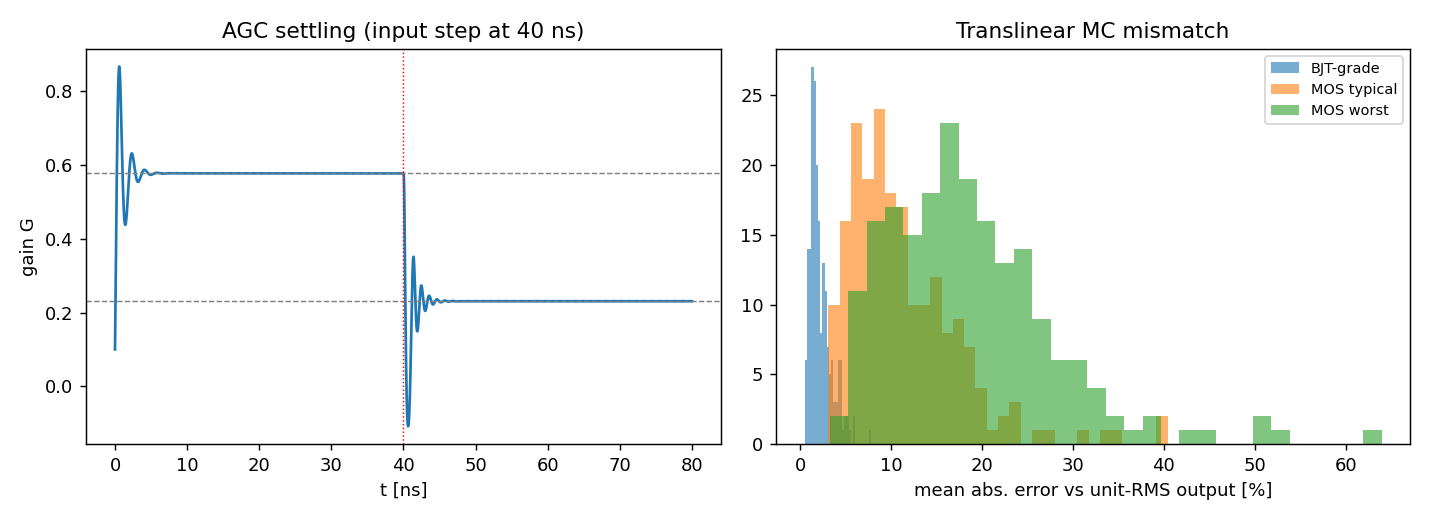
\includegraphics[width=\textwidth]{fig_rmsnorm_spice.png}
\caption{Circuit-level validation. \textbf{Left}: AGC gain transient (ngspice, real 1~pF integration capacitor). The loop settles to the exact RMSNorm gain in 4.4~ns from cold start and re-settles in 5.3~ns after a $2.5\times$ input step at $t=40$~ns (dashed lines: exact targets). \textbf{Right}: Monte-Carlo mismatch distributions for the open-loop translinear pipeline at three technology corners; in the feedback implementation, the corresponding detector-side mismatch shifts only the common-mode gain and produces no per-channel distortion by construction (quantified in Table~\ref{tab:agcsweep}).}
\label{fig:spice}
\end{figure}

\textbf{Result 4: the common-mode argument, simulated.} With the RMS detector built from real mismatched junctions and the loop closed around it, the error decomposition (Table~\ref{tab:agcsweep}) is unambiguous: detector-side mismatch produces \textit{exactly zero} per-channel distortion at every corner. The zero itself is architectural rather than statistical---the signal path traverses only the VGA, so detector errors \textit{can} only move the scalar gain; what the junction-level simulation adds is the \textit{magnitude} of that gain shift under realistic mismatch (1--8\% median, i.e.\ a slightly different $\gamma$, trimmable with a single per-layer measurement). The sole per-channel exposure is the VGA array, whose residual tracks $\sigma_{\text{VGA}}$ ($0.7$--$0.8\,\sigma_{\text{VGA}}$ at $N=8$; $0.7$--$0.95\,\sigma_{\text{VGA}}$ once $N$ is swept, \S\ref{sec:training}) with negligible common-mode contribution; the two contributions add without cross terms. Sweeping $N=8\to128$, the detector-induced gain shift shrinks toward a floor set by the \textit{scalar} devices (mirror, reference)---which are themselves common-mode and hence equally trimmable---while the VGA residual stays flat, as the per-channel/shared-path structure predicts. \textit{Both italicized statements are revised in \S\ref{sec:gaps}}: the floor is a Jensen bias of the \textit{per-channel} devices rather than a scalar-device floor (Test~2), and noise adds a second per-channel exposure on the VGA (Test~4).

\begin{table}[h]
\centering
\caption{AGC-path mismatch decomposition (junction detector, loop closed by bisection, 100 MC runs per cell, $N=8$). Error split into common-mode gain shift vs.\ per-channel residual; median / p95.}
\label{tab:agcsweep}
\small
\begin{tabular}{lcc}
\toprule
Mismatch location & Common-mode & Per-channel \\
\midrule
Detector only, BJT-grade & 1.0\% / 2.7\% & \textbf{0.000\%} / 0.000\% \\
Detector only, MOS typical & 3.0\% / 10.3\% & \textbf{0.000\%} / 0.000\% \\
Detector only, MOS worst & 8.1\% / 20.2\% & \textbf{0.000\%} / 0.000\% \\
VGA only, $\sigma=0.5\%$ & \textbf{0.0007\%} / --- & 0.37\% / 0.67\% \\
VGA only, $\sigma=1\%$ & \textbf{0.0024\%} / --- & 0.69\% / 1.16\% \\
VGA only, $\sigma=2\%$ & 0.015\% / 0.031\% & 1.66\% / 2.45\% \\
Both (MOS typ.\ + VGA 1\%) & 4.3\% / 11.5\% & 0.75\% / 1.28\% \\
\bottomrule
\end{tabular}
\end{table}

\textit{Corrected in v3}: the ``$0.006\%$'' entries reported in v2 for the VGA-only common mode are not physics---they are the quantization floor of the 16-step bisection used to close the loop, whose own resolution is $1.0\times10^{-4}$ relative $=0.010\%$ (rule R15). With a converged solver the true values are $\mathbf{0.0024\%}$ at $\sigma_{\mathrm{VGA}}=1\%$ and $\mathbf{0.0007\%}$ at $0.5\%$, i.e.\ genuinely second order in $\varepsilon$ as theory requires, the first-order terms cancelling between the gain solution and the fit. The direction matters: the qualitative claim---that the VGA residual tracks $\sigma_{\mathrm{VGA}}$ with \textit{negligible} common-mode contribution---becomes stronger by a factor 2.5--9, not weaker. The three detector rows are unaffected; their common mode is percent-scale, far above the floor.

\textbf{Result 5: the pattern generalizes---softmax.} Replacing the RMS detector by a sum detector pins $\sum_i y_i = 1$ at equilibrium, turning the same loop into softmax ($y_i = e^{x_i}/\sum_j e^{x_j}$; the settled gain is $1/Z$, so the partition function comes for free). Analog softmax circuits are classical---Elfadel and Wyatt derived softmax as a multiterminal analog circuit element in 1993~\cite{elfadel1993}, open-loop translinear realizations exist~\cite{sillman2023}, and a concurrent time-domain realization with an RC-tunable temperature has been reported in 22~nm FDSOI~\cite{singh2026}, which is the domain choice \S\ref{sec:domain} compares against the log domain; what is compared here is their mismatch behavior against the feedback realization. In a paired Monte-Carlo comparison where both variants share identical mismatched exponential stages, the sum-feedback AGC beats the open-loop translinear softmax by $3.1$--$3.4\times$ in median $L_1$ error at all three corners (MOS typical: 13.6\% vs.\ 4.1\%); it settles in 3.2~ns from cold start and 2.1~ns after a logit switch, with equilibrium error $<\!10^{-7}$. The improvement is smaller than for RMSNorm for an instructive reason: the exponential stage (P3) sits \textit{before} the loop and keeps its per-channel exposure---feedback protects the normalization path, not the primes upstream of it.

\textbf{Why feedback wins---the structural argument.} In the open-loop pipeline, each channel's signal traverses per-channel junction stages whose individual errors appear directly in that channel's output: mismatch becomes \textit{per-channel distortion}, i.e.\ noise on the activations. In the AGC loop, the RMS detector and integrator act on a \textit{single scalar}; any mismatch there shifts the settled gain identically for all channels---equivalent to a slightly different $\gamma$, which a trained network absorbs. Result~4 confirms this mechanism directly. Feedback thus converts the dominant analog failure mode from per-channel noise into a benign common-mode scale, and does so exactly for everything downstream of the loop input (Result~5 delimits the protection: upstream primes stay exposed). This inverts the presentation of v1: the translinear pipeline is the fallback (usable with trimming), the AGC loop is the mapping.

\textbf{What this validation did not cover, and what \S\ref{sec:gaps} now does.} Version~2 listed four gaps: idealized loop wiring (no bias-network errors, no Early effect); thermal noise and temperature gradients not modeled; DC testbenches driving magnitude currents whereas RMSNorm inputs are signed, so that the per-channel output stage and the VGA require four-quadrant (Gilbert/class-AB differential) signaling; and $N$ swept only to 128 rather than 4096. Each is closed below as a \textit{pre-registered test against this paper's own claims}, not as a confirmation exercise. Four of the claims under test needed correcting as a result: two (Result~3's loop closure, Table~\ref{tab:agcsweep}'s VGA common mode) are corrected in place above, and two (Result~4's mechanism sentence, the per-channel exposure ranking) are corrected in the tests themselves.

\subsection{Closing the Four Validation Gaps}
\label{sec:gaps}

Eight claims were placed under test, each with a numerical criterion fixed in writing before any new code was run, together with an explicit statement of what would make the author wrong. The pre-existing testbench was first replayed to reproduce the published Table~\ref{tab:agcsweep} rows within 15\%---achieved to $0.3\%$ and $0.6\%$ on the two gated rows---before a line of new code existed. Five pre-registered predictions turned out to be wrong and are flagged as such below.

\subsubsection{Test 1 --- four-quadrant signalling}

The magnitude-current VGA is replaced by a differential four-quadrant multiplier. Signed $x_i$ is split into two strictly positive rails, either class-AB ($x^\pm = (\sqrt{x^2+4I_b^2}\pm x)/2$, so that $x^+ - x^- = x$ and $x^+x^- = I_b^2$) or class-A ($x^\pm = I_b \pm x/2$ with $I_b$ large enough to keep both rails positive). Each rail passes its own translinear multiplier with an independent output mirror error; the detector keeps the junction RMS chain, fed by a \textit{mismatched full-wave rectifier} with its own per-branch gain error and a swept dead-zone. Criterion: \textit{if with signed signals the detector-side per-channel residual is no longer zero ($>0.05\%$) or the VGA-side residual exceeds $1.2\,\sigma_{\mathrm{VGA}}$, the four-quadrant extension breaks the common-mode story.}

\textbf{Result: pass, conditional on class-AB.} Detector-side per-channel residual stays at the architectural zero---$\le 10^{-5}\%$, i.e.\ numerical zero---with signed inputs, a mismatched rectifier \textit{and} a rectifier dead-zone, for the reason the structural argument gives: the signal path traverses only the VGA, so everything in the detector, rectifier included, can only move the scalar gain. The VGA-side residual is $\mathbf{0.679\,\sigma_{\mathrm{VGA}}}$ for class-AB against a magnitude-only baseline of $0.672$---four-quadrant signalling costs \textit{nothing}. \textbf{Class-A fails at $1.79\,\sigma_{\mathrm{VGA}}$} and must be excluded explicitly. The governing quantity is not ``four-quadrant'' but the standing current: the per-channel variance is $\mathrm{Var}(e_i) = G^2\sigma^2_{\mathrm{VGA}}(x_i^{+2} + x_i^{-2})$, and class-AB reaches the $x^{+2}+x^{-2} = x^2$ limit exactly because only one rail conducts at a time, while class-A never does. An analytic column tracks the measurement across a $5\times$ range of residual, and the residual/$\sigma$ ratio is flat in $\sigma_{\mathrm{VGA}}$ ($0.681/0.679/0.676$ at $0.5/1/2\%$), so this is a linear scaling law and not a fitted constant. The pre-registered prediction of $0.8$--$0.9\,\sigma$ for class-AB was \textbf{wrong}---it double-counted a decomposition that does not apply when only one rail conducts---and the correct statement is stronger.

Two by-products. The additivity claim of Result~4 is confirmed to four digits: the quadrature of the detector-only and VGA-only cells is $0.6791\%$ and the combined measurement is $0.6791\%$. And a class-AB \textbf{rectifier dead-zone} is a new named common-mode term: $0.2\,\mu$A of dead-zone produces a deterministic $15.03\%$ gain error with \textit{zero} variance and zero per-channel distortion---large, but a pure $\gamma$ shift and therefore trimmable. \textit{Limitation}: the rectifier is behavioural. Its mismatch and dead-zone are captured; its speed, charge injection and behaviour on fast zero crossings are not, and none of them is visible to a DC testbench.

\subsubsection{Test 2 --- detector dynamic range at $N = 4096$}

Three current-scaling schemes were declared before running: (a)~per-channel current fixed at $1\,\mu$A so that the summing node grows to 4.1~mA at $N=4096$; (b)~sum-constant, shrinking the per-channel current to keep the summing node at ${\sim}8\,\mu$A; (c)~a stress variant placing a diode-connected device \textit{at} the summing node with a realistic series resistance. Criterion: \textit{if the ideal-device error at $N = 4096$ exceeds $10^{-3}$ or the per-channel residual grows with $N$, the extrapolation claimed in v2 fails.}

\textbf{Result: pass for the published topology, and the extrapolation is now conditional on two design choices v2 never stated.} Scheme~(a) is flat in $N$ at ${\sim}10^{-7}$: $1.54\times10^{-7}$ at $N=8$ and $\mathbf{1.09\times10^{-7}}$ at $N=4096$, four orders below the criterion. Scheme~(b) reaches $7.4\times10^{-5}$---worse by a factor 700, driven by the simulator's conductance floor, but \textit{not} a failure; the pre-registered prediction that it would cross $10^{-3}$ was wrong in magnitude though right in direction, and the crossing sits below ${\sim}0.5$~nA per channel. Scheme~(c) fails emphatically at \textit{every} $N$ ($1.3\times10^{-2}$ already at $N=8$, $2.7\times10^{3}$ at $N=4096$): 4.1~mA through 50~$\Omega$ is a 0.2~V ohmic drop on a junction whose entire signal swing is ${\sim}0.6$~V. \textbf{So the summing node must stay at virtual ground, and the per-channel current must not be scaled down to keep the summing current constant.} With those two conditions, ``structural rather than speculative'' is earned.

The per-channel residual does \textbf{not} grow with $N$: it rises from $0.79\%$ at $N=8$ to $1.00\%$ at $N=4096$ and saturates, and the entire $N$-dependence is R3's projection factor $\sqrt{1-\sum_i w_i^2}$, whose measured-to-predicted ratio goes to $1.000$ at $N=4096$. ``Flat in $N$'' therefore means \textit{asymptotically} $\sigma_{\mathrm{VGA}}$, not constant from $N=8$.

\textit{Correction to Result~4's mechanism sentence.} Version~2 said the detector-induced shift shrinks toward ``a floor set by the scalar devices (mirror, reference)''. The shrink is real ($2.645\% \to 0.739\%$ for the per-channel devices between $N=8$ and $N=4096$) but it does not go to zero, and the residue is not a scalar device: it is a deterministic Jensen bias of the per-channel devices themselves. With $\mathrm{Var}(v) = 5\sigma_{I_s}^2 + 5(L\sigma_n)^2$ and $L = \ln(I_{\mathrm{unit}}/I_s) = 23.03$, $\mathbb{E}[\mathrm{ms}]/\mathrm{ms}_{\mathrm{true}} = e^{\mathrm{Var}/2} = 1.0143$, a $+1.43\%$ bias on the mean square $=\mathbf{+0.71\%}$ on the gain, independent of $N$; measured $0.739\%$, a $3.5\%$ agreement. Meanwhile the true scalar floor is $2.6$--$3.0\%$ and is dominated by the \textbf{reference diode}, not the mirror: a $0.3\%$ ideality spread on the single reference shifts its log voltage by 1.8~mV, and $e^{1.8\,\mathrm{mV}/V_T} = 1.072$, i.e.\ $7\%$ on the mean square. Both contributions remain common-mode and trimmable, so the conclusion survives; the mechanism sentence does not. \textit{Limitation}: $N = 4096$ is DC-only. No 4096-channel transient was run---settling is a property of the loop, not of $N$---but a 4096-channel \textit{layout} would add distribution parasitics on the gain rail that this model has no representation of.

\subsubsection{Test 3 --- loop wiring one notch less ideal}

Four non-idealities, each parameterized and each testable alone: Early effect on the mirrors ($V_A \in \{20, 50\}$~V), a $1\%$ bias-network error on the reference currents, a finite integrator DC gain of 60~dB realized as a leak resistor across the integrating capacitor, and $2\%$ integrator-capacitor mismatch. Two different ``equilibrium gain errors'' are reported separately, because v2's $10^{-4}$ and its $1$--$8\%$ are not the same quantity: \textit{loop closure} $|\langle y^2\rangle - \gamma^2|/\gamma^2$ at settlement, and the \textit{absolute} error against exact RMSNorm, which absorbs every detector and reference offset. Criterion: \textit{if the equilibrium gain error exceeds $10^{-2}$ or settling exceeds 20~ns, the ``4--6~ns, $<10^{-4}$'' claim depends on the idealization.}

\textbf{Result: pass on both criteria---but the ``$<10^{-4}$'' headline does not survive.} Worst loop closure $7.2\times10^{-4}$ against a $10^{-2}$ bar. Only the finite integrator gain touches it, moving it from $3\times10^{-10}$ to $7.2\times10^{-4}$. Worst settling 5.30~ns against a 20~ns bar, with no non-ideality moving settling by more than 40~ps. Worst absolute gain error $1.32\%$, which lands inside the $1$--$8\%$ common-mode band Result~4 already declares trimmable; Early effect and bias-network error move \textit{only} this quantity and leave loop closure untouched.

The one genuinely new term is the \textbf{per-channel Early residual}: the VGA output mirror sits in the signal path, so its $V_{CE}$-dependent gain error is signal-correlated and is \textit{not} demoted by the loop---the single mechanism in this test that feedback does not cover. It is $0.0623\%$ at $V_A = 20$~V and $0.0249\%$ at 50~V, i.e.\ ${\sim}11\times$ below the $0.69\%$ VGA-mismatch residual. It is a distortion rather than a noise. The pre-registered prediction of $0.30\%$ was pessimistic by ${\sim}5\times$. \textit{Limitation}: the translinear loop wiring is still voltage summation by controlled sources. A real stacked translinear loop adds base-current errors, $V_{CE}$-dependent saturation currents and emitter-degeneration effects that this fidelity level cannot see.

\subsubsection{Test 4 --- thermal and shot noise, and the third per-channel exposure}
\label{sec:noise}

Every junction carrying DC current $I$ was given white current noise of one-sided PSD $2qI$ and every resistor $4kT/R$, injected as explicit time-domain sources whose in-band PSD was probe-validated to $0.986$ of target; $I_0$, the current that unit amplitude represents, was swept over $\{0.1, 1, 10\}\,\mu$A, since the whole comparison is a bias-current question. Criterion: \textit{if the noise-induced per-channel error at the loop bandwidth exceeds the VGA-mismatch residual, noise rather than mismatch is the binding per-channel term and the exposure ranking changes.}

\textbf{Result: the criterion fires, and the formula that replaces the ranking is}
\begin{equation}
\boxed{\;\sigma_{\mathrm{pc}} \;=\; C\,\sqrt{k_j \cdot 2q\,B / I_0}\;}
\label{eq:noise}
\end{equation}
with $k_j$ the number of shot-noise junctions in the \textit{per-channel} signal path (2 for the current-log gain cell the VGA actually is) and $B$ the \textbf{declared observation bandwidth of the per-channel path}. The prefactor, fitted over six $(k_j, B)$ cells, is $C = \mathbf{0.780}$ (spread $0.770$--$0.800$ over the six cells) against a closed form for this input draw of $0.7664$, a ratio of $1.018$; for a flat draw $C = \sqrt{1-1/N}$, which is R3's residual factor, and the $0.766$ here is the crest factor of a Gaussian draw, because shot noise is loudest on the weak channels (R18). Per-channel agreement with the circuit simulator is $1.0001$--$1.012$ on all eight channels of the translinear GELU bench over a $26\times$ range of output current (and $1.00$--$1.06$ on the AGC array), and on the shared detector path predicted and measured spectral densities agree to ratio $1.000$---and to $7.744$ if R3's energy weights are dropped, which is the sharpest available evidence that those weights are load-bearing.

\begin{figure}[t]
\centering
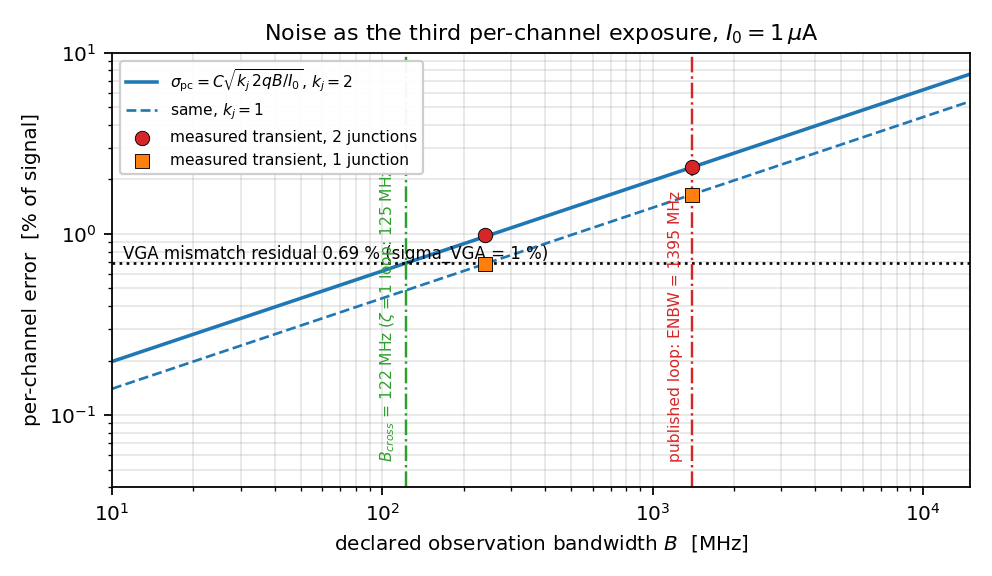
\includegraphics[width=0.72\textwidth]{fig_v3_noise.png}
\caption{Noise as the third per-channel exposure of the AGC array, at $I_0 = 1\,\mu$A. Lines: Eq.~\eqref{eq:noise} with $C = 0.780$ for a one- and a two-junction channel path. Markers: transient measurements on one bench under two bandwidth conventions. Dotted line: the $0.69\%$ VGA \textit{mismatch} residual of Table~\ref{tab:agcsweep}. Noise equals mismatch at $B = 122$~MHz, which coincides to 2\% with the noise bandwidth the published loop has when it is critically damped; at the loop's actual ENBW of 1395~MHz noise is $3.3\times$ mismatch.}
\label{fig:noise}
\end{figure}

\textbf{Where it crosses} (Figure~\ref{fig:noise})\textbf{.} At $I_0 = 1\,\mu$A the noise term equals the $0.69\%$ mismatch residual at $B_{\mathrm{cross}} = \mathbf{122}$~MHz for $k_j = 2$ (244~MHz for $k_j=1$). At the published loop's actual equivalent noise bandwidth of 1395~MHz, $\sigma_{\mathrm{pc}} = 2.0$--$2.3\%$, i.e.\ \textbf{$3.3\times$ the mismatch residual}, and equality would require $I_0 = 11.4\,\mu$A. Conversely, at $B = 100$~MHz equality falls at $I_0 = 0.82\,\mu$A. \textbf{The claim that ``the VGA array is the sole per-channel exposure'' is incomplete, not wrong}: the VGA array \textit{is} where everything lands---detector noise, like detector mismatch, produces a per-channel residual of $0.000000\%$ at every $I_0$ and in every detector configuration, the same architectural zero and for the same reason---but the VGA has \textbf{two} per-channel exposures, and the untrimmable one is the larger at the bandwidth that buys the advertised settling.

\textbf{Why $B$ is declared and not derived.} The strongest single result of this test is negative. Measured on the closed loop: the transfer from a channel's own VGA error to its own output is $0.909012$ at DC---exactly $1-w_0$---and $1.000003$ at high frequency, with an equivalent noise bandwidth of 121~GHz, while the transfer to a \textit{different} channel is $0.090988 = w_0$ at DC and $2.6\times10^{-6}$ at high frequency. \textbf{Above the loop bandwidth the loop does nothing at all to per-channel noise} (R19). So $B$ is not a loop property; it is the observation bandwidth of whatever consumes the output. The loop's own ENBW is a defensible default---a consumer slower than the loop would throw away the advertised settling spec---but it is a \textit{declared} quantity and must be stated as one.

\textbf{The damping rule.} The published loop ($k = 2\times10^{-3}$, $C_g = 1$~pF, $\tau_{\mathrm{det}} = 0.5$~ns) is \textbf{underdamped}, $\zeta = 0.299$, with $3.06\times$ gain-noise peaking at 473~MHz and a $+47\%$ first overshoot on a large-signal $2.5\times$ step ($+15.6\%$ small-signal); with no noise sources present at all the gain crosses its final value 40 times in 20~ns after a $2.5\times$ step. Underdamping does not \textit{add} noise---for this topology $\mathrm{ENBW} = \omega_n/(8\zeta) = \omega_c/4$ regardless of $\zeta$---but it decouples the settling envelope from the noise bandwidth by $\pi/(4\zeta^2) = 8.8\times$, which is exactly how a settling-derived band can be nine times too low. Because $\zeta\omega_n = 1/(2\tau_{\mathrm{det}})$ is \textit{independent of the loop gain}, lowering $k$ does not slow the envelope; it raises $\zeta$ and lowers the noise bandwidth. Critical damping is reached at
\[
k_{\mathrm{crit}} = \frac{C_g}{8\,G_0\,\mathrm{MS}(x)\,\tau_{\mathrm{det}}} = 1.79\times10^{-4},
\]
$11.2\times$ below the published value. There, \textbf{ENBW falls $11.2\times$ (1395 $\to$ 125~MHz) and $\sigma_{\mathrm{pc}}$ falls $3.34\times$ ($2.33\% \to 0.698\%$, i.e.\ onto the mismatch floor to within $1\%$) for a $1.34\times$ small-signal settling cost ($4.13 \to 5.52$~ns)}, and the peaking and the overshoot disappear entirely. That $B_{\mathrm{cross}} = 122$~MHz and the critically damped loop's own $\mathrm{ENBW} = 125$~MHz agree to $2\%$ is not a coincidence to exploit---it is the design point. A separate knob, a series resistor $R_z = \tau_{\mathrm{det}}/C_g = 500\,\Omega$ in the integrator, cancels the detector pole, removes the ringing and shortens settling $5.4\times$ to 0.77~ns, but at \textit{unchanged} bandwidth and therefore unchanged noise. The figure of merit $\sigma\sqrt{t_{\mathrm{settle}}}$ has a minimum at $\zeta = 1$: 4.74 at the published $\zeta = 0.30$, \textbf{1.64} at $\zeta=1$, $1.86$--$1.94$ when overdamped, ${\sim}2.02$ across the whole compensated first-order family. The published loop is $2.9\times$ off the optimum of its own topology.

\textit{Limitations.} $C$ is draw-dependent (0.766 here, 0.935 for a flat draw), so the crossover currents move with the input crest factor and are not universal constants; the cross-check was run at $N = 8$ on a single draw, deliberately, and the $N$-dependence of $C$ is asserted from the closed form rather than measured. Only white terms are modeled: flicker noise is absent and is not bandwidth-scalable, so Eq.~\eqref{eq:noise} is a \textit{lower} bound for any real cell. The $1.34\times$ settling cost at $k_{\mathrm{crit}}$ is a \textit{small-signal} cost---a large-signal step there is slew-limited and ${\sim}11\times$ slower---so a design that must track large steps keeps the higher loop gain and pays the noise, or adds a separate slew path. And $\sigma_{\mathrm{pc}} = 0.698\%$ at $k_{\mathrm{crit}}$ is Eq.~\eqref{eq:noise} evaluated at that loop's \textit{measured} bandwidth rather than a noisy transient; the formula is validated against noisy transients at 240 and 1395~MHz to $1.7\%$, so the extrapolation is short, but it is an extrapolation.

\subsubsection{Summary of the four tests}

Table~\ref{tab:gaps} collects the four verdicts, the decisive number behind each, and the claim of v2 that had to change as a result.

\begin{table}[h]
\centering
\caption{The four v2 validation gaps, closed as pre-registered tests. ``Correction'' lists the claims of v2 that had to change.}
\label{tab:gaps}
\footnotesize
\begin{tabular}{p{2.3cm}p{2.6cm}p{4.6cm}p{5.0cm}}
\toprule
Gap & Verdict & Decisive number & Correction to v2 \\
\midrule
Four-quadrant & \textbf{pass}, conditional on class-AB & detector-side per-channel $\le10^{-5}\%$; VGA residual $0.679\,\sigma_{\mathrm{VGA}}$ (class-A: $1.79$) & class-A must be excluded; dead-zone is a new common-mode term \\
$N = 4096$ & \textbf{pass} for the published topology & ideal-device error $1.09\times10^{-7}$; per-channel residual saturates at $1.00\,\sigma_{\mathrm{VGA}}$ & two design conditions stated; Result~4's ``scalar floor'' mechanism replaced by a $+0.71\%$ Jensen bias \\
Loop wiring & \textbf{pass} on both criteria & worst closure $7.2\times10^{-4}$; worst settling 5.30~ns & Result~3's ``$<10^{-4}$'' becomes ``$<10^{-3}$ at 60~dB loop gain''; per-channel Early residual $0.06\%$ is new \\
Noise & \textbf{criterion fires} & $\sigma_{\mathrm{pc}} = 0.78\sqrt{k_j 2qB/I_0}$; $3.3\times$ mismatch at the published bandwidth & noise is a third per-channel exposure; damping rule $k_{\mathrm{crit}}$ restores the ranking \\
\bottomrule
\end{tabular}
\end{table}

Temperature gradients, the fourth item in v2's list alongside thermal noise, are priced by rule R21 rather than simulated on this loop: a gradient is a \textit{gain}-type lever referred to the stage's reference device, and a 2~K gradient across eight channels costs an open-loop translinear GELU $1.41\%$ per channel---twice the whole VGA mismatch residual---but costs the AGC's current-log VGA $0.033\%$, a factor 43 less, because the translinear chain multiplies $\Delta T/T$ by $\ln(I/I_S)\approx19$ while a VGA multiplies it by $\ln G \approx 0.33$. \textit{Keep the temperature-sensitive quantity inside a ratio whose logarithm is small.} \textit{Limitation}: this holds at channel granularity; a gradient \textit{across} one differential pair's two devices becomes an offset-type lever at ${\sim}3.7$~mV/K, so the granularity of the thermal model decides the class---and a gradient across a 4096-channel array would be spatially correlated, which is exactly the case R3's independence assumption excludes.

\subsection{Full LayerNorm Extension}

For models requiring mean subtraction (GPT-2, GPT-3):
\begin{enumerate}[leftmargin=*]
\item $\mu = (1/N)\sum x_i$: current mirror sum + divider. \hfill [P1$\cdot$P2]
\item $\tilde{x}_i = x_i - \mu$: KCL subtraction (broadcast $\mu$ via mirrors). \hfill [P1]
\item Apply RMSNorm to $\tilde{x}_i$ (AGC feedback, \S\ref{sec:agc}). \hfill [P11$\cdot$P1$\cdot$P2$\cdot$P8]
\item Add bias $\beta$: current injection. \hfill [P1]
\end{enumerate}

Additional delay: ${\sim}2$~ns for current mirror settling, giving ${\sim}7$~ns in total. \textit{Both figures are design estimates carried over from earlier versions, not simulation results}---no testbench in this paper measures them, and they should not be read at the same confidence as the accuracy numbers that follow.

\textbf{What the upgrade costs, measured.} The mean path sits \textit{upstream} of the loop input, so feedback gives it no protection; and because the centred signal is orthogonal to the all-ones vector, \textit{both} the shared $1{:}N$ mirror error and the per-channel copy errors land in the per-channel residual (rule R3$'$). The mismatch calculus predicted $0.723\%$ per channel and a circuit simulation measured $0.690\%$; an ablation on the same input draw, with the mean-path mirrors set to ideal, gives $0.615\%$, so the implied mean-path contribution is $\mathbf{0.31\%}$ against a predicted $0.24$--$0.30\%$. The cost of upgrading RMSNorm to LayerNorm is therefore $\sqrt2\,|\mathrm{mean}(x)|\,\sigma_{\mathrm{mirror}}/\mathrm{RMS}(x-\mathrm{mean}(x))$ of extra per-channel error---here $0.31\%$ on top of $0.62\%$, making the layer ${\sim}12\%$ worse. It scales with the input's own mean-to-deviation ratio, so it is free for zero-mean activations and expensive for biased ones: a compile-time check the compiler can perform on activation statistics it already has. \textit{Limitation}: measured at one corner, $N=8$, one input draw, at the wiring-ideal fidelity level; the current mirrors carry a stated gain error rather than a modelled output impedance.

\section{Feedback as a Design Principle Extends to Training}
\label{sec:training}

The validation of \S\ref{sec:validation} is a statement about a forward pass: a quantity pinned by a loop constraint is protected from device mismatch in a way that the same quantity computed open-loop is not. The same principle read one level up makes a different and testable claim. A gradient \textit{measured on the mismatched physical circuit} contains that circuit's mismatch, so a trained parameter can absorb it; a gradient taken from an idealized digital model does not, and cannot. This section tests that claim, isolates the structural property the backward path must have, and identifies where the mechanism stops working.

The stage under test is the RMSNorm/AGC stage of \S\ref{sec:agc} with its trainable per-channel affine $\gamma$, followed by a frozen linear read-out $W \in \mathbb{R}^{M\times N}$, $M=4$; targets come from the ideal network, so the task is exactly ``undo the mismatch''. The metric is the same error decomposition used throughout: a least-squares scalar is removed per test sample and the residual RMS is reported, in units of $\sigma_{\mathrm{VGA}}$.

\subsection{Five gradient sources on identical mismatch draws}

Five conditions differing only in where the gradient comes from are compared on identical mismatch draws (Table~\ref{tab:trainconds}).

\begin{table}[h]
\centering
\caption{The five conditions. Within a mismatch draw, all conditions see the same device mismatch $\varepsilon$, the same training and test sets, the same $W$, the same backward matrix and the same optimizer schedule; only the gradient source differs. Plain SGD with a cosine-decayed rate is used in every condition, chosen after checking that it does not disadvantage condition~D (an adaptive optimizer does).}
\label{tab:trainconds}
\footnotesize
\begin{tabular}{p{1.1cm}p{3.6cm}p{6.2cm}p{4.0cm}}
\toprule
& forward & backward & lineage \\
\midrule
A & \textbf{ideal} model & exact gradient of the ideal model; the learned $\gamma$ is then \textit{deployed} on the mismatched forward and measured there & train-in-simulation \\
B & \textbf{mismatched} circuit & exact gradient of the \textbf{ideal} model & physics-aware training~\cite{wright2022} \\
C & mismatched circuit & \textbf{fully random} $B$ in place of $W^{\mathsf T}$, plus a per-channel backward gain mismatch & feedback alignment~\cite{lillicrap2016} \\
C2 & mismatched circuit & random magnitudes but the \textbf{signs of $W$}, same backward gain mismatch & sign symmetry~\cite{liao2016,xiao2018} \\
D & mismatched circuit & \textbf{none}; two-sided random perturbation of $\gamma$ & perturbative / extremum seeking~\cite{cauwenberghs1996,leblanc1922,krstic2000} \\
\bottomrule
\end{tabular}
\end{table}

Four criteria were fixed before running. \textit{Criterion~1}: if condition~A already reduces the per-channel residual below $0.35\,\sigma$, the residual was not a mismatch effect and the experiment is uninformative. \textit{Criterion~2}: if condition~B does not reduce it below $0.2\,\sigma$, the claim that a physically measured gradient absorbs the mismatch is killed. \textit{Criterion~3}: if condition~C ends above $2\times$ condition~B, the feedback-alignment relaxation is killed for this setting. \textit{Criterion~4}: if condition~D needs more than $200\times$ the forward evaluations of B, the perturbative route is impractical---a cost statement, not a kill.

\begin{figure}[t]
\centering
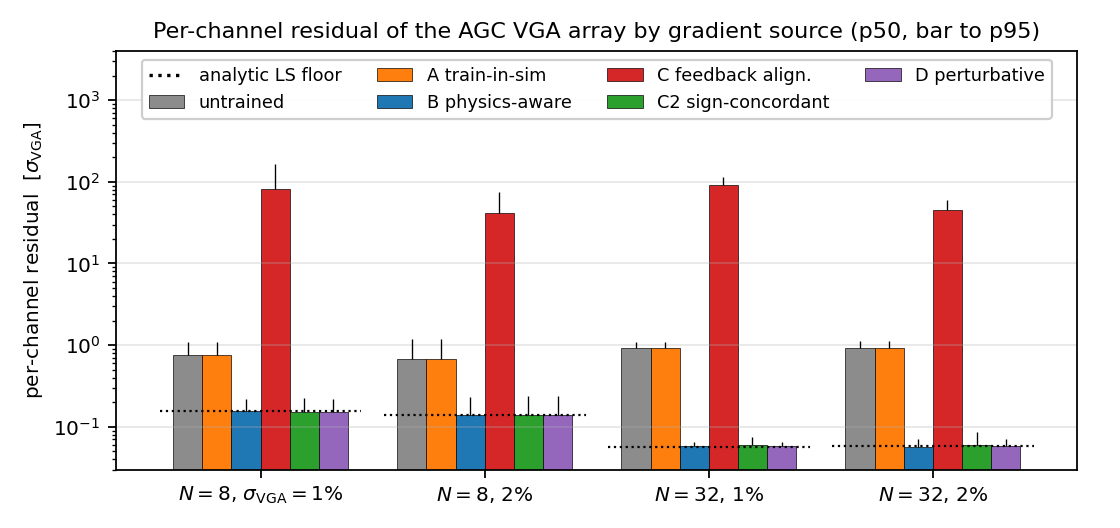
\includegraphics[width=0.92\textwidth]{fig_v3_training.png}
\caption{Per-channel residual of the AGC VGA array by gradient source, in units of $\sigma_{\mathrm{VGA}}$, over 20 Monte-Carlo mismatch draws per cell (bars: median; whiskers to p95; dotted line: the analytic least-squares floor of the training set). Train-in-simulation is bit-for-bit identical to untrained---$\gamma$ converges to 1. Physics-aware, sign-concordant and perturbative gradients all land \textit{on} the analytic floor. A fully random backward path diverges in every draw of every cell.}
\label{fig:training}
\end{figure}

\textbf{Results} (Figure~\ref{fig:training}; median over 20 draws per cell; cells are $N\in\{8,32\}\times\sigma_{\mathrm{VGA}}\in\{1\%,2\%\}$, in that order):

\begin{itemize}[leftmargin=*]
\item \textbf{Criterion~1 not triggered.} Condition~A gives $0.756 / 0.685 / 0.923 / 0.925\,\sigma$, identical to untrained---$\gamma$ converges to 1. The residual is a genuine mismatch effect. As a by-product, v2's ``$0.7\,\sigma_{\mathrm{VGA}}$'' is the low end of a range: cross-checked against the unmodified testbench, it is $\mathbf{0.7}$--$\mathbf{0.95\,\sigma_{\mathrm{VGA}}}$, with the mild $N$-dependence R3 predicts.
\item \textbf{Criterion~2 passed; the claim survives.} Condition~B gives $\mathbf{0.155 / 0.140 / 0.057 / 0.057\,\sigma}$, below $0.2\,\sigma$ in 4 of 4 cells---a $4.9$--$16\times$ reduction---and lands \textit{exactly} on the analytic least-squares floor of the training set. What remains is finite-training-set estimation error, not a mismatch residue.
\item \textbf{Criterion~3 fires.} Condition~C gives $81 / 41 / 90 / 45\,\sigma$, i.e.\ 300--1600$\times$ condition~B, and is \textbf{divergent in 80 of 80 draws}. A fully random backward path does not work here.
\item \textbf{Criterion~4 not triggered.} Condition~D reaches B's residual, and the analytic floor, in 80 of 80 draws. Its cost is re-measured in \S\ref{sec:pertcost}.
\item \textbf{Robustness.} Adding $0.5\%$ multiplicative output noise during training changes nothing: C2 gives $0.154/0.140/0.061/0.060\,\sigma$ and D gives $0.144/0.140/0.060/0.060\,\sigma$, indistinguishable from the noiseless runs. C stays divergent with or without noise.
\end{itemize}

\subsection{Why feedback alignment fails, and what replaces it}
\label{sec:signconc}

The failure of condition~C is a mechanism, not an optimizer accident, and it was measured. The trainable stage is a per-channel gain, i.e.\ \textbf{diagonal}, so averaging the update over the input distribution leaves a diagonal dynamics matrix with entries proportional to $\mathrm{diag}(B^{\mathsf T}W)_i$; channels whose entry is negative run \textit{up} the loss. The measured fraction with the correct sign is $0.469 / 0.512 / 0.505 / 0.508$---a coin flip, exactly as a random $B$ predicts. Making $W$ learnable does not rescue it, it destroys the observable: with a diagonal hidden stage the per-channel gain is gauge-unidentifiable from the loss, and the task loss still falls to the same floor while the per-channel metric returns to the untrained level---including for condition~B, whose backward path is exact.

A post-hoc control (condition~C2) kept everything condition~C relaxed---a separate backward array, random magnitudes, the same mismatched backward gain---and restored only the \textbf{signs} of $W$, matching condition~B to within $5\%$ in every cell. Because that control was post-hoc, it was re-run as a \textbf{pre-registered test with fresh seeds} and a sharper condition set designed to locate the \textit{boundary} of the requirement.

\begin{figure}[t]
\centering
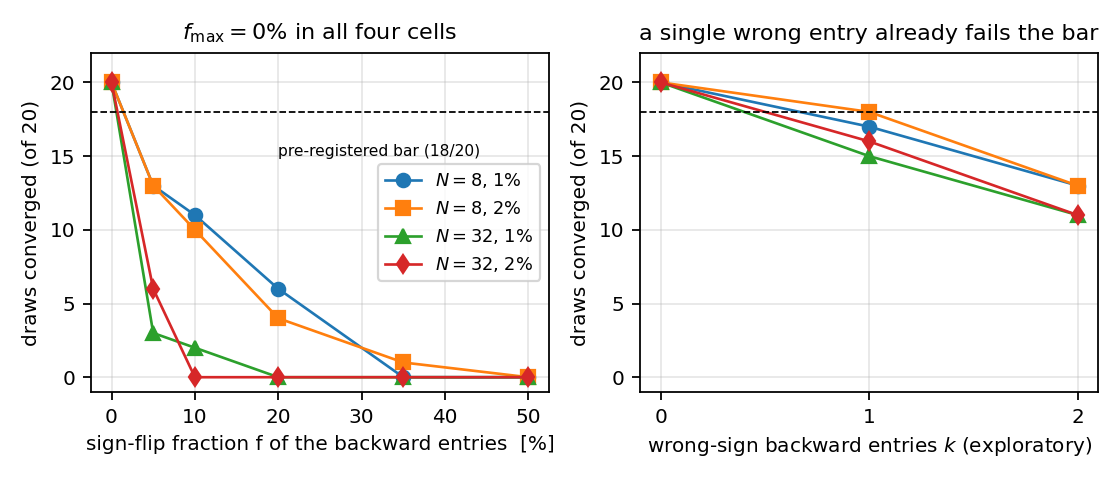
\includegraphics[width=0.92\textwidth]{fig_v3_signflip.png}
\caption{The sign requirement is a hard threshold, not a rate. \textbf{Left}: draws converging to within $2\times$ the exact-adjoint anchor, against the fraction $f$ of backward entries whose sign is flipped; the flip sets are nested, so the curve is monotone in the flipped set. \textbf{Right}: an exploratory refinement with exactly one and exactly two flipped entries (of 32 at $N=8$, of 128 at $N=32$). A single wrong entry already drops convergence below the pre-registered bar in 3 of 4 cells.}
\label{fig:signflip}
\end{figure}

\textbf{Test~S1 (replication).} Criterion: the sign-concordant condition must match the exact-adjoint anchor within $25\%$ on the per-channel median in at least 3 of 4 cells, or the result was a seed artefact. Measured deviation: $\mathbf{0.59\% / 1.14\% / 4.57\% / 9.28\%}$---within $25\%$ in 4 of 4 cells, with \textbf{0 of 80} divergences, sitting on the analytic least-squares floor in every cell. The result replicates; it is no longer exploratory.

\textbf{Test~S2 (magnitude tolerance).} Backward magnitudes drawn log-uniform over a full decade ($0.1$--$1\times$ the true magnitude) \textit{and} a $20\%$ per-channel backward gain mismatch: deviation $\mathbf{0.06\% / 0.67\% / 1.68\% / 1.07\%}$, 4 of 4 cells, 0 of 80 divergences. \textbf{The claim stays ``signs only''.} Backward magnitudes may be wrong by a decade and the backward gain by a fifth, at no measurable cost.

\textbf{Test~S3 (how many sign errors are tolerable).} The pre-registered output is $f_{\max}$, the largest sign-flip fraction at which at least 18 of 20 draws still converge. Measured: $\mathbf{f_{\max} = 0\%}$ in all four cells (Figure~\ref{fig:signflip}). The residual does not degrade gracefully---it sits on the anchor at $f=0$ and is $10^2$--$10^3\times$ the anchor as soon as a channel's sign flips---and the mechanism is deterministic: over the 400 (draw $\times$ $f>0$) records, \textbf{0 of 327} with at least one wrong-sign channel converged and \textbf{69 of 73} with all channel signs correct did. The tolerable \textit{fraction} shrinks as the array grows, since a channel's sign is the sign of a sum of $M$ entries and $P(\text{no channel flips}) \approx (1-q(f))^N$, while the tolerable \textit{count} is zero at every $N$: an exploratory refinement with exactly one flipped entry of 32 (or of 128) already falls below the bar in 3 of 4 cells.

\textbf{Test~S4 (does a non-diagonal stage rescue feedback alignment?).} The prediction being tested was this paper's own: that alignment should return once the trainable stage is a dense matrix that can rotate. Criterion: convergence to within $2\times$ the anchor on the \textit{output} residual in at least 18 of 20 draws, at the better of two learning-rate schedules. Measured: $\mathbf{0/20, 0/20, 0/20, 2/20}$, with an output residual of $161$--$212\%$ against $0.05$--$0.21\%$ for the anchor, while the positive control---the same dense parametrization trained with the exact adjoint---converges $\mathbf{20/20}$ in all four cells. \textbf{The prediction was wrong, and the diagnostic says why.} In the original setting the matrix that rotates towards the random backward path is the \textit{downstream} weight matrix, which is learned; here that matrix is the frozen analog crossbar---the whole point of the mapping---so nothing can rotate. What is left is a linear dynamics stable only if every eigenvalue of $WB^{\mathsf T}$ has positive real part, which for a random $B$ holds in \textbf{2 of 80} draws---and \textbf{S4 converged in exactly those 2 draws and no others: agreement 80/80}. The same obstruction thus appears at both parametrizations, as $\mathrm{diag}(B^{\mathsf T}W)_i > 0$ per channel or $\mathrm{Re}\,\lambda(WB^{\mathsf T}) > 0$ per eigenvalue: \textbf{it lives in the frozen forward matrix's relation to the backward one, not in the trainable stage.}

\paragraph{Consolidated statement.} Reciprocity is \textit{not} required: a separate backward array whose magnitudes are wrong by up to a decade and whose gain is mismatched by $20\%$ trains as well as the exact adjoint. Sign agreement \textit{is} required, exactly. Therefore \textbf{the backward crossbar must share polarity with the forward one at the device level}---a shared sign bit per synapse, or a differential pair written by the same programming operation---while its conductance magnitudes may be left uncalibrated.

\textit{Limitations.} One trainable stage, no depth, $M = 4$; the eigenvalue statistic is $M$-specific, and the direction of the conclusion is robust where the exact $2/80$ is not. What is killed is the mapping claim for a \textit{frozen} analog crossbar, not the original feedback-alignment result, which concerns learned downstream matrices. The sign-flip model is entry-wise independent; correlated polarity errors would be \textit{worse}, since they flip whole channels deterministically. A very small step size would let a wrong-sign channel stall rather than run away, but cannot make it descend---the sign of the averaged update is step-size independent.

\subsection{The cost of needing no backward path at all}
\label{sec:pertcost}

Condition~D removes the sign problem entirely: it has no backward path, needs nothing structural, and reaches the same floor as the exact-gradient condition. Its cost is the question. The first measurement compared two values of $N$ on a budget ladder quantized in factors of 2 and reported ``cost growing roughly $\propto N$''. That inference was unsafe, and a pre-registered re-measurement over \textbf{four} values of $N$, with the ladder extended downward as well as upward and the crossing budget interpolated log-linearly rather than read off a rung, says so.

\begin{center}
\footnotesize
\begin{tabular}{rccccc}
\toprule
$N$ & untrained & B & D & cost ratio D/B (interp.) & converged \\
\midrule
8 & $0.793\%$ & $0.162\%$ & $0.153\%$ & $\mathbf{4.46}$ & 10/10 \\
32 & $0.893\%$ & $0.0568\%$ & $0.0604\%$ & $16.75$ & 10/10 \\
128 & $0.991\%$ & $0.0249\%$ & $0.0280\%$ & $210.5$ & 10/10 \\
512 & $0.993\%$ & $0.0238\%$ & $1.623\%$ & \textbf{never} & \textbf{0/10} \\
\bottomrule
\end{tabular}
\end{center}

Criterion: the fitted exponent $p$ in $\log(\mathrm{D/B}) = a + p\log N$ must lie in $[0.7, 1.3]$, or the earlier ``$\propto N$'' statement is wrong. \textbf{Measured $p = 1.390$ ($R^2 = 0.968$), and the criterion fires.} At a fixed step size the cost grows as ${\approx}N^{1.4}$ and then stops working entirely: at $N = 512$ the perturbative route never reaches exact-gradient quality at any budget on the ladder, up to $1.02\times10^8$ forward evaluations, $100\times$ B's own cost. This is an instability, not a budget statement---the ladder is non-monotone, the residual rising to tens of percent at intermediate budgets before recovering at $N=128$---because the perturbative gradient estimate has variance $\propto N$, so a step size tuned at $N = 8$ is too large at $N \ge 128$. \textbf{The $\propto N$ law is recovered only if the step size is annealed with $N$}: a post-hoc best-of-two-schedules arm gives $p = \mathbf{0.974}$ ($R^2 = 0.927$) across all four $N$ including 512. A second correction falls out of the same re-measurement: the earlier $\mathrm{D/B} = 12.5\times$ at $N = 8$ was \textbf{left-censored}---both conditions already reached the target at the \textit{first} rung of the old ladder, so the ratio measured the ladder, not the algorithms. The true value at $N=8$ is $\mathbf{4.5\times}$; the $N=32$ value reproduces.

\textit{Limitations.} Ten draws per cell and a two-point step-size sweep; the annealed exponent is the best of two step sizes, not of a tuned schedule, and a finer sweep could lower it further. The $N=512$ cell of that arm converges in 8 of 10 draws, so its cost is a slight underestimate of the worst case. Both the second step-size arm and the regularizer of \S\ref{sec:gelulimit} are post-hoc and decide no pre-registered verdict; both should be re-run as pre-registered tests before being relied on.

\subsection{The limit of the mechanism: absorbable means ``in the span of the parameters''}
\label{sec:gelulimit}

The mismatch calculus (\S\ref{sec:calculus}) closed with a design consequence stated as an assertion: the GELU stage's $8.5\%$ per-channel error is dominated by a \textit{static} sigmoid offset, so rule R9 says training can eat it. That was untested, and it is \textbf{false as written}.

The same five conditions were run on the GELU stage (P11$\cdot$P6), with the trainable element extended to a per-channel affine $\gamma_i h_i + \beta_i$---the natural analogue. Criterion: condition~B must bring the per-channel residual below $0.25\times$ its untrained value, computed from this harness's own untrained number. Measured: $\mathbf{0.395\times}$ at $N=8$ and $\mathbf{0.318\times}$ at $N=32$ (from $11.078\%$ to $4.376\%$, and from $13.761\%$ to $4.376\%$), and---decisively---the \textbf{analytic least-squares floor}, the best per-channel affine that exists, is $3.881\%$ ($0.350\times$) and $4.400\%$ ($0.320\times$), also above threshold. Pushing the trained parameters through the real circuit netlist gives $0.509\times$ and $0.309\times$. \textbf{The criterion fires on the surrogate, at the analytic floor, and in simulation.}

The component attribution says which mechanism survives, fitting the optimal affine with one mechanism group active at a time:

\begin{center}
\footnotesize
\begin{tabular}{llcc}
\toprule
mechanism group & rule & absorbed, $N=8$ & absorbed, $N=32$ \\
\midrule
per-channel mirror/VGA gains & R3 & $93.5\%$ & $87.5\%$ \\
translinear \textit{constant} log-gain & R1 ($\iota$) & $97.9\%$ & $95.8\%$ \\
translinear \textit{slope} ($\propto \ln I$) & R1 ($\nu$) & $96.6\%$ & $97.2\%$ \\
\textbf{sigmoid input-referred offset} & \textbf{R12} & $\mathbf{28.6\%}$ & $\mathbf{26.1\%}$ \\
\bottomrule
\end{tabular}
\end{center}

\textbf{``Static'' is necessary but not sufficient. An error is absorbable only if it lies in the span of the trainable parameters.} A per-channel affine absorbs the component of the error in $\mathrm{span}\{h^0(x), 1\}$ over the input distribution. To first order the mismatched stage is $h_i \approx (1+g_i)\,x\,\sigma(1.702x + \delta u_i)$, so the error splits into $g_i h^0(x)$---exactly $\gamma_i$, absorbable---and $\delta u_i\, x\,\sigma(u)(1-\sigma(u))$, a bump peaking near $|x|\approx1$ and vanishing at both ends, while $h^0 = x\sigma(u)$ grows linearly for $x>0$ and vanishes for $x \ll 0$. The two are close to orthogonal, and adding $\beta$ buys almost nothing over $\gamma$ alone ($3.881$ vs $3.915\%$ at $N=8$): the surviving error is not a constant. The one prediction wrong in the \textit{favourable} direction is instructive---the translinear $\nu$ term, classified as an $x$-dependent slope lever and expected to survive, is absorbed to $97\%$, because the translinear lever is $\ln(I/I_s)\approx23$ while $\ln|x|$ varies by only $3.2$ over the input range, so $\nu L$ is ${\sim}93\%$ a constant log-gain.

\textbf{Design consequence, replacing the assertion.} Of the $8.5$--$13.8\%$ per-channel GELU error, roughly \textbf{two thirds is learnable} by a per-channel affine and \textbf{one third---the sigmoid pair's input offset---is not}. Such a stage therefore needs offset cancellation \textit{at the pair} (chopping, autozero, trimming), or a trainable element in the right span: a trainable \textit{input} offset $\sigma(1.702x + b_i)$ would absorb $\delta u$ exactly. Physics-aware training alone leaves ${\approx}4$--$5\%$. Sign concordance is sufficient for this stage too ($0.95$--$1.08\times$ the exact-adjoint condition even with a $20\%$ backward gain mismatch), a second independent confirmation of \S\ref{sec:signconc}.

A practical identifiability rule falls out of the same run. The backward-free condition reaches the \textit{same task loss} as the exact-gradient one to three digits while its per-channel residual explodes to $77$--$80\%$, with the entire additive offset lying in the null space of the frozen read-out: $\beta$ enters the loss only through $W\beta$, $\mathrm{null}(W)$ has dimension $N-M$, and any component there is invisible to every loss-based method. Gradient conditions are protected by construction because their update lies in the row space; a backward-free estimator random-walks. A small decay on $\beta$---physically just leakage of an analog offset store---restores it. \textbf{A trainable additive offset in an analog stage must be regularized or measured, because the task loss does not determine it}, and two parameter sets with identical task loss can differ twentyfold in per-channel residual.

\subsection{Circuit verification and limitations}

The trained parameters were pushed through the \textbf{real junction-exact loop}, with the equilibrium found by bisection on the simulated detector output, for an ideal and a MOS-typical detector. The trivial check must not be over-read: the loop gain is a \textit{scalar} and the metric divides out a best-fit common factor, so any scalar gain gives the identical per-channel number and the $0.000\%$ agreement there is structural. The informative checks are (i)~the loop gain itself, where the simulated junction-exact equilibrium agrees with the surrogate to $\mathbf{0.003}$--$\mathbf{0.006\%}$, i.e.\ the bisected equilibrium \textit{is} $\Gamma/\mathrm{RMS}(x(1+\varepsilon))$ to five digits; (ii)~the \textit{total} error with no common-mode removal, which training cuts from $0.63/1.60/0.95/1.89\%$ to $0.26/0.47/0.14/0.49\%$, so the trained parameters survive the real loop; and (iii)~the MOS detector corner, where the gain shifts by $1.4$--$4.2\%$ and that shift dominates the total error essentially unchanged by training---confirming that detector mismatch is a pure common-mode term, which a static per-channel gain neither can nor should absorb and which the next stage's gain removes in a full network. On the GELU stage, where no loop pins a scalar and the comparison is therefore \textit{not} scale-degenerate, simulated and surrogate per-channel residuals agree to $1$--$2\%$ before training and $16$--$18\%$ after---inside the pre-registered $20\%$ threshold but only just, for an expected reason: once the absorbable part is subtracted, what remains is of the same order as the per-draw difference between a first-order algebra and an exactly solved netlist.

\textit{Limitations of \S\ref{sec:training}.} In this testbench the VGA array is evaluated numerically and only the detector is inside the circuit simulator, so the simulation validates the loop equilibrium and the common-mode/per-channel split, \textit{not} the per-channel VGA path; a per-channel-exact test needs a netlist that does not exist here. One trainable stage, a static graph, a $4\times N$ frozen read-out, no depth, and targets from the ideal network, so the task is exactly ``undo the mismatch''. Thermal noise enters only as $0.5\%$ multiplicative output noise during training; no flicker noise, no drift, no temperature sweep. Device mismatch is fixed per draw, so nothing here says how often a physically trained parameter must be re-learned. All three working routes stop at the analytic least-squares floor set by a 2000-sample training set---the floor, not the gradient source, limits the final number. Finally, condition~B has a heavy upper tail at $N=8$ on the GELU stage (7 of 20 draws flagged) from near-singularity of the system identifying $\gamma$ at $M=4$; the verdict rests on the median and the analytic floor, neither of which has that tail, but the \textit{reliability} of physics-aware training at small $N$ is worse than the median suggests.

\section{Case Results}
\label{sec:cases}

This section reports the circuit-level results behind seven of the reclassified entries of Table~\ref{tab:reclass}. Each was run as a pre-registered test with a numerical kill criterion fixed in writing beforehand; where a criterion fired, it fired as designed and the entry was rewritten rather than quietly kept.

\subsection{Mamba: a selective SSM is a variable-$\tau$ RC cell, not a topology change}
\label{sec:mamba}

Version~2 factorized Mamba's selective state-space model as requiring dynamic topology. The reference algorithm says otherwise: $A$ is a learned parameter and only $\Delta$, $B$ and $C$ are input-dependent~\cite{gu2023mamba}, and a data-dependent gain on a state is a variable$\times$variable multiplication (P11), not a change of wiring. Concretely, $C\,dh/dt = -g_{\mathrm{leak}}(x)h + g_{\mathrm{in}}(x)x$ is $dh/dt = Ah + B(x)x$ with $A_{\mathrm{eff}} = -g_{\mathrm{leak}}/C$; holding the conductances constant over a token slot integrates exactly, and matching against the zero-order-hold discretization gives $g_{\mathrm{leak}} = |A|C\Delta_t/T_{\mathrm{tok}}$, $g_{\mathrm{in}} = C\Delta_t B_t/T_{\mathrm{tok}}$. Criterion~1: if with ideal devices the circuit cannot track the discrete recurrence to $\le1\%$ relative RMS (${\approx}7$ effective bits) over $\Delta\in[0.001,1]$, the P11 factorization is killed---and the report must say whether the failure is device nonlinearity or a discretization mismatch.

\textbf{Criterion~1 not triggered} (Figure~\ref{fig:mamba})\textbf{.} The differential-pair realization reproduces the recurrence to $0.015$--$0.211\%$ (\textbf{8.9--12.7 effective bits}) on 6 of 6 cells; the triode realization reaches $0.0004$--$0.524\%$ on 5 of 6 (up to 18 bits) and misses at $1.066\%$ on the sixth. The miss is attributable, and to neither candidate: not triode \textit{nonlinearity}, which is identically zero in this device model with a pinned common mode (verified to $2\times10^{-7}$), and not the discretization, but \textbf{device-region exit} under a large $\Delta$ dynamic range---shrinking the state swing removes it ($1.066\% \to 0.018\%$). The law behind it is R11: for a triode resistor spanning $R = \Delta_{\max}/\Delta_{\min}$, the state swing is bounded by $2V_{ov,\max}/R$ \textit{and} the control margin by $V_{ov,\max}/R$, two walls closing at once while the mismatch fighting the control margin does not shrink with them. Criterion~3 (selectivity) is likewise not triggered: retention over a hold window is $0.894/0.639/0.167$ for $A=-1/-4/-16$, matched to $0.1$--$1.2\%$ with erasure complete. Selectivity is a voltage on a gate; nothing is routed.

\textbf{Criterion~2 fires---a kill of the naive circuit, not of the factorization}, as pre-registered. Under $\pm3\%$ $K'$ and $\pm10$~mV $V_t$ the median error exceeds $8\%$ in 5 of 9 triode cells ($8.99$--$18.79\%$) and in 9 of 9 pair cells ($\mathbf{723}$--$\mathbf{2122\%}$). The reason is R10: a triode resistor is \textit{two-terminal}, so threshold mismatch is a conductance error and never an offset, whereas a transconductor pair is \textit{three-terminal} and its input-referred offset relaxes the state to $-V_{os}$ and injects a phantom drive---on a 4~mV swing, a 10~mV offset is 2.5 full scales. \textbf{Choose the two-terminal element whenever the state is the thing being multiplied.} Two measured qualifications: at $\sigma(V_t) = 1$~mV the triode variant passes everywhere ($2.0$--$4.2\%$), so this circuit needs large devices or trimming rather than a different principle; and the pair variant's mismatch is overwhelmingly a \textit{static reparametrization}---a six-constant refit brings ${\sim}1000\%$ to $5$--$15\%$---which hands it to \S\ref{sec:training} rather than to a feedback topology. \textbf{No feedback form exists, and the reason is structural}: the AGC result works because there is a target to pin, and a selective SSM has none---$h$ \textit{is} the output, and a loop that pinned it would destroy the memory. This is the boundary of the design principle stated as a circuit fact.

\textbf{A bonus finding.} The capacitor performs the zero-order-hold discretization exactly and for free---the RC integrator computes the exact matrix exponential of its own generator---so the ZOH mapping is the \textit{cheap} one physically, while the reference implementation's simplified Euler write path costs up to $|A|\Delta_{\max}$ of extra write-path dynamic range, $160\times$ here.

\begin{figure}[t]
\centering
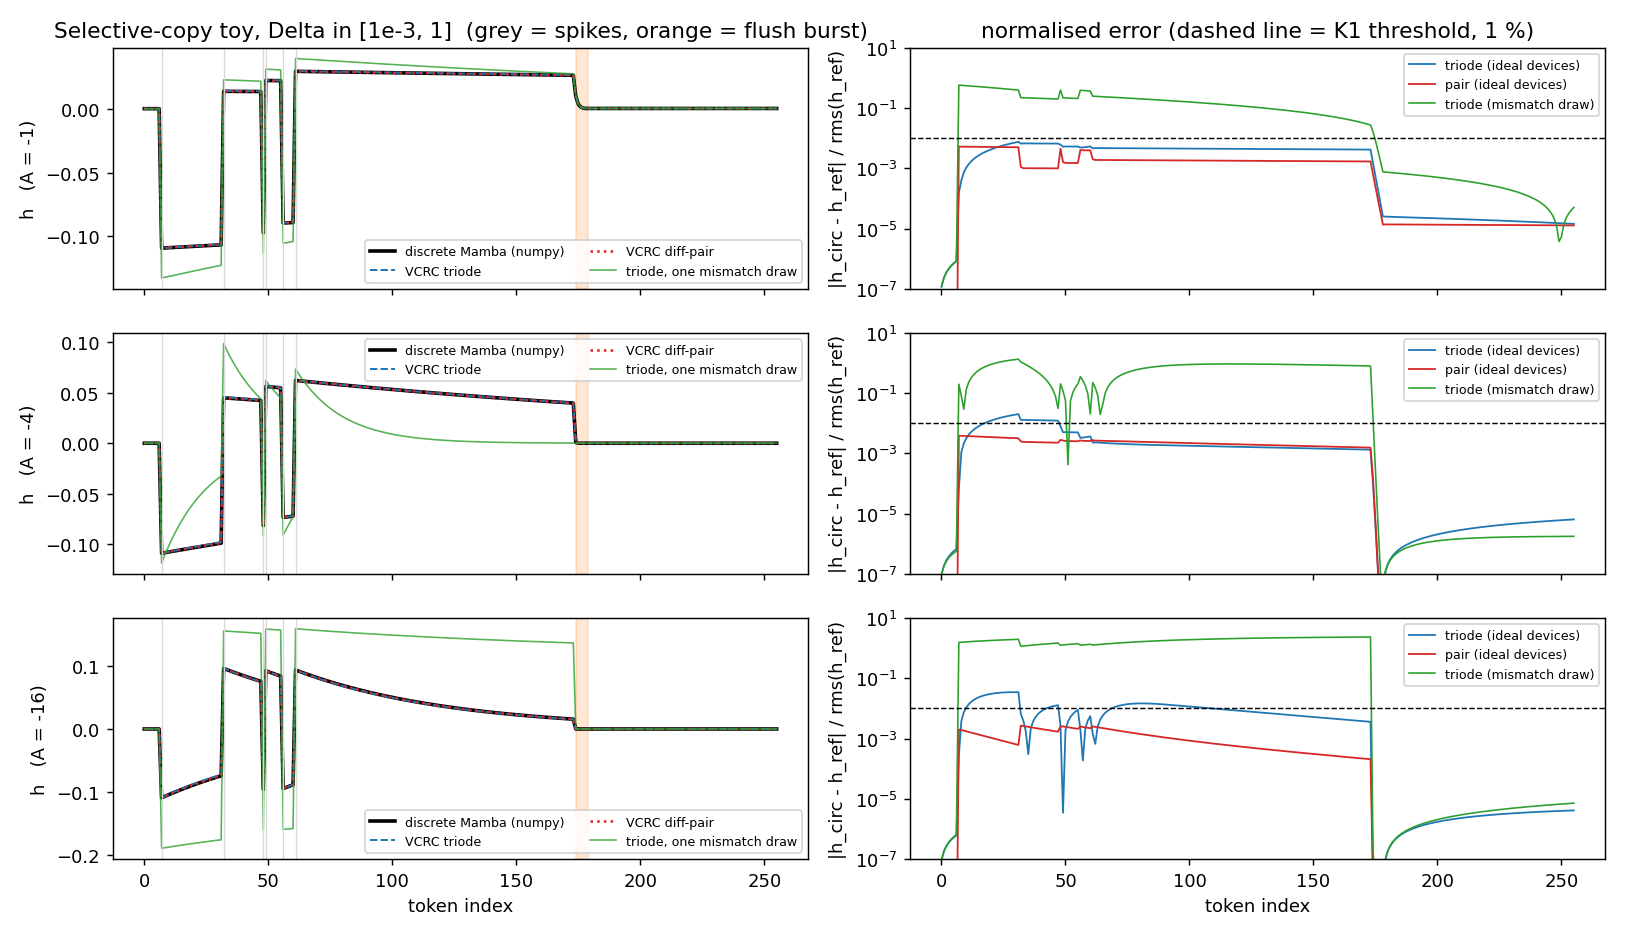
\includegraphics[width=0.96\textwidth]{fig_v3_mamba.png}
\caption{Selective-copy trajectory of the variable-$\tau$ RC realization, $\Delta \in [10^{-3}, 1]$, three channels ($A = -1, -4, -16$). \textbf{Left}: state against the discrete selective-scan reference, for both circuit variants and one mismatched triode draw. \textbf{Right}: normalized per-token error on a log axis, with the $1\%$ criterion marked. Selectivity survives mismatch even where precision does not.}
\label{fig:mamba}
\end{figure}

\textit{Limitations.} The step, the projection and the discretization correction are computed numerically and delivered as ideal control waveforms, so the per-channel converter---its resolution, its mismatch, its settling within a token slot---is not modelled, and five decades of $\Delta$ implies a $\ge$17-bit-equivalent or segmented converter per channel that could easily dominate area and energy. The device model has no weak-inversion region and no short-channel effects, so the exactness of the triode linearity is a property of the model, not of silicon---though the dynamic-range law follows from the triode condition itself. There is no $kT/C$ noise: at 1~pF that is $64\,\mu$V, only ${\sim}36$~dB against the 4~mV swing used here and fatal against the nanovolt swings of the shrunk-swing control. One state dimension, fixed $B_t$, readout projection out of scope.

\subsection{Symbols: a margin, quantitatively---and what the margin costs}
\label{sec:symbol}

Criterion: if the symbol error rate does not fall at least exponentially in $(m/\sigma)^2$---if $\ln\varepsilon$ against $(m/\sigma_{\mathrm{tot}})^2$ is not linear with slope within $30\%$ of $-1/2$ over at least 3 decades---the quantitative X1 row of Table~\ref{tab:assignment} is killed.

\textbf{Not killed.} Over all 48 cells, fitting in the window $z\in[3,6]$---a span of \textbf{6.14 decades} of $\varepsilon$, twice the pre-registered requirement---the slope is $\mathbf{-0.5228}$, a $4.6\%$ deviation from $-1/2$, with simulated and analytic tails agreeing to four digits; the excess is not error but the exact logarithmic correction of the Gaussian tail. A symbol is a margin, quantitatively. A mandatory calibration anchor with a pre-registered stop condition was run first: the classical attractor-memory capacity, reproduced at $0.1460$ at $N = 8000$ ($5.8\%$ off) and $0.1295$ by finite-size extrapolation ($6.2\%$), both inside a $\pm10\%$ band---and, reported honestly, $N\le2000$ alone would have \textit{failed} it.

Four findings beyond the criterion, each of which changes a row of Table~\ref{tab:assignment}.

\textbf{(i)~The feasibility bound, not the margin, binds.} One bit flip moves the score mean by exactly 2 regardless of code width, so the separation between a stored word and its nearest neighbour is \textbf{2 score units at every $k$}, and both sides clear $\varepsilon$ only if $\sigma_{\mathrm{tot}} \le d_{\min}/z_\varepsilon$---a constraint on $\sigma$ alone that no margin setting rescues. At $k=256$ and $\sigma_G = 3\%$ the required margin for $\varepsilon = 10^{-9}$ is \textbf{2.879 units of the 2.0 that exist}; workable instead is $\sigma_G \le 1.04\%$ at $k=256$, or $\mathbf{k \le 30}$ at the $3\%$ corner. \textbf{The fix is code distance, not device quality}: a minimum-distance-8 code at $k=256$ tolerates $8.3\%$, comfortably past the corner, at the cost of alphabet size. That is the honest resolution of the X1 row---its ``digital if'' clause fires for \textit{dense} codes over large alphabets. Thermal noise caps $k$ independently: $k_{\max} = 33/17/8$ at $0.5/1/2\%$ relative match-line noise for $\varepsilon = 10^{-9}$.

\textbf{(ii)~A missing column: match-line gain accuracy.} A fractional gain error $g$ shifts the score mean by $g\cdot k$, and $k/\sigma_{\mathrm{tot}}$ is enormous: $d\ln\varepsilon/dg = 3283$ at $k=256$, $\sigma_G = 3\%$, $\varepsilon = 10^{-9}$, so holding $\varepsilon$ within $2\times$ needs \textbf{10--14 bits} of transimpedance gain accuracy at $k = 64\ldots256$. This is a \textit{systematic}, calibratable error rather than mismatch, which is exactly why no mismatch budget implies it. It is not theoretical: in the circuit check a finite amplifier gain produced a $0.170\%$ score error---predicted to four digits---and that one part in six hundred moved the false-accept count by $15$--$30\%$.

\textbf{(iii)~Retention is a function of load, not a device constant.} Escape times from an attractor state are Arrhenius ($R^2 = 0.88$--$0.94$) with a barrier of \textbf{14.12} at load $\alpha = 0.05$ and \textbf{4.01} at $\alpha = 0.10$: it shrinks $3.5\times$ as the load doubles, so the familiar ``$\Delta E \approx 60\,kT \Rightarrow$ symbol'' reading is right for an \textit{isolated} bistable and wrong for a loaded array. Conversely the feedback (attractor) form absorbs what the open-loop row cannot---$60\%$ synaptic mismatch costs $6.6\%$ of capacity where the open-loop row already fails at $3\%$---the same mechanism as \S\ref{sec:training}, one level up.

\textbf{(iv)~Energy: the margin is nearly free, the line drive is not.} Since the required margin is $z_\varepsilon\sigma_{\mathrm{tot}}$ and $z_\varepsilon^2 \approx 2\ln(1/\varepsilon)$, the margin energy carries the \textit{same} $\ln(1/\varepsilon)$ as the thermodynamic bound and their ratio is independent of $\varepsilon$: at $k=256$, $\sigma_G=1\%$, one restoration to $\varepsilon = 10^{-9}$ costs 141~zJ against an 86~zJ bound, a factor \textbf{1.6} from the Landauer-class limit. The match line itself costs $CV_{FS}^2 = 10$~fJ regardless: \textbf{$1.17\times10^{5}$ times the bound}. Any energy argument for analog symbols must attack capacitance and swing, never the noise margin---and note the tension with (i), since the margin energy per restoration \textit{falls} with $k$ while the feasibility bound \textit{forbids} wide rows, with code distance reconciling them.

Two smaller results. A prefactor criterion fired as a design correction rather than a kill: physical (lognormal) conductance mismatch makes the false-accept tail up to $4\times$ heavier than a Gaussian model at $k\le16$ and $\sigma_G = 5\%$ while making false rejects up to $8\times$ lighter---so the threshold belongs below the symmetric point---and the central limit theorem removes the correction by $k=256$. And under \textit{static} mismatch $\varepsilon$ is a \textbf{yield, not a rate}: at $k=8$, $\sigma_G=3\%$ the fleet mean is $3\times10^{-5}$ while the median row is $3\times10^{-21}$ and the 99.9th-percentile row $2\times10^{-3}$, so per-row trimming or redundancy buys far more than a better average device.

\textit{Limitations.} One row, so row-to-row coupling, match-line loading and sense-amplifier offset are absent---and a CAM with $R$ rows faces $R$ adversaries, a union-bound factor up to $R$ that is not included. Static mismatch only, no read disturb, no compact device model. Thermal noise is a parameter rather than a circuit result, and its parameterization (scaling linearly with $k$) is a modelling choice that makes it dominant at large $k$; an independent-per-line model would scale as $\sqrt k$ and move the $k_{\max}$ numbers upward. The gain-accuracy requirement is analytic plus one circuit confirmation at one operating point, not swept.

\subsection{Bounded recursion: the cost is the write, not the recursion}
\label{sec:recursion}

Two entries that carried X3 were costed with this paper's own transition constants against deliberately favourable digital references. The question was not whether the latency is finite---that is an existence argument---but whether it is \textit{competitive}.

\textbf{Beam search.} Criterion: if the modelled per-step latency at $B=4$, $V = 32768$ exceeds the digital reference by more than $10\times$, the reclassification is hollow---the reference pre-registered at $1\,\mu$s per step, the most accelerator-favourable defensible number. Measured: \textbf{10.18--16.29~ns} per step with capacitive hypothesis slots and serial index readout, $61$--$98\times$ \textit{below} the reference, rising to $1.015\,\mu$s only if every hypothesis copy is a $1\,\mu$s memristive write. Over 64 steps that is $0.65$--$1.04\,\mu$s of beam-specific latency against a 7-billion-parameter model's own ${\sim}15$~ms per token. A second criterion asked whether the ranking is usable: at a selection-boundary gap of 1~nat the top-4 \textit{set} is correct in \textbf{200/200} draws at $N = 64, 256, 1024$. The binding number is the \textit{floor}---$0.203$ correct at $0.25$~nat and $0.000$ at $0.1$~nat at real vocabulary size, so $g_{\mathrm{floor}} \approx 0.5$~nat, below which the compiler must fall back to a digital tie-break. The error budget behind it is R1 in its sharpest form: $3\%$ saturation-current mismatch contributes $0.0300$~nat of effective-logit error while $0.3\%$ ideality mismatch contributes $\mathbf{0.0573}$~nat, because the latter is multiplied by the bias offset $\ln(I_{\max}/I_S) = 19.11$. \textbf{The $0.3\%$ mismatch hurts twice as much as the $3\%$ one}, and worse the harder the devices are biased.

Two laws were verified rather than assumed. The winner's arrival time is \textbf{exactly field-size independent} (1.0000~ns at $N = 64$, 256 and 1024), which is what makes free-slot allocation an $O(1)$ operation, and the $B$-th arrival is $t_{(1)}e^{g_{1B}}$ to $0.002\%$, so readout latency is exponential in the logit gap---a 4-nat gap costs 54.6~ns where a 0.1-nat gap costs 1.1~ns. The energy law $E = V_{dd}CV_{th}Z_{\mathrm{norm}}e^{g_{1B}}$ holds to \textbf{six significant figures}: the race spends its energy on the partition function, not on the field size, which is \textbf{2760--31167$\times$} below digitizing every logit---\textit{but only if the logit path is already analog}. If the scores arrive from a digital matrix multiply, the converters needed to \textit{enter} the race cost nearly what those it saves would, the net saving falls to $2.0\times$, and it is bought with a 131{,}072-cell array. \textbf{The race is a fusion optimization, not a standalone one.}

\textbf{MCTS.} Criterion~A: per-simulation latency must not exceed $10\times$ either of two anchors---a fabricated in-memory MCTS engine at ${\approx}417\,\mu$s per simulation~\cite{molomochir2026}, or a stricter CPU reference at ${\sim}10\,\mu$s. Measured: \textbf{22.0--1078.0~ns} across depth 8--32 and write times of 10~ns--$1\,\mu$s, i.e.\ $9$--$450\times$ under the binding bar. Criterion~B was \textit{designed} to fire, and did: \textbf{the expansion write exceeds $50\%$ of per-simulation time for every write time above 12.0--78.0~ns} (depth 8 parallel to depth 32 sequential); at 100~ns it is $56$--$89\%$ and at $1\,\mu$s $93$--$99\%$. \textbf{The bound that matters is write latency, not recursion depth}, and the entry is renamed B($M$, $d$, $t_{\mathrm{wr}}$). The selection chain is exactly additive at a measured 1.2000~ns per level with \textit{no} accumulation of settling error over 32 levels, and its spread \textit{falls} with depth (coefficient of variation $1.83\% \to 0.94\%$): a deep chain averages its own mismatch. The architectural idea the mapping proposed---a one-hot parallel backup collapsing the $O(d)$ chain to $O(1)$---is worth $8.4$--$37.2$~ns and therefore only matters below a ${\sim}30$~ns write. The interesting idea is the one the dominant cost makes irrelevant. Independent corroboration: the fabricated engine maps expansion to combinational logic and backup to static memory, using the resistive array only for the read-mostly rollout. \textbf{A structural requirement the mapping did not state} is R7: each level's race needs its children's values \textit{as currents}, so the accumulator node and the race driver must be the same physical node, or every simulation re-drives 256 converter channels at 12.8~pJ---the same class of hard precondition as sign concordance in \S\ref{sec:signconc}.

\textit{Limitations.} Mirrors, gating, the winner-take-all threshold and the 200~ps comparator delay are behavioural, and a real winner-take-all over 131{,}072 lines has a fan-in problem this model does not touch. Area is out of scope and is the likeliest real blocker for beam search: 1.311~nF of integration capacitance and 131{,}072 devices for one decode step. The MCTS model excludes the rollout and assumes the selection values already live on the accumulator nodes, so the comparison against the fabricated engine is \textit{not} like-for-like---the defensible statement is narrower, that the phases called ``sequential recursion'' cost tens of nanoseconds and are not where an MCTS accelerator's time goes, which is what that engine's authors say from the other side. Search \textit{quality} is not measured, only ranking correctness and latency spread, and the largest-$N$ beam point is an extrapolation of a law verified at smaller $N$.

\subsection{A remark on which race}
\label{sec:race}

The two P5 realizations are not interchangeable. The race simulated above is the \textbf{deterministic} time-to-threshold race (P3$\cdot$P8$\cdot$P7): arrival times are $CV_{th}/I_i$ exactly, so the ordering is exact by construction and the only error source is device mismatch, measured at 0.0915~nat pairwise. A \textbf{stochastic} race---the thermally activated realization---has per-trial ranking variance. Measured on the exact law: the probability that the first five spikes of a stochastic race are exactly the five highest-rate elements is $3.5\times10^{-5}$ at $N = 1024$, and that they are in the correct order, $4.7\times10^{-7}$; at $k = 10$ and $k = 30$ not one of $6.4\times10^6$ races produced the correct set. Recovering the top-$k$ set by majority vote over repeated races needs $K$ on the order of $10^3$--$10^4$. The information-theoretic version is simulation-free: naming a 5-subset of 1024 costs 43.1 bits and one race supplies 12.8 bits about it. \textbf{For selection---beam search, top-$k$ decoding, mixture-of-experts routing---the deterministic race is the right realization}; its thermal counterpart's spread is 1.81~nat against the deterministic race's 0.0915~nat of mismatch, a factor 20. The stochastic race remains the right realization for what it is good at, namely sampling, where the noise is the product rather than the defect. \textit{Limitation}: this is a statistics-exact, device-ideal computation of the stochastic race law with no device mismatch on top; the two error sources are independent and additive in the log domain, and only the deterministic reference carries mismatch here.

\subsection{KV-cache eviction: the score is free, the selection is not}
\label{sec:kv}

The proposal under test was that a leaky analog cell refreshed by its own read current implements heavy-hitter eviction by physics, with ``no argmin, no scoring logic''. It was tested on real attention traces from a small transformer language model---the forward pass re-implemented from the published weights and verified against the reference to a maximum relative logit deviation of $1.6\times10^{-6}$---in two stages, the second letting the cache policy drive the actual forward pass so that evicted states propagate into all later keys and values.

\textbf{Criterion~1 not killed.} At a cache/sequence ratio of $0.2$ the best leak policy's attention-output error is $90.1\%$ better than a plain sliding window, far past the $20\%$ bar, and \textbf{$28.5\%$ better} than a stronger sink-preserving window added post hoc once plain FIFO turned out to be broken for a known, unrelated reason (it discards the attention sink, which absorbs $38\%$ of the mass in the head measured). \textbf{Criterion~2 not triggered} for the variant with one comparison: against a per-layer-tuned heavy-hitter baseline the leak is $5.1\%$ better, $0.6\%$ better and $11.3\%$ worse at the three budgets. But the overlap with that baseline's retained set is only ${\approx}0.60$ Jaccard---\textbf{leak finds a different, comparably good set}---so ``leak equals the heavy-hitter policy by physics'' is the wrong description.

\textbf{The claim splits in two.} The \textit{scoring} is free: a leaky cell refreshed by its own read current \textit{is} an exponentially discounted accumulated-attention score, needing no counter, adder or comparator to maintain. The \textit{selection} is not: the best configurations sit where the threshold almost never fires (live fraction $0.88$--$1.00$) and one P5 race over the analog charges does the evicting; removing it still beats a sliding window but costs $18$--$49\%$ of attention-output fidelity and $2$--$8\%$ of perplexity. The honest form is \textit{``the score comes from the physics, the selection still costs one P5 race''}, which B($N$) already budgets. The closed loop is the honest metric: with the policy driving the forward pass, perplexity is $37.30$ for a full cache, $41.86$ for the tuned baseline, $44.36$ for the leak, $58.26$ for the sink-preserving window and $2041.7$ for plain FIFO---so in \textit{excess} perplexity the baseline keeps a lead ($+4.57$ against $+7.06$) that the oracle-trace metric did not show.

\textbf{An unanticipated compiler consequence.} Retention must be tied to sequence length. The usable window is ${\approx}32$--$128$ token-times at a sequence length of 512, so a published 5~ms gain cell driven at one token per microsecond is ${\approx}150\times$ too long and degenerates to pure argmin. \textbf{The cell must be made deliberately leakier}---the opposite of the usual retention-engineering direction---and retention becomes a compiler-set parameter tied to the workload rather than a device constant to be maximized. A circuit check confirms realizability: a gain-cell node tracks the difference equation to $0.039\%$ of peak, designed time constant $128.00\,\mu$s against $128.57\,\mu$s measured.

\textit{Limitations.} One model, one dataset, one sequence length, so whether the usable window is absolute or relative to the sequence is \textit{not} determined. Teacher-forced perplexity is not generation quality. The cell simulation is a linear RC with ideal pulses---below this paper's usual fidelity standard---with no transistor, no read disturb, no mismatch and \textbf{no saturation}: the sink cell equilibrates at 18.9~V where a real gain cell saturates near 1~V, and since the one-race variant \textit{reads} the analog value, saturation would degrade the race. One deviation moved the evidence \textit{in favour} of the claim and is flagged: the refresh-strength grid was widened after a first timing run, and the ``one configuration serves every budget'' result depends on it. The baseline was tuned over one hyper-parameter and the leak over a $4\times9$ grid, biasing the comparison in the leak's favour.

\subsection{Three entries that were mapped by argument only}
\label{sec:argentries}

Three reclassified entries named a mechanism without attaching a number. Turning each into a number plus one circuit check produced a result that is the same shape in all three cases: \textbf{``bounded'' is not one bound; it is a bound plus a domain plus a spec.}

\textbf{CTC loss --- the bound tuple must name the signal domain.} One trellis section was built in both the current-log domain (four-junction translinear products) and the charge domain (weight capacitors redistributing onto an output node). Measured per-section error on the log-likelihood channel: $\mathbf{7.862\%}$ in current-log against $\mathbf{0.0128}$--$\mathbf{0.128\%}$ in charge---$614\times$ and $61\times$ quieter---with the calculus prediction within $25\%$ on each component and $10\%$ on the total. Accumulated over 256 sections the log domain crosses the usable 0.1-nat bar \textbf{before the second section} and reaches 1.372~nat spatially unrolled or 19.25~nat time-multiplexed (7.6 / 3.8 effective bits), while the charge domain reaches $0.010$--$0.33$~nat (9.1--14.7 bits). The criterion---log domain above 1~nat \textit{and} the alternative failing too---does not fire, but only because the domain is allowed to change. Cost at 256 sections: 3.4~pJ / $4.2\,\mu$s in log or 6.9~pJ / 256~ns in charge, against 102~pJ of conversion alone to enter a digital forward--backward, a saving that again exists only if the emission stage is already analog; and the sparse recursion the algorithm actually needs uses 4 multipliers per section rather than 16. Two qualifications: the gradient-relevant number is the spread at \textit{fixed} device (0.492~nat), since a per-chip constant offset has zero gradient and is exactly the static class \S\ref{sec:training} absorbs---not claimed here, as no training run was done; and the charge domain's advantage is \textbf{spent by the normalizer}, whose input-referred offset rather than the capacitors becomes binding above ${\approx}17$ sections unless trimmed to ${\approx}1$~mV. \textit{Limitation}: that normalizer was swept analytically and never simulated, and it turned out to be the binding term. One prediction over-predicted by $5.5\times$ and is recorded as a calculus correction: a passive ratiometric charge stage shares capacitors between numerator and denominator, so their mismatch is correlated and cancels to first order, where the pre-registration added them in quadrature.

\textbf{Speculative decoding --- feasible, fast, and it should stay digital.} A dense code of $k = \lceil\log_2 V\rceil$ bits---15 at a 32k vocabulary, 18 at 256k---needs a margin of $0.613$ / $0.676$ of the 2.0 score units available at $\sigma_G = 3\%$, $\varepsilon = 10^{-6}$ per token, union-bounded over the $k$ nearest neighbours; the criterion does not fire, by $3.6\times$. The verify step is 3.764~ns measured end to end, i.e.\ \textbf{1.02~ns per verified token}, and the rollback register is unconditionally free---5 slots held for 18.8~ns need $\ge512$~ns of retention against a measured $128.6\,\mu$s, a $251\times$ margin. \textbf{But mismatch is not the binding term}: with the remaining budget spent on match-line noise the requirement is $\le0.772\%$ relative against the $0.5\%$ already treated as realistic, so the comparator is \textit{noise}-limited with $35\%$ of headroom, and it needs 10.1 bits of transimpedance gain accuracy (R5). \textbf{The energy column settles it}: $42$--$84$~fJ per verified token against ${\sim}1.8$~fJ for a digital comparator tree, a factor $24$--$47$, because an analog comparison must charge a match line to compare two things that are already symbols. \textbf{The comparator is digital-by-position}, for the same reason as the tokenizer and now with a number; what speculative decoding gets from analog is that the draft and target \textit{logits} need no conversion. One free asymmetry: the finite-gain error biases the score \textit{low}, reducing false accepts and increasing false rejects---and a false reject costs one wasted draft token while a false accept corrupts the output. \textbf{Bias the match line low.}

\textbf{Experience replay --- the storage class is forced, not chosen.} The P1 fan-in bound of 256 forces a decoder tree: depth 2 at $10^4$ slots, \textbf{depth 3 at $10^6$}, read latency 1.13 / 1.69~ns. Off-gate leakage follows the junction law to $0.01\%$ over three decades and measures $0.2553\%$ at a 300~mV select overdrive, $1.19\%$ at 260~mV and $12.1\%$ at 200~mV, so the $1\%$ bar needs $\Delta V \ge 262$~mV \textbf{plus 60~mV per decade of slot dynamic range} (322~mV at 10:1, where the 95th percentile otherwise reaches $0.99\%$); mismatch inflates the floor by exactly the predicted $8\%$ and can only make it worse, a sum of exponentials being convex. Compounded over three levels the read is $0.77\%$ systematic plus $1.58\%$ random. The decisive number is the storage class: a $10^6$-slot buffer at 128 cells per slot costs \textbf{1.27~W} of refresh on the measured $128.6\,\mu$s cell, 32.6~mW on a 5~ms cell, and \textbf{$0.128\,\mu$W} on a non-volatile cell written once per environment step---independent of buffer size, because refresh power scales with \textit{capacity} and write power with \textit{throughput}, and a replay buffer is enormous and slowly written. The horizon of seconds to minutes sits $10^3$--$10^6\times$ past that crossover. \textit{Limitation}: endurance and read disturb are not modelled, and the off-gate law is an ideal-junction law, so 262~mV is a floor rather than a design value.

\textbf{Retention is a per-use-site parameter, and the errors point both ways.} The KV cache needs a cell $150\times$ \textit{leakier} than the published one; the rollback register is $251\times$ \textit{over}-specified by that same cell; the replay buffer needs a class it cannot reach at all. Maximizing retention is the wrong default at two of the three sites.

\section{Analysis of Existing Chips}
\label{sec:analysis}

We apply the prime compiler retrospectively to five recent analog accelerators to identify analog mapping opportunities beyond their published partitioning (Table~\ref{tab:chips}).

\begin{table}[t]
\centering
\caption{Retrospective analysis: additional analog mapping opportunities identified by the prime compiler in recent analog chips. The last column notes whether a suggestion is realizable in the chip's existing process or presupposes a device technology not present on the platform.}
\label{tab:chips}
\footnotesize
\begin{tabular}{p{2.8cm}p{2.5cm}p{2.5cm}p{4.5cm}}
\toprule
Chip & Analog / Digital & Compiler suggestion & Additional opportunity \\
\midrule
IBM 14nm PCM~\cite{ibm2025} & MatMul analog; Softmax, Norm, GELU digital & Move GELU (P11$\cdot$P6) and RMSNorm (AGC) to analog & ${\sim}100\%$ of GELU + Norm op energy. AGC is standard-CMOS; GELU demonstrated on RRAM, not yet ported to PCM \\
\midrule
TSMC CIM~\cite{tsmc2025} & MatMul analog; activations digital & Move activations analog; fuse Softmax+Loss (Race) & Activation energy + multi-comp $5\times$. Race fusion requires sMTJ devices---a technology addition \\
\midrule
J\"ulich~\cite{leroux2025a} & QK$^T$ analog; Softmax replaced by HardSigmoid & Use sMTJ Race for exact Softmax & Exact softmax + $5\times$ multi-comp. Requires sMTJ integration---different device technology than the gain-cell platform \\
\midrule
Extropic XTR-0~\cite{extropic2025} & Boltzmann machine analog; digital control & Extract partition fn.\ + entropy from BM relaxation & Class 2.4 multi-comp ($3\times$); readout change on existing hardware \\
\midrule
Normal CN101~\cite{normal2025} & RLC sampling analog; matrix ops digital & Extend to RMSNorm via AGC feedback & On-chip normalization (standard-CMOS AGC); relevant where normalization enters the target workload \\
\bottomrule
\end{tabular}
\end{table}

\textbf{Key finding}: In every chip we analyzed, the compiler identifies nonlinear operations that remained digital but have demonstrated analog mappings. The most common unexploited mapping is GELU (P11$\cdot$P6), which has been demonstrated on RRAM~\cite{rram_swish2022,raceit2023} but was not adopted by any of the five chip teams. The second most common is normalization, which all five teams kept digital---the AGC-based RMSNorm described in \S\ref{sec:rmsnorm}, now validated at circuit level in \S\ref{sec:validation}, resolves this. Notably, the validation also \textit{vindicates} part of the teams' caution: the obvious open-loop translinear approach that a designer would try first is indeed too mismatch-fragile to ship (Table~\ref{tab:mismatch}); the viable path is the feedback topology.

Two caveats bound these findings. First, they are energy-only assessments from published data: area, calibration overhead, testability, and schedule risk---none of which can be evaluated from outside a design team---may well justify the original choices. Second, where a suggestion presupposes a device technology not present on the platform (sMTJ Race on the TSMC and J\"ulich chips; RRAM-demonstrated GELU on the IBM PCM chip), it is a roadmap option, not a missed optimization. The compiler's role is to make the option space and its prerequisites explicit, not to relitigate design decisions.

\subsection{Three design rules}
\label{sec:rules}

The results of \S\ref{sec:domain}--\S\ref{sec:cases} condense into three rules that a mixed-signal team can apply without adopting any of the machinery above.

\textbf{Rule 1 --- Put precision-critical operations inside a feedback equilibrium, and know exactly where the protection stops.} An open-loop realization inherits the full mismatch of every device it traverses, amplified in the log domain by $\ln(I/I_s) \approx 19$--$23$; an equilibrium realization pins the quantity of interest to a loop constraint and demotes device mismatch to a common-mode scale factor that a trained network absorbs. The protection has three measured boundaries. It does not extend \textit{upstream} of the loop input (the exponential stage of a softmax keeps its exposure, which is why feedback wins there by $3\times$ and not by the full junction count). It does not apply where there is \textit{no set-point to pin} (a selective state-space model's state \textit{is} the output, so no loop form exists). And it does not extend \textit{above the loop's own bandwidth}: a per-channel error's transfer to its own output is $1-w_i$ at DC and exactly 1 at high frequency, so a loop demotes a per-channel error by at most $1-1/N$ and demotes nothing at all outside its band.

\textbf{Rule 2 --- Choose the signal domain per operation, and let work flow downstream.} The domain choice moves a number further than the analog/digital choice does---up to 10 effective bits for one prime at one corner. Move the exponential and the logarithm out of current-log into \textbf{time}, where the exponential \textit{is} the axis and no device parameter multiplies it; move inversion into \textbf{feedback} where a set-point exists and into \textbf{time} where none does; move variable multiplication into \textbf{charge} or \textbf{triode} and never into a subthreshold pair; keep accumulation on a wire and integration on a capacitor. Then schedule so that conversions run \textit{into} time and charge---cheap, order-preserving---and never back out into subthreshold current, which re-imports the largest lever in the table. Score levers by \textit{type}, not by size: offset levers are learnable, gain levers trimmable, region-exit neither, and dynamic (noise) levers none of the three.

\textbf{Rule 3 --- Co-locate, and budget the write.} Two preconditions in this paper are structural rather than numerical, and a compiler can only check them, not optimize them away. The accumulator node must \textit{be} the selector drive node, or a selection that should be free costs a full round of conversions per step. And runtime rewiring must be budgeted like a conversion: above a write time of 12--78~ns the mapping is write-bound, and the recursion depth that put the algorithm in the ``unmappable'' column in the first place costs tens of nanoseconds. A fabricated engine independently arrives at the same conclusion by keeping the mutable tree out of the resistive-write path.

\textit{Limitation}: all three rules are stated at the fidelity of \S\ref{sec:validation}--\S\ref{sec:gaps}, with one technology model and no silicon. Rule~1 is the best supported---it has a measured architectural zero, a measured boundary in three directions, and a training-level analogue. Rule~2 rests on lever arithmetic calibrated on one cell with ground truth plus three measured anchors. Rule~3 rests on two cost models with one circuit check each.

\section{Discussion}

\subsection{What the Prime Compiler Does Not Do}

The compiler does not accelerate computation on \textit{existing} digital hardware (CPUs, GPUs). The digital abstraction layer in modern processors seals the underlying transistor physics behind billions of logic gates. There is no software API to operate a GPU's MOSFETs in subthreshold mode.

The compiler's value is in \textit{chip design}: systematically answering the analog/digital partitioning question that every mixed-signal accelerator team faces.

\subsection{Feedback as a Design Principle}

The validation results of \S\ref{sec:validation} suggest a general lesson beyond RMSNorm: \textbf{prefer prime realizations in which precision-critical operations are enforced by feedback equilibrium rather than computed open-loop}. Open-loop translinear arithmetic inherits the full mismatch of every junction it traverses, amplified by the log-domain lever $\ln(I/I_s)$; equilibrium realizations pin the quantity of interest to a loop constraint and demote device mismatch to common-mode error. This distinction is now reflected in the P12 row of the domain-assignment matrix (Table~\ref{tab:assignment}) and should inform the analog mapping of every algorithm in Table~\ref{tab:factorizations} whose factorization contains P12---including Adam's $1/\sqrt{v}$ and any explicit division.

The principle has three measured boundaries, collected in Rule~1 of \S\ref{sec:rules}: feedback protects exactly the operations inside and downstream of the loop, so primes upstream of the loop input retain their per-channel exposure (Result~5); it requires a scalar set-point to exist, which a selective state-space model does not have (\S\ref{sec:mamba}); and it is a DC statement---above the loop's own bandwidth a per-channel error's transfer to its own output is exactly 1, so the noise term of \S\ref{sec:noise} is not demoted at all (rule R19).

It also has an extension, which is the substance of \S\ref{sec:training}. Read one level up, ``pin the quantity of interest by a loop constraint instead of computing it open-loop'' becomes ``measure the gradient on the physical circuit instead of on an idealized model of it''. Both moves have the same effect for the same reason: the error stops being something the design must remove and becomes something the design has already accounted for. The measured version---per-channel residual $0.7$--$0.95\,\sigma \to 0.06$--$0.16\,\sigma$---is the training-level analogue of the architectural zero of Result~4, and the two share a limitation as well as a mechanism, since both demote \textit{static} error and neither touches the dynamic term.

\subsection{The Multi-Computation Advantage}

Multi-computation fusion~\cite{bieg2026} provides $2$--$12\times$ effective throughput multipliers by extracting additional observables from physical events that are already occurring. The prime compiler is, to our knowledge, the first tool to \textit{automatically detect} these opportunities in arbitrary compute graphs.

Without the compiler, fusion opportunities are found (or missed) by manual inspection. With the compiler, every subgraph matching a known multi-computation class is flagged and quantified.

\subsection{Argmax as Three Substrate Requirements}
\label{sec:argmax}

P5 was the one prime the domain-assignment matrix marked ``always physics''. The case results replace that entry with three requirements, each of which a real design can fail. \textbf{(i)~The realization must be the deterministic race}: a thermally activated race and a time-to-threshold race are the same prime in the catalogue and are not interchangeable in a circuit, since the deterministic one orders exactly in one shot with device mismatch as its only error budget while the stochastic one returns the correct top-5 set of 1024 competitors with probability $3.5\times10^{-5}$ per trial (\S\ref{sec:race}). Selection and sampling are different jobs and want different devices. \textbf{(ii)~The accumulator node must be the selector drive node}: argmax is cheap only when the compared quantity is already a current on the node that drives the comparison, and breaking that co-location costs a full round of conversions per step (\S\ref{sec:recursion})---a placement constraint, not a precision one. \textbf{(iii)~A selection-boundary gap must be declared}: the ranking is exact only down to the mismatch of the competing elements, $0.0647$~nat per element and $0.0915$~nat pairwise at the MOS-typical corner, dominated not by the $3\%$ saturation-current spread but by the $0.3\%$ ideality spread times the bias offset, giving a usable floor $g_{\mathrm{floor}} \gtrsim 6\sqrt2\,\sigma_{\mathrm{tot}} \approx 0.5$~nat, below which the compiler must fall back to a digital tie-break. A fourth condition is a placement precondition rather than a substrate requirement, and it recurs: the race pays only if the score path is \textit{already} analog. \textit{Limitation}: (i) and (iii) are measured at the wiring-ideal fidelity level, and a real winner-take-all over $10^5$ lines has a fan-in problem none of these tests touches.

\subsection{What Remains Genuinely Digital}
\label{sec:digital}

Reading X1--X4 as Turing components (\S\ref{sec:missing}) does not make everything analog; it relocates the boundary and makes it quantitative. Four things stay digital, each for a different reason.

\textbf{Exactness}, because it has a thermodynamic price. Restoring a symbol to error rate $\varepsilon$ costs at least ${\sim}kT\ln(1/\varepsilon)$, and \S\ref{sec:symbol} measures the margin at a factor 1.6 from that bound while the \textit{line drive} that delivers it is five orders above. Exactness is not impossible in analog; it is cheap in the margin and expensive in the wire, which is exactly the regime where a digital gate wins. Quantitatively, the X1 row says symbolic operations demand an error rate below what the platform's analog noise margin provides---at the $3\%$ corner, capping a dense code at ${\approx}30$ bits.

\textbf{Unboundedness}, because no physical computer has it, and it is resolved the way every synthesis flow resolves it: the compiler asks for the bound. Nature does not do unbounded recursion either---branching morphogenesis self-terminates at a physical floor and human centre-embedding maxes out near depth three---which is one reason to read X3 as belonging to software.

\textbf{Dynamic control flow}, because that is what a tape is actually for. For a static graph the backward graph is a fixed second circuit known at compile time and the tape reduces to holding activations, which is P8; what survives is the tape for \textit{data-dependent} control flow, for which no verified physical analogue was found and a hybrid digital model remains the state of the art.

\textbf{Token comparison, by position.} Comparing two symbols in analog is feasible, fast ($1.02$~ns per verified token) and accurate enough ($\varepsilon = 10^{-6}$ with a third of the available margin), and it still loses by $24$--$47\times$ on energy to a digital comparator tree because it has to charge a match line to compare two things that are already symbols (\S\ref{sec:argentries}); the tokenizer is the same argument at the input boundary. \textbf{Digital-by-position is a real category}: the operation is mappable and the mapping is pointless, and a compiler that reports only mappability will get this wrong.

\subsection{Towards Training}

On analog-only hardware, v2 treated training as blocked by X4. \S\ref{sec:training} replaces that with a condition and a cost. For a static graph, a gradient is available from any one of three physical families---an adjoint through reciprocal linear parts, an energy-based settle-twice scheme, or a black-box perturbative estimator---and the compiler's job is to check which structural property the target platform actually has. The measured requirements are sharper than the literature's framing suggested in one direction and looser in another: \textbf{reciprocity is not required} (backward magnitudes may be wrong by a decade and the backward gain by $20\%$), but \textbf{sign concordance is}, exactly, which is a statement about how the backward array must be \textit{programmed} rather than about how accurately it must be trimmed. Where no backward array is available at all, the perturbative route works with nothing structural, at a cost of $4.5$--$210\times$ the forward evaluations up to $N = 128$ at a fixed step size---an arm that fits $N^{1.39}$ and then fails to converge at all at $N = 512$---or $2.5$--$116\times$ across $N = 8\ldots512$ once the step size is annealed with the array size, which is the arm that recovers the $N^{0.97}$ law (\S\ref{sec:pertcost}).

The mechanism has a ceiling, and it is not about static versus dynamic error. An error is absorbable if and only if it lies in the \textit{span of the trainable parameters}: the same physics-aware gradient that removes $79$--$94\%$ of the AGC stage's per-channel mismatch removes only $26$--$29\%$ of a sigmoid pair's input-referred offset, because the resulting error shape is close to orthogonal to what a per-channel output affine can express. The design response is to move the trainable element to where the error lives---a trainable input offset rather than a trainable output gain---or to cancel the offset at the device.

\textit{Limitation}: everything in this subsection concerns a single trainable stage in a static graph with targets taken from an ideal reference. It is evidence about a mechanism, not about training a network.

\subsection{Limitations}
\label{sec:limitations}

Collected here, in the order in which they would bite a design team.

\textbf{The mismatch calculus is static, with exactly one dynamic class.} Rules R1--R17 and R21 price static device-parameter spread and a spatial temperature gradient; R18--R20 add \textit{white} device noise. Flicker and random-telegraph noise are absent throughout, are not bandwidth-scalable, and typically dominate below ${\sim}1$~MHz in subthreshold devices, so every noise figure in \S\ref{sec:noise} is a lower bound. Supply noise, substrate noise and channel-to-channel coupling are absent. Slew, large-signal settling and stability margin remain outside the algebra: settling time is an \textit{input} to the cost model, and R20 says only what that input costs.

\textbf{Wiring is ideal, one notch relaxed.} Every exponential current in this paper comes from a real device law, and \S\ref{sec:gaps} adds Early effect, bias-network error, finite integrator gain and capacitor mismatch. But translinear loop wiring is still voltage summation by controlled sources; mirrors, differential copies, comparators and rectifiers carry a \textit{stated} gain error or delay rather than a modelled output impedance, bandwidth, charge injection or base current. In two testbenches the per-channel multiplier array itself is evaluated numerically and only the shared path is simulated, so those runs validate the loop and the common-mode split, not the per-channel path.

\textbf{Mismatch is independent.} No spatial correlation, no shared bias network, no area law. Where the correlated case has been examined it is \textit{worse}, not better: correlated polarity errors flip whole channels deterministically, and a thermal gradient across a large array is perfectly correlated and neither averages nor is demoted. This is an optimistic assumption and it is not tested.

\textbf{One technology model, no PDK, no silicon.} Level-1 device equations, ideal junctions, bipolar stand-ins for subthreshold pairs, microamp biases. The levers $\ln(I/I_s) \approx 19$--$23$ are properties of \textit{these} numbers; on a real process the rules survive and the constants do not. There is no layout, no parasitic extraction, no endurance or read-disturb model, and no measured device. Silicon remains the final arbiter for every number here.

\textbf{Area is out of scope, and is repeatedly the likely real blocker.} A 131{,}072-cell race array is 1.311~nF of integration capacitance; a $10^6$-slot buffer, a 262{,}144-tap match line and a 256-section unrolled trellis are area problems none of the cost models touch. The charge domain's bit advantage is bought with capacitor area, and at femtofarad unit sizes the matching that advantage rests on is ${\sim}1\%$ rather than $0.1\%$.

\textbf{Scope of the training results.} One trainable stage, a static graph, a frozen four-output read-out, no depth, no non-linearity after the stage, and targets drawn from an ideal reference so that the task is exactly ``undo the mismatch''. The feedback-alignment result is a statement about a \textit{frozen} forward crossbar and says nothing about the setting where the downstream matrices are themselves learned. Two of the conditions reported are post-hoc controls and are labelled as such; both should be re-run as pre-registered tests before being relied on.

\textbf{Nothing here measures task quality.} Ranking correctness, log-likelihood error, comparison error and read fidelity are measured; search quality, training convergence, draft acceptance rate and sample efficiency are not.

\section{Related Work}
\label{sec:related}

\textbf{CIM compilers.} CIM-MLC~\cite{cimmlc2024} provides a multi-level compiler for compute-in-memory accelerators (ASPLOS 2024), and CINM~\cite{cinm2024} generalizes across CIM and CNM paradigms via MLIR. CMSwitch~\cite{cmswitch2025} jointly optimizes compute-mode and memory-mode switching in CIM arrays. All three treat CIM arrays as ``noisy MAC units'' and route everything else to digital---none decompose operations into analog-native primitives or reason about \textit{which} operations beyond MAC are physically suited to analog.

\textbf{Hybrid analog-digital SoCs.} DIANA~\cite{diana2022} integrates analog CIM and digital accelerators on one SoC; its compiler HTVM~\cite{htvm2023} dispatches layers to either domain based on hardware capability matching, not operation semantics. The IBM mixed-precision supernetwork~\cite{ibm_supernetwork2026} uses NAS to find layer-to-hardware assignments---the closest existing work to systematic partitioning, but empirical (search-based) rather than principled (decomposition-based). A 2025 framework for DNN inference partitioning in hybrid analog-digital chiplets~\cite{hybrid_partition2024} operates at layer granularity with accuracy-vs-energy tradeoffs.

\textbf{Analog compilers.} Legno~\cite{legno2020} compiles differential equations to reconfigurable analog devices, mapping physics to computation---the closest precedent to our approach. Hasler's FPAA toolflow~\cite{hasler2020} programs floating-gate analog arrays from high-level descriptions. Both target analog-only execution of general computations; neither addresses the analog/digital partitioning problem for neural networks.

\textbf{DNN compilers.} TVM, XLA, and \texttt{torch.compile} partition across digital hardware types (CPU/GPU/TPU) but not across physical domains. NIR~\cite{nir2024} defines a neuromorphic intermediate representation for spiking systems across 7 simulators and 4 hardware platforms, but targets spike-based computing, not analog/digital CIM partitioning.

\textbf{Analog simulation.} NeuroSim~\cite{neurosim}, CrossSim~\cite{crosssim}, and IBM's AIHWKIT~\cite{aihwkit2023} simulate analog non-idealities for accuracy estimation. NavCim~\cite{navcim2024} performs design-space exploration for CIM architectures. None factorize operations into primes or detect multi-computation opportunities. Our validation methodology (\S\ref{sec:validation}) is complementary: it operates at the junction-physics level of a single mapped operation rather than at network-accuracy level.

\textbf{Normalization in analog.} IMPACT~\cite{impact2023} implements batch normalization as a linear gain and offset in the ADC, i.e.\ a pre-computed affine transform rather than true normalization. The ReRAM ALN~\cite{reram_aln2022} normalizes in the charge domain, with simplifications. Yang et al.~\cite{yang2022} go furthest: their full-circuit memristor transformer implements Layer Normalization as one of five analog function-circuit modules and completes every calculation on the analog signal without ADC, DAC or digital memory, verified in PSPICE---so an analog LayerNorm block is prior art, and we distinguish our contribution from it not by feasibility but by mechanism: their module computes the normalization forward through dedicated function circuits, whereas \S\ref{sec:agc} obtains it as the equilibrium of a gain loop, which is what makes the mismatch result of \S\ref{sec:validation} possible (their published abstract does not state whether the module evaluates $1/\sqrt{\mathrm{var}}$ explicitly or approximates it, and the paper is paywalled). We found no analog RMSNorm in the literature. The AGC circuit family itself is classical~\cite{gilbert1975,pelgrom1989}; its identity with RMSNorm, and the mismatch analysis of that identity, are new here.

\textbf{Analog compilation and the signal domain.} Beyond Legno~\cite{legno2020}, Ark~\cite{ark2024} provides a language for \textit{describing} an analog compute paradigm with a validator and compiler, and Shem~\cite{shem2024} optimizes hardware parameters by differentiating through time-domain simulation with noise and mismatch. In all three the signal domain is fixed before compilation begins. The closest work to \S\ref{sec:domain} is Freye et al.~\cite{freye2024}, comparing time-domain, charge-domain analog and digital vector--matrix multiplication quantitatively---but per macro for one fixed workload, not as a per-operation synthesis decision; charge-versus-current is likewise a well-made design argument~\cite{capram2021,valavi2019}. We found no published framework treating the signal domain as a per-operation compile-time choice with a mismatch-lever cost model.

\textbf{Physical gradients.} Reverse-mode sensitivity was established in circuit theory in 1969, from one adjoint network run~\cite{director1969}; the crossbar version is explicit---driving the columns computes the transpose product~\cite{gokmen2016}---and the adjoint field has been obtained physically with the gradient measured in situ~\cite{hughes2018}, the strongest single counterexample to treating symbolic tracing as a missing prime. Equilibrium propagation~\cite{scellier2017} and its realizations in resistor networks~\cite{dillavou2022} and Ising machines~\cite{laydevant2024} obtain the gradient by settling twice; time-reversal schemes~\cite{lopezpastor2023} pay in reversibility; zero-order routes measure it on the network itself~\cite{cauwenberghs1996,baydin2022,leblanc1922,krstic2000}; and Wright et al.~\cite{wright2022} make the mismatch argument with a hybrid digital backward model. Against this background our contribution is narrow: we measure which structural property is load-bearing for a \textit{frozen} analog forward crossbar, and find that reciprocity is not, sign symmetry~\cite{liao2016,xiao2018} is, and feedback alignment~\cite{lillicrap2016}---together with the weight-mirror and Kolen--Pollack routes that learn the backward matrix without transporting weights~\cite{akrout2019}, which a frozen forward crossbar cannot run---is unavailable at either parametrization---not because alignment is wrong, but because the matrix that would have to rotate is the one held fixed.

\textbf{Symbolic operations in analog hardware.} Analog content-addressable memories perform exact and range matching over all rows in one step~\cite{li2020acam}, tree-based inference has been run in memristive analog CAM~\cite{pedretti2021}, and a memristive ternary CAM executes regular-expression finite-state machines and a Levenshtein automaton~\cite{graves2020tcam}, which bears directly on the claim that regular-expression matching has no physical mapping; automata processing in memory has a commercial precedent~\cite{dlugosch2014}. Hashing as random projection plus winner-take-all, and set membership as its Bloom-filter analogue, are established in the neuroscience literature~\cite{dasgupta2017,dasgupta2018}. Sort-in-memory~\cite{yu2025sort} bears on the \texttt{sort} entry of Table~\ref{tab:reclass}, a multi-primitive in-memory tree-search engine~\cite{molomochir2026} on the MCTS entry, and trellis forward--backward processing---the recursion underlying CTC---was built in subthreshold analog VLSI as a direct sum-product implementation~\cite{loeliger2001}. Collectively these establish that every ``no physical implementation'' entry of the v2 table has at least one published counterexample, the single exception being a subword tokenizer, which is unbuilt rather than impossible and sits at the digital input boundary anyway.

\textbf{Key gap.} No existing framework operates at \textit{operation granularity} with a \textit{principled decomposition} into analog-native primitives, a \textit{per-operation domain choice}, and a \textit{composable mismatch budget}. All partitioning decisions in the literature are either (a)~layer-level, (b)~hardware-capability-driven, or (c)~empirical search; all analog compilers fix the signal domain before they begin; and all mismatch analysis is per-circuit Monte-Carlo simulation rather than per-prime characterization plus composition. The prime compiler provides a theory-driven, operation-level partitioning framework grounded in physics, and \S\ref{sec:calculus} carries a mismatch budget per prime the way a synthesis tool carries a timing budget per cell; budgeting and sensitivity analysis have a long history in analog design automation, and what we claim as new is only their placement at the level of primes and signal domains, ahead of any topology.

\section{Conclusion}

We have introduced Computational Primes---12 irreducible operations with physical implementations and 4 without---as a systematic basis for decomposing neural network computation. The resulting prime compiler automates the analog/digital partitioning problem that every mixed-signal accelerator team currently solves by hand.

Key results:
\begin{itemize}[leftmargin=*]
\item \textbf{114 algorithms factorized: 93 analog-mappable, 20 bounded-mappable, 1 digital-by-position, 0 fundamentally unmappable.} The four ``missing primes'' are the four components a finite circuit lacks relative to a Turing machine, so the line they mark is the circuit/software line rather than the analog/digital line, and every synthesis flow meets it in the same place. What survives as genuinely unmappable is unboundedness itself, exactness itself, dynamic control flow, and---on energy rather than feasibility grounds---token comparison at a digital boundary.
\item RMSNorm mapped to analog via AGC feedback and validated in over 17{,}000 SPICE simulations: settling to the exact equilibrium in 4--6~ns with no ADC in the loop; detector-side mismatch produces exactly zero per-channel distortion. The same loop with a sum detector computes softmax, beating the open-loop realization $3.1$--$3.4\times$ under paired mismatch.
\item \textbf{The four open validation gaps are closed}, and closing them corrected three published claims. Four-quadrant signalling preserves the architectural zero at no cost \textit{with class-AB rails}, while class-A costs $1.79\,\sigma_{\mathrm{VGA}}$; $N = 4096$ holds at $1.09\times10^{-7}$ ideal-device error provided the summing node stays at virtual ground and per-channel current is not scaled down; a realistic 60~dB integrator moves loop closure from $10^{-4}$ to $7.2\times10^{-4}$; and thermal/shot noise is a \textbf{third per-channel exposure} obeying $\sigma_{\mathrm{pc}} = 0.78\sqrt{k_j 2qB/I_0}$---equal to the mismatch residual at $I_0 = 1\,\mu$A and $B = 122$~MHz, $3.3\times$ larger at the published loop's actual bandwidth, and restored to the mismatch floor by critically damping the loop at a $1.34\times$ settling cost.
\item \textbf{The design principle extends to training.} A gradient measured on the mismatched circuit reduces the per-channel residual from $0.7$--$0.95\,\sigma$ to $0.06$--$0.16\,\sigma$, exactly the analytic least-squares floor. The backward path needs sign concordance and not reciprocity: magnitudes may be wrong by a decade and the backward gain by $20\%$, but the tolerable number of wrong-sign channels is \textit{zero}, not a small percentage. Feedback alignment is unavailable for a frozen forward crossbar at either parametrization, with the obstruction measured as an eigenvalue condition satisfied in 2 of 80 random draws---and satisfied in exactly the 2 draws that converged.
\item \textbf{The design space is tractable without a simulation per design point.} A signal-domain axis prices the choice below analog-vs-digital, where one prime spans up to 10 effective bits at one corner; and 21 composition rules over a per-prime sensitivity tuple retrodict 36 measured numbers with none outside a factor 2 and predict two unseen composites to $1.00\times$ and $1.05\times$. Circuit simulation becomes an arbiter rather than a characterization tool.
\item Retrospective analysis of 5 chips identifies 15--40\% additional energy savings on nonlinear operations, subject to each platform's device-technology prerequisites, and condenses into three transferable design rules.
\item Multi-computation fusion detected automatically, yielding $2$--$12\times$ throughput---with the caveat that the fusion is a fusion: the race saves conversions only where the score path is already analog.
\end{itemize}

The prime compiler does not make existing GPUs faster. Its value is in chip design methodology: replacing ad hoc partitioning with a systematic, automatable framework. The single result that generalizes furthest is the smallest: \textit{prefer realizations in which the precision-critical quantity is pinned by a constraint the circuit already satisfies, rather than computed by devices the circuit has to trust}---at the level of a normalization loop, and again at the level of the gradient that trains it. As analog accelerators move from research prototypes to production silicon, the need for such a framework will only grow. Silicon remains the final arbiter for every number reported here.

Code, the full factorization table, and the SPICE validation testbenches are available in the code archive attached to this record and at: \url{https://github.com/Biech95/prime-compiler}.

\begin{thebibliography}{99}

\bibitem{ibm2025} A.~Chen \textit{et al.}, ``Demonstration of transformer-based ALBERT model on a 14nm analog AI inference chip,'' \textit{Nature Communications}, 2025.

\bibitem{tsmc2025} W.-S.~Khwa \textit{et al.}, ``A mixed-precision memristor and SRAM compute-in-memory AI processor,'' \textit{Nature}, 2025.

\bibitem{extropic2025} A.~Jelincic \textit{et al.}, ``An efficient probabilistic hardware architecture for diffusion-like models,'' \textit{arXiv:2510.23972}, 2025.

\bibitem{normal2025} D.~Melanson \textit{et al.}, ``Thermodynamic computing system for AI applications,'' \textit{Nature Communications}, vol.~16, 3757, 2025.

\bibitem{leroux2025a} N.~Leroux \textit{et al.}, ``Analog in-memory computing attention mechanism for fast and energy-efficient large language models,'' \textit{Nature Computational Science}, 2025.

\bibitem{bieg2026sba} M.~Bieg, ``Stochastic Barrier Attention: Normalization-free softmax sampling via thermodynamic race processes,'' \textit{Zenodo}, 2026, doi:10.5281/zenodo.19265587.

\bibitem{bieg2026} M.~Bieg, ``Multi-computation from exponential race events: Extracting simultaneous observables from stochastic barrier arrays,'' \textit{Zenodo}, 2026, doi:10.5281/zenodo.19265605.

\bibitem{prezioso2015} M.~Prezioso \textit{et al.}, ``Training and operation of an integrated neuromorphic network based on metal-oxide memristors,'' \textit{Nature}, vol.~521, pp.~61--64, 2015.

\bibitem{sillman2023} J.~Sillman, ``Analog Implementation of the Softmax Function,'' \textit{arXiv:2305.13649}, 2023.

\bibitem{tageldeen2025} M.~K.~Tageldeen \textit{et al.}, ``Learning in log-domain: Subthreshold analog AI accelerator based on stochastic gradient descent,'' \textit{arXiv:2501.13181}, 2025.

\bibitem{mram_sigmoid2022} M.~H.~Amin \textit{et al.}, ``MRAM-based analog sigmoid function for in-memory computing,'' \textit{GLSVLSI}, pp.~319--323, 2022.

\bibitem{denram2024} S.~D'Agostino \textit{et al.}, ``DenRAM: Neuromorphic dendritic architecture with RRAM for efficient temporal processing with delays,'' \textit{Nature Communications}, vol.~15, 2024.

\bibitem{cryptoristor2024} S.-I.~Kim \textit{et al.}, ``Cryptographic transistor for true random number generator with low power consumption,'' \textit{Science Advances}, vol.~10, eadk6042, 2024.

\bibitem{gilbert1975} B.~Gilbert, ``Translinear circuits: A proposed classification,'' \textit{Electronics Letters}, vol.~11, no.~1, pp.~14--16, 1975.

\bibitem{elfadel1993} I.~M.~Elfadel and J.~L.~Wyatt~Jr., ``The `softmax' nonlinearity: Derivation using statistical mechanics and useful properties as a multiterminal analog circuit element,'' \textit{Advances in Neural Information Processing Systems~6 (NIPS)}, 1993.

\bibitem{pelgrom1989} M.~J.~M.~Pelgrom, A.~C.~J.~Duinmaijer, and A.~P.~G.~Welbers, ``Matching properties of MOS transistors,'' \textit{IEEE Journal of Solid-State Circuits}, vol.~24, no.~5, pp.~1433--1439, 1989.

\bibitem{rram_swish2022} A.~Fatima and A.~Pethe, ``Implementation of RRAM based Swish activation function and its derivative on 28nm FD-SOI,'' \textit{Int.\ Electrical Engineering Congress (iEECON)}, pp.~1--4, 2022.

\bibitem{raceit2023} L.~Zhao, A.~Natarajan, L.~Buonanno, A.~Gajjar, R.~M.~Roth, S.~Serebryakov, J.~Moon, J.~Ignowski, and G.~Pedretti, ``RACE-IT: A reconfigurable analog computing engine for in-memory transformer acceleration,'' \textit{arXiv:2312.06532}, v3, 2025.

\bibitem{zhang2026ssm} X.~Zhang, M.~Hu, S.~Lu, S.~Kim, E.~Y.-J.~Lee, Y.~Liu, and W.~D.~Lu, ``Compute-in-memory implementation of state space models for event sequence processing,'' \textit{Nature Communications}, vol.~17, 1513, 2026.

\bibitem{zhang_rmsnorm2019} B.~Zhang and R.~Sennrich, ``Root mean square layer normalization,'' \textit{NeurIPS}, 2019.

\bibitem{carandini2012} M.~Carandini and D.~J.~Heeger, ``Normalization as a canonical neural computation,'' \textit{Nature Reviews Neuroscience}, vol.~13, pp.~51--62, 2012.

\bibitem{neurosim} P.-Y.~Chen \textit{et al.}, ``NeuroSim: A circuit-level macro model for benchmarking neuro-inspired architectures,'' \textit{IEEE TCAD}, 2018.

\bibitem{crosssim} S.~Agarwal \textit{et al.}, ``CrossSim: Accuracy simulation of analog in-memory computing,'' \textit{Sandia National Lab}, 2023.

\bibitem{legno2020} S.~Achour and M.~Rinard, ``Noise-aware dynamical system compilation for analog devices with Legno,'' \textit{ASPLOS}, pp.~149--166, 2020.

\bibitem{hasler2020} J.~Hasler, ``Large-scale field-programmable analog arrays,'' \textit{IEEE Proceedings}, 2020.

\bibitem{impact2023} A.~Kneip \textit{et al.}, ``IMPACT: A 1-to-4b 813-TOPS/W 22nm FD-SOI CIM-SRAM with multi-bit analog batch-normalization,'' \textit{IEEE JSSC}, 2023.

\bibitem{yang2022} C.~Yang, X.~Wang, and Z.~Zeng, ``Full-circuit implementation of transformer network based on memristor,'' \textit{IEEE Trans.\ Circuits Syst.\ I: Regular Papers}, vol.~69, no.~4, pp.~1395--1407, 2022.

\bibitem{reram_aln2022} S.-G.~Gi, H.~Lee, J.~Jang, and B.-G.~Lee, ``A ReRAM-based convolutional neural network accelerator using the analog layer normalization technique,'' \textit{IEEE Trans.\ Industrial Electronics}, vol.~70, pp.~6442--6451, 2023.

\bibitem{cimmlc2024} S.~Qu \textit{et al.}, ``CIM-MLC: A multi-level compilation stack for computing-in-memory accelerators,'' \textit{ASPLOS}, pp.~185--200, 2024.

\bibitem{cinm2024} A.~A.~Khan \textit{et al.}, ``CINM (Cinnamon): A compilation infrastructure for heterogeneous compute in-memory and compute near-memory paradigms,'' \textit{ASPLOS}, pp.~31--46, 2024.

\bibitem{cmswitch2025} S.~Zhao \textit{et al.}, ``Be CIM or Be Memory: A dual-mode-aware DNN compiler for CIM accelerators,'' \textit{ASPLOS}, pp.~63--78, 2025.

\bibitem{diana2022} K.~Ueyoshi \textit{et al.}, ``DIANA: An end-to-end energy-efficient digital and analog hybrid neural network SoC,'' \textit{ISSCC}, 2022.

\bibitem{htvm2023} J.~Van Delm \textit{et al.}, ``HTVM: Efficient neural network deployment on heterogeneous TinyML platforms,'' \textit{DAC}, 2023.

\bibitem{ibm_supernetwork2026} H.~Benmeziane \textit{et al.}, ``Supernetwork-based efficient mapping of deep learning applications to mixed-precision hardware using model adaptation,'' \textit{Nature Communications}, vol.~17, 2026.

\bibitem{hybrid_partition2024} F.~Kre\ss{} \textit{et al.}, ``Deep neural network inference partitioning in embedded hybrid analog-digital systems,'' \textit{IEEE Int.\ Symp.\ on Quality Electronic Design (ISQED)}, 2025.

\bibitem{nir2024} J.~E.~Pedersen \textit{et al.}, ``Neuromorphic intermediate representation: A unified instruction set for interoperable brain-inspired computing,'' \textit{Nature Communications}, 2024.

\bibitem{aihwkit2023} M.~Le Gallo \textit{et al.}, ``Using the IBM analog in-memory hardware acceleration kit for neural network training and inference,'' \textit{APL Machine Learning}, vol.~1, 2023.

\bibitem{navcim2024} J.~Park, B.~Kim, and H.~Sung, ``NavCim: Comprehensive design space exploration for analog computing-in-memory architectures,'' \textit{PACT}, pp.~168--182, 2024.

\bibitem{vonneumann1956} J.~von Neumann, ``Probabilistic logics and the synthesis of reliable organisms from unreliable components,'' in \textit{Automata Studies}, Princeton University Press, 1956, pp.~43--98.

\bibitem{ug1399} AMD/Xilinx, \textit{Vitis High-Level Synthesis User Guide}, UG1399 (v2022.2): ``Recursive functions cannot be synthesized''; unbounded allocation ``must be transformed into equivalent bounded representations''.

\bibitem{nane2016} R.~Nane \textit{et al.}, ``A survey and evaluation of FPGA high-level synthesis tools,'' \textit{IEEE Trans.\ CAD}, vol.~35, no.~10, pp.~1591--1604, 2016.

\bibitem{li2020acam} C.~Li, C.~E.~Graves, X.~Sheng, D.~Miller, M.~Foltin, G.~Pedretti, and J.~P.~Strachan, ``Analog content-addressable memories with memristors,'' \textit{Nature Communications}, vol.~11, 1638, 2020.

\bibitem{pedretti2021} G.~Pedretti \textit{et al.}, ``Tree-based machine learning performed in-memory with memristive analog CAM,'' \textit{Nature Communications}, vol.~12, 5806, 2021.

\bibitem{graves2020tcam} C.~E.~Graves, C.~Li, X.~Sheng, D.~Miller, J.~Ignowski, L.~Kiyama, and J.~P.~Strachan, ``In-memory computing with memristor content addressable memories for pattern matching,'' \textit{Advanced Materials}, vol.~32, 2003437, 2020.

\bibitem{dlugosch2014} P.~Dlugosch, D.~Brown, P.~Glendenning, M.~Leventhal, and H.~Noyes, ``An efficient and scalable semiconductor architecture for parallel automata processing,'' \textit{IEEE Trans.\ Parallel Distrib.\ Syst.}, vol.~25, no.~12, 2014.

\bibitem{dasgupta2017} S.~Dasgupta, C.~F.~Stevens, and S.~Navlakha, ``A neural algorithm for a fundamental computing problem,'' \textit{Science}, vol.~358, pp.~793--796, 2017.

\bibitem{dasgupta2018} S.~Dasgupta, T.~C.~Sheehan, C.~F.~Stevens, and S.~Navlakha, ``A neural data structure for novelty detection,'' \textit{PNAS}, vol.~115, pp.~13093--13098, 2018.

\bibitem{xu2019gin} K.~Xu, W.~Hu, J.~Leskovec, and S.~Jegelka, ``How powerful are graph neural networks?,'' \textit{ICLR}, 2019.

\bibitem{yu2025sort} L.~Yu \textit{et al.}, ``A fast and reconfigurable sort-in-memory system based on memristors,'' \textit{Nature Electronics}, vol.~8, pp.~597--609, 2025.

\bibitem{gu2023mamba} A.~Gu and T.~Dao, ``Mamba: Linear-time sequence modeling with selective state spaces,'' \textit{arXiv:2312.00752}, 2023.

\bibitem{loeliger2001} H.-A.~Loeliger, F.~Lustenberger, M.~Helfenstein, and F.~Tark\"oy, ``Probability propagation and decoding in analog VLSI,'' \textit{IEEE Trans.\ Information Theory}, vol.~47, no.~2, pp.~837--843, 2001.

\bibitem{molomochir2026} T.~Molom-Ochir, B.~F.~Morris, Y.~He, A.~Gajjar, G.~Pedretti, H.~H.~Li, Y.~Chen, J.~Ignowski, and A.~Natarajan, ``Multi-primitive in-memory computing for Monte Carlo tree search,'' \textit{arXiv:2607.22869}, 2026.

\bibitem{silver2018} D.~Silver \textit{et al.}, ``A general reinforcement learning algorithm that masters chess, shogi, and Go through self-play,'' \textit{Science}, vol.~362, pp.~1140--1144, 2018.

\bibitem{leviathan2023} Y.~Leviathan, M.~Kalman, and Y.~Matias, ``Fast inference from transformers via speculative decoding,'' \textit{ICML}, 2023.

\bibitem{freitag2017} M.~Freitag and Y.~Al-Onaizan, ``Beam search strategies for neural machine translation,'' \textit{ACL Workshop on Neural Machine Translation}, 2017.

\bibitem{sangster1969} F.~L.~J.~Sangster and K.~Teer, ``Bucket-brigade electronics: New possibilities for delay, time-axis conversion, and scanning,'' \textit{IEEE J.\ Solid-State Circuits}, vol.~4, no.~3, pp.~131--136, 1969.

\bibitem{boyle1970} W.~S.~Boyle and G.~E.~Smith, ``Charge coupled semiconductor devices,'' \textit{Bell System Technical Journal}, vol.~49, pp.~587--593, 1970.

\bibitem{friedman2001} E.~G.~Friedman, ``Clock distribution networks in synchronous digital integrated circuits,'' \textit{Proceedings of the IEEE}, vol.~89, no.~5, pp.~665--692, 2001.

\bibitem{director1969} S.~W.~Director and R.~A.~Rohrer, ``The generalized adjoint network and network sensitivities,'' \textit{IEEE Trans.\ Circuit Theory}, vol.~CT-16, no.~3, pp.~318--323, 1969.

\bibitem{gokmen2016} T.~Gokmen and Y.~Vlasov, ``Acceleration of deep neural network training with resistive cross-point devices: Design considerations,'' \textit{Frontiers in Neuroscience}, vol.~10, 333, 2016.

\bibitem{hughes2018} T.~W.~Hughes, M.~Minkov, Y.~Shi, and S.~Fan, ``Training of photonic neural networks through in situ backpropagation and gradient measurement,'' \textit{Optica}, vol.~5, no.~7, pp.~864--871, 2018.

\bibitem{scellier2017} B.~Scellier and Y.~Bengio, ``Equilibrium propagation: Bridging the gap between energy-based models and backpropagation,'' \textit{Frontiers in Computational Neuroscience}, vol.~11, 24, 2017.

\bibitem{dillavou2022} S.~Dillavou, M.~Stern, A.~J.~Liu, and D.~J.~Durian, ``Demonstration of decentralized physics-driven learning,'' \textit{Physical Review Applied}, vol.~18, 014040, 2022.

\bibitem{laydevant2024} J.~Laydevant, D.~Markovi\'c, and J.~Grollier, ``Training an Ising machine with equilibrium propagation,'' \textit{Nature Communications}, vol.~15, 3671, 2024.

\bibitem{lopezpastor2023} V.~L\'opez-Pastor and F.~Marquardt, ``Self-learning machines based on Hamiltonian echo backpropagation,'' \textit{Physical Review X}, vol.~13, 031020, 2023.

\bibitem{cauwenberghs1996} G.~Cauwenberghs, ``An analog VLSI recurrent neural network learning a continuous-time trajectory,'' \textit{IEEE Trans.\ Neural Networks}, vol.~7, no.~2, pp.~346--361, 1996.

\bibitem{baydin2022} A.~G.~Baydin, B.~A.~Pearlmutter, D.~Syme, F.~Wood, and P.~Torr, ``Gradients without backpropagation,'' \textit{arXiv:2202.08587}, 2022.

\bibitem{leblanc1922} M.~Leblanc, ``Sur l'\'electrification des chemins de fer au moyen de courants alternatifs de fr\'equence \'elev\'ee,'' \textit{Revue G\'en\'erale de l'\'Electricit\'e}, vol.~12, no.~8, pp.~275--277, 1922.

\bibitem{krstic2000} M.~Krsti\'c and H.-H.~Wang, ``Stability of extremum seeking feedback for general nonlinear dynamic systems,'' \textit{Automatica}, vol.~36, no.~4, pp.~595--601, 2000.

\bibitem{wright2022} L.~G.~Wright, T.~Onodera, M.~M.~Stein, T.~Wang, D.~T.~Schachter, Z.~Hu, and P.~L.~McMahon, ``Deep physical neural networks trained with backpropagation,'' \textit{Nature}, vol.~601, pp.~549--555, 2022.

\bibitem{lillicrap2016} T.~P.~Lillicrap, D.~Cownden, D.~B.~Tweed, and C.~J.~Akerman, ``Random synaptic feedback weights support error backpropagation for deep learning,'' \textit{Nature Communications}, vol.~7, 13276, 2016.

\bibitem{liao2016} Q.~Liao, J.~Z.~Leibo, and T.~Poggio, ``How important is weight symmetry in backpropagation?,'' \textit{AAAI}, 2016.

\bibitem{xiao2018} W.~Xiao, H.~Chen, Q.~Liao, and T.~Poggio, ``Biologically-plausible learning algorithms can scale to large datasets,'' \textit{arXiv:1811.03567}, 2018.

\bibitem{ark2024} Y.-N.~Wang, G.~Cowan, U.~R\"uhrmair, and S.~Achour, ``Design of novel analog compute paradigms with Ark,'' \textit{ASPLOS}, pp.~269--286, 2024 (\textit{arXiv:2309.08774}).

\bibitem{shem2024} Y.-N.~Wang and S.~Achour, ``Shem: A hardware-aware optimization framework for analog computing systems,'' \textit{arXiv:2411.03557}, 2024; published as ``Optimization of emerging analog compute systems with Shem,'' \textit{ICONS}, pp.~273--281.

\bibitem{freye2024} F.~Freye, J.~Lou, C.~Lanius, and T.~Gemmeke, ``Merits of time-domain computing for VMM---A quantitative comparison,'' \textit{arXiv:2403.18367}, 2024.

\bibitem{capram2021} Z.~Chen \textit{et al.}, ``CAP-RAM: A charge-domain in-memory computing 6T-SRAM for accurate and precision-programmable CNN inference,'' \textit{arXiv:2107.02388}, 2021.

\bibitem{valavi2019} H.~Valavi, P.~J.~Ramadge, E.~Nestler, and N.~Verma, ``A 64-tile 2.4-Mb in-memory-computing CNN accelerator employing charge-domain compute,'' \textit{IEEE J.\ Solid-State Circuits}, vol.~54, no.~6, pp.~1789--1799, 2019.

\bibitem{kinget2005} P.~R.~Kinget, ``Device mismatch and tradeoffs in the design of analog circuits,'' \textit{IEEE J.\ Solid-State Circuits}, vol.~40, no.~6, pp.~1212--1224, 2005.

\bibitem{sarpeshkar1998} R.~Sarpeshkar, ``Analog versus digital: Extrapolating from electronics to neurobiology,'' \textit{Neural Computation}, vol.~10, no.~7, pp.~1601--1638, 1998.

\bibitem{vittoz1977} E.~Vittoz and J.~Fellrath, ``CMOS analog integrated circuits based on weak inversion operations,'' \textit{IEEE J.\ Solid-State Circuits}, vol.~12, no.~3, pp.~224--231, 1977.

\bibitem{hajimiri1998} A.~Hajimiri and T.~H.~Lee, ``A general theory of phase noise in electrical oscillators,'' \textit{IEEE J.\ Solid-State Circuits}, vol.~33, no.~2, pp.~179--194, 1998.

\bibitem{pouly2013} A.~Pouly, O.~Bournez, and D.~S.~Gra\c{c}a, ``Turing machines can be efficiently simulated by the general purpose analog computer,'' \textit{Lecture Notes in Computer Science}, Springer, 2013. DOI 10.1007/978-3-642-38236-9\_16; arXiv:1203.4667.
\bibitem{akrout2019} M.~Akrout, C.~Wilson, P.~C.~Humphreys, T.~Lillicrap, and D.~Tweed, ``Deep learning without weight transport,'' \textit{Advances in Neural Information Processing Systems (NeurIPS)}, 2019. arXiv:1904.05391.
\bibitem{singh2026} A.~Singh, A.~Gautam, S.~R.~Kulkarni, and G.~Cong, ``Compute-in-memory attention: A time-domain analog softmax circuit with RC-tunable temperature,'' arXiv:2609.04266, 2026.
\end{thebibliography}

\end{document}
